\begin{refsection} 

\chapter{Computational Details} \label{appendix:sec-computational} 
 
All calculations in this thesis were performed in the \dft{DFT}{} framework, 
as implemented in the \dft{VASP}{}, save for the calculation of the energy 
landscapes presented in Section~\ref{batteries:sec-landscape}. This appendix starts with 
a brief description of the VASP software package, as well as its input and 
output files (Sec.~\ref{appendix:sec-files}) and most important input 
parameters (Sec.~\ref{appendix:sec-input}). Next, the chapter details the 
settings used to obtain all of the results presented in this thesis, organised 
per chapter and section in the order they are presented. Finally, there are 
still two brief sections, one on parallelization tests 
(Sec.~\ref{appendix:sec-parallel}) and one on an issue with the way 
VASP calculates the real part of the dielectric tensor using 
the \dft{Kramers-Kronig}{} relation.

\section{Vienna Ab initio Simulation Package} \label{appendix:sec-VASP} 
 
In order to solve the many-body problem using DFT, we need a software package 
that is able to implement the theory numerically on a computer cluster. 
Currently, there is a wide selection of such packages available to 
computational scientists, each with their respective advantages and 
disadvantages. 
 
VASP is particularly suited for materials science, relying on an unbiased
\dft{plane wave basis}{} set and offering several \dft{PAW}{} datasets for 
most atomic species of the periodic table. It can calculate an approximate 
solution to the many-body Schr\"odinger equation within the DFT formalism or 
the HF approximation, including the possibility of mixing to utilize hybrid 
functionals. VASP also employs a set of efficient iterative procedures to find 
the ground state of a system, and allows parallelization of the calculations 
on multi-core machines. 
 
This section presents a concise overview of the different files used by 
VASP, discussing their purpose, and takes a closer look at the 
input parameters and their relation to the theory. 
 
\subsection{Files} \label{appendix:sec-files}
 
VASP uses four basic input files for its calculations, which 
must always be in the directory where it is executed:
 
\begin{itemize} 
 
\phantomsection \label{appendix:sec-INCAR} 
\item \href{https://www.vasp.at/wiki/index.php/INCAR}{\texttt{INCAR}}: 
Contains the input parameters for the calculation. Various settings can be 
adjusted according to the needs of the user through a large number of 
\textit{tags}, which are described in Section~\ref{appendix:sec-input}. This 
can be considered the most important input file, in the sense that it has 
the most diverse content and therefore has a lot of control over the 
calculation. Because of this, it is also more prone to be the cause of errors. 
 
\phantomsection \label{appendix:sec-POSCAR} 
\item \href{https://www.vasp.at/wiki/index.php/POSCAR}{\texttt{POSCAR}}: 
Contains the lattice vectors of the unit cell, as well as the atomic positions 
of the structure. The user is free to specify the atomic positions in cartesian 
or direct coordinates. In case selective dynamics is used to fix certain atom 
coordinates in the unit cell, this is also indicated in this file. In order to 
make sure there are no mistakes in the POSCAR file, it is important to first 
visualize the structure. 
 
\phantomsection \label{appendix:sec-KPOINTS} 
\item \href{https://www.vasp.at/wiki/index.php/KPOINTS}{\texttt{KPOINTS}}: 
Defines the $\mathbf{k}$ point mesh (Sec.~\ref{dft:sec-kpoints}), either by 
explicitly entering all the points or using an automatically generated 
\dft{MP}{} grid. For band structure calculations, there is the useful 
\textit{line mode}. Here the user can specify certain (symmetry) lines along 
which to calculate the band structure of the crystal. These lines are described 
pairwise via the coordinates of their end points.
 
\phantomsection \label{appendix:sec-POTCAR} 
\item \href{https://www.vasp.at/wiki/index.php/POTCAR}{\texttt{POTCAR}}: 
Concatenation of the \dft{PAW}{} 
datasets for the different elements present in the crystal structure. VASP 
supplies a set of POTCAR files for each element and supported functional, 
corresponding to different choices for the number of valence electrons and 
radii of the PAW sphere. It is important to make sure the order of the atoms 
is the same for the POTCAR and POSCAR file. 

\end{itemize}

Besides these four essential files, a few other files can serve as input files 
for the VASP calculation:

\begin{itemize}

\phantomsection \label{appendix:sec-STOPCAR} 
\item \href{https://www.vasp.at/wiki/index.php/STOPCAR}{\texttt{STOPCAR}}:
This file can be used to stop the calculation without killing the VASP 
process. By writing either \texttt{LABORT = True} or \texttt{LSTOP = True} to 
the \texttt{STOPCAR} file, the user can stop the calculation after the next 
electronic or ionic step, respectively.

\phantomsection \label{appendix:sec-CHGCAR} 
\item \href{https://www.vasp.at/wiki/index.php/CHGCAR}{\texttt{CHGCAR}}: 
The electronic charge density of the unit cell is written to this file. 
Although the file is an output file, it can be used as an input file to 
start a calculation with a desired charge density.

\phantomsection \label{appendix:sec-WAVECAR} 
\item \href{https://www.vasp.at/wiki/index.php/WAVECAR}{\texttt{WAVECAR}}: 
The plane wave coefficients of the wave functions are written to this file. 
Although the file is an output file, it can be used as an input file to 
start a calculation with a desired set of wave functions. Note that this 
is only possible if neither the number of bands nor the set of plane waves 
has changed.

\end{itemize} 

During the calculation, VASP produces a set of output files from which the 
user can extract the data necessary for his or her research. Here I present a  
(non-exhaustive) list of the most important VASP output files, besides the 
\vasp{CHGCAR} and \vasp{WAVECAR} already presented previously.
 
\begin{itemize} 
 
\phantomsection \label{appendix:sec-OUTCAR} 
\item \href{https://www.vasp.at/wiki/index.php/OUTCAR}{\texttt{OUTCAR}}: 
The general output file of VASP, a lot of information is printed in the this 
file during the calculation. The verbosity of the output is determined by the 
\href{https://www.vasp.at/wiki/index.php/NWRITE}{\texttt{NWRITE}} tag in the 
\vasp{INCAR} file. 

\phantomsection \label{appendix:sec-OSZICAR} 
\item \href{https://www.vasp.at/wiki/index.php/OSZICAR}{\texttt{OSZICAR}}: 
Presents an overview of the total energy at each SCF iteration, as well 
as some other properties interesting for monitoring the convergence of the 
calculation, for each ionic step in the case a geometry optimization is performed.

\phantomsection \label{appendix:sec-CONTCAR} 
\item \href{https://www.vasp.at/wiki/index.php/CONTCAR}{\texttt{CONTCAR}}: 
The final lattice vectors and atom positions of the unit cells are witten to 
this file. Obviously this is mostly important when performing a geometric 
optimization.

\phantomsection \label{appendix:sec-vasprun} 
\item \texttt{vasprun.xml}: 
XML formatted output file, written at the end of the calculation. A lot of 
output from other files is gathered into this one file, which makes it the 
most useful for post processing.

\phantomsection \label{appendix:sec-DOSCAR} 
\item \href{https://www.vasp.at/wiki/index.php/DOSCAR}{\texttt{DOSCAR}}:
Contains the density of states (DOS) of the system, as well as the integrated DOS 
and the projected DOS, in case \href{https://www.vasp.at/wiki/index.php/LORBIT}{\texttt{LORBIT}} is set correctly.

\phantomsection \label{appendix:sec-IBZKPT} 
\item \href{https://www.vasp.at/wiki/index.php/IBZKPT}{\texttt{IBZKPT}}: 
The set of irreducible $\mathbf{k}$-points, along with their respective 
weights, can be found in this file.

\phantomsection \label{appendix:sec-EIGENVAL} 
\item \href{https://www.vasp.at/wiki/index.php/EIGENVAL}{\texttt{EIGENVAL}}: 
Details the Kohn-Sham eigenvalues for all $\mathbf{k}$-points, which can 
for example be used to plot the band structure. 

\end{itemize} 

Note that some output is present in several files, but unfortunately 
VASP is not always entirely sensible in which output is printed where. 
An example here is the fact that although the \texttt{vasprun.xml} file 
contains \link{dft:sec-dielectric}{the dielectric tensor}, it does not 
contain \link{dft:sec-drude}{the plasma frequencies}. 
 
\subsection{Input Parameters} \label{appendix:sec-input} 
 
This section presents some of the input tags which are set by 
the user to determine the specifics of the calculation. The list below is by 
no means exhaustive; we simply focus on a selection of tags that were 
especially relevant for the results presented in this thesis. For the complete 
list, we refer the reader to the 
\href{https://www.vasp.at/wiki/index.php/The_VASP_Manual}{VASP manual}. 
 
\begin{itemize} 
 
\phantomsection \label{appendix:sec-ENCUT} 
\item \href{https://cms.mpi.univie.ac.at/wiki/index.php/ENCUT}{\texttt{ENCUT}}: 
Energy cutoff (in \si{\electronvolt}) used for determining the size of the 
\link{dft:sec-basis_set}{plane wave basis set}, as per 
Eq.~(\ref{dft:eq-energy_cutoff}).
 
\phantomsection \label{appendix:sec-PREC} 
\item \href{https://cms.mpi.univie.ac.at/wiki/index.php/PREC}{\texttt{PREC}}: 
Determines several settings that influence the precision of the calculations. 
First, the default value of the energy cutoff is increased for higher precision 
settings. Second, \texttt{PREC} sets the density of the grid used for the 
Fourier transformation. Finally, the precision of the representation of the 
\link{dft:sec-PAW}{PAW} projectors is set by PREC.
 
\phantomsection \label{appendix:sec-ALGO} 
\item \href{https://cms.mpi.univie.ac.at/wiki/index.php/ALGO}{\texttt{ALGO}}: 
Sets the algorithm used for the diagonalization of the Hamiltonian matrix 
when solving the \link{dft:sec-kohn_sham}{Kohn-Sham equations}.

\phantomsection \label{appendix:sec-EDIFF} 
\item \href{https://cms.mpi.univie.ac.at/wiki/index.php/EDIFF}{\texttt{EDIFF}}: 
Convergence criterion on the \link{dft:fig-scf_cycle}{self-consistency cycle} 
during the electronic optimization, i.e. when determining the electron charge 
density.
 
\phantomsection \label{appendix:sec-ISMEAR} 
\item \href{https://cms.mpi.univie.ac.at/wiki/index.php/ISMEAR}{\texttt{ISMEAR}}: 
Specifies the \textit{smearing} method. Smearing is a technique that is designed 
to improve the convergence of calculation with respect to the sampling of the 
first Brillouin zone, specifically for metals. An excellent discussion by Prof. 
Marzari on the topic can be found 
\href{http://theossrv1.epfl.ch/Main/ElectronicTemperature}{here}. The basic idea 
is to replace the step function in the calculation of the total energy: 
\begin{equation}\label{appendix:eq-intsmear} 
\sum_n \frac{1}{\Omega_{BZ}}\int_{BZ} \epsilon_{n\mathbf{k}} 
\Theta(\epsilon_{n\mathbf{k}} - E_F) d\mathbf{k}, 
\end{equation} 
by a smooth function $f(\{\epsilon_{n\mathbf{k}}\})$. The main advantage of 
using smearing methods is that the integral in Eq.~(\ref{appendix:eq-intsmear}) can be 
calculated accurately using a relatively sparse $\mathbf{k}$-mesh 
(Sec.~\ref{dft:sec-kpoints}). Another method used to solve the integral in 
Eq.~(\ref{appendix:eq-intsmear}) is the \textit{tetrahedron} method~\cite{Blochl1994a} 
(ISMEAR = -5), which linearly interpolates $\epsilon_{n\mathbf{k}}$ between 
each p \textbf{k}-points. Which method is preferable depends on the calculation 
being performed, and is specified by the input set loaded by the 
\link{automation:sec-WriteVaspFromIOSet}{WriteVaspFromIOSet} task.
 
\phantomsection \label{appendix:sec-SIGMA} 
\item \href{https://cms.mpi.univie.ac.at/wiki/index.php/SIGMA}{\texttt{SIGMA}}: 
Smearing width used for the smearing of the occupies, as per the method 
specified with \texttt{ISMEAR}. Note that specifying \texttt{SIGMA} for 
the tetrahedron method makes little sense, as this method does not apply any 
smearing.

\phantomsection \label{appendix:sec-IBRION} 
\item \href{https://cms.mpi.univie.ac.at/wiki/index.php/ISIF}{\texttt{IBRION}}: 
Determines the algorithm for the geometry optimization. A common and stable 
choice here is the conjugate gradient algorithm~\cite{Press2007} (\texttt{IBRION} = 2). 

\phantomsection \label{appendix:sec-ISIF} 
\item \href{https://cms.mpi.univie.ac.at/wiki/index.php/ISIF}{\texttt{ISIF}}: 
Specifies the degrees of freedom for the geometry optimization, e.g. whether to 
optimize only the atomic positions (\texttt{ISIF = 2}), or perform a full 
optimization of the structure (\texttt{ISIF = 3}).

\phantomsection \label{appendix:sec-EDIFFG} 
\item \href{https://cms.mpi.univie.ac.at/wiki/index.php/EDIFFG}{\texttt{EDIFFG}}: 
Sets the value for the convergence condition of the geometry optimization. The 
condition can be either applied to the total energy by setting a positive value, 
or the forces, when a negative value is provided.
 
\phantomsection \label{appendix:sec-LOPTICS} 
\item \href{https://cms.mpi.univie.ac.at/wiki/index.php/LOPTICS}{\texttt{LOPTICS}}: 
Boolean setting that indicates that the 
\link{dft:sec-dielectric}{frequency dependent dielectric tensor} should be 
calculated.

\phantomsection \label{appendix:sec-CSHIFT} 
\item \href{https://cms.mpi.univie.ac.at/wiki/index.php/CSHIFT}{\texttt{CSHIFT}}: 
Complex shift used in the \dft{Kramers-Kronig}{} relation used to calculate 
the real part of the dielectric tensor. We refer the reader to 
Appendix~\ref{appendix:sec-cshift} for more details.

\phantomsection \label{appendix:sec-NBANDS} 
\item \href{https://cms.mpi.univie.ac.at/wiki/index.php/NBANDS}{\texttt{NBANDS}}: 
Number of bands to include in the calculation. VASP includes a limited 
number of empty bands by default, but in order to calculate the optical properties 
or density of states over a larger energy range, this number should be increased 
to at least 2-3 times the default value.

\phantomsection \label{appendix:sec-NEDOS} 
\item \href{https://cms.mpi.univie.ac.at/wiki/index.php/NEDOS}{\texttt{NEDOS}}: 
Number of points in the energy mesh for the calculation of the density of states 
and dielectric tensor.
 
\phantomsection \label{appendix:sec-ISPIN} 
\item \href{https://cms.mpi.univie.ac.at/wiki/index.php/ISPIN}{\texttt{ISPIN}}: 
Specifies the spin-polarization setting, i.e. 1 or 2. The default is to perform 
a non-spin-polarized calculation (\texttt{ISPIN} = 1). Using \texttt{ISPIN} = 2 
starts a spin-polarized calculation, i.e. for a system with collinear spins.
 
\phantomsection \label{appendix:sec-MAGMOM} 
\item \href{https://cms.mpi.univie.ac.at/wiki/index.php/MAGMOM}{\texttt{MAGMOM}}: 
Allows the user to set the magnetic moments of all the atoms in the unit cell, 
when performing a spin-polarized calculation with collinear spins (\texttt{ISPIN} = 1).
For non-collinear calculations, the magnetization density is a vectorial quantity, 
and the components of the magnetiziation density should be provided for each atom, 
with respect to the spin quantization axis (see 
\href{https://cms.mpi.univie.ac.at/wiki/index.php/SAXIS}{SAXIS}).

\phantomsection \label{appendix:sec-LHFCALC} 
\item \href{https://cms.mpi.univie.ac.at/wiki/index.php/LHFCALC}{\texttt{LHFCALC}}: 
Boolean tag that indicates that the \link{dft:sec-hybrid}{Hartree-Fock/DFT hybrid 
calculations} should be performed. 

\phantomsection \label{appendix:sec-AEXX} 
\item \href{https://cms.mpi.univie.ac.at/wiki/index.php/AEXX}{\texttt{AEXX}}: 
Determines the mixing parameter for the \link{dft:sec-hybrid}{hybrid calculations}, 
i.e. the fraction $a$ of Hartree-Fock exact exchange energy that should be 
included for the short range interaction.

\phantomsection \label{appendix:sec-HFSCREEN} 
\item \href{https://cms.mpi.univie.ac.at/wiki/index.php/HFSCREEN}{\texttt{HFSCREEN}}: 
Specifies the separation parameter $\omega$ for 
\link{dft:sec-hybrid}{hybrid calculations}, i.e. beyond what distance the 
interaction energy is considered to be long range instead of short range.

\end{itemize} 

\pagebreak[4]
\section{Results} \label{appendix:sec-results} 

This section provides a more conventional description of the computational 
settings used for the calculations. Most of these have been directly copied 
from the corresponding papers, and updated slightly where necessary. As these 
sections are supposed to serve as a reference which each header of sections 
that discuss results links to, there is quite a bit of repetition if the reader 
goes through this section in one go.

\subsection{Solar Cells} \label{appendix:sec-solar} 

\subsubsection{Structure and formation energy} \label{appendix:sec-solar_structure} 
 
\begin{wraptable}[13]{r}{0.4\textwidth} \vspace{-2.5em}
\centering 
\renewcommand{\arraystretch}{1.2} 
\captionsetup{width=0.36\textwidth}
\caption{Electron configuration of the atoms.} 
\label{appendix:tab-valElec}
\begin{tabular}{c@{\hskip 1 em}l}\hline 
Element & Configuration \\\hline 
Cu & [Ar] \underline{3d$^{10}$4s$^1$} \\ 
Ag & [Kr] \underline{4d$^{10}$5s$^1$} \\ 
Ga & [Ar] 3d$^{10}$\underline{4s$^2$4p$^1$}\\ 
In & [Kr] 4d$^{10}$\underline{5s$^{2}$4p$^1$} \\ 
S  & [Ne] \underline{3s$^2$3p$^4$} \\ 
Se & [Ar] 3d$^{10}$\underline{4s$^{2}$4p$^4$} \\ 
Te & [Kr] 4d$^{10}$\underline{5s$^2$5p$^4$}\\ 
\hline 
\end{tabular} 
\end{wraptable} 
We make a selection of ten compounds for which we can compare the calculated 
efficiency of the CuAu-like (CA) phase with the chalcopyrite (CH) results of 
Yu and Zunger~\cite{Yu2012}. The CA and CH structure are studied using a 
first-principles approach within the \dft{DFT}{} formalism, as implemented in 
the \dft{VASP}{}. The \dft{PAW}{} method is applied, and the electrons that 
are treated as valence electrons are underlined in 
Table~\ref{appendix:tab-valElec}. The exchange-correlation functional is 
calculated using the \dft{GGA}{} of \dft{PBE}{}. The energy cutoff for the 
\dft{plane wave basis}{} is set to 350~\si{\electronvolt}, and a 
4$\times$4$\times$4 \dft{MP}{} mesh is used for sampling the first Brillouin 
zone. The charge density is considered converged when the energy difference 
between two electronic steps is smaller than $10^{-4}$~\si{\electronvolt}. 
The geometry is considered optimized when the forces on the atoms are all 
below $10^{-2}$~\si{\electronvolt}/\si{\angstrom}.

\phantomsection \label{appendix:sec-solar_efficiency}
\subsubsection{Absorber layer efficiency} 

Because an accurate band gap is important for the correct evaluation of the 
efficiency, we perform single shot G$_0$W$_0$~\cite{Hedin1965} 
calculations on top of hybrid \dft{HSE06}{}. However, in order to  
update the quasiparticle energies within the G$_0$W$_0$ approximation with 
sufficient precision, it is necessary to consider the semi-core electrons 
as valence electrons within the PAW framework~\cite{Fuchs2007}. Hence, 
we treat the 3$s$, 3$p$ and 3$d$ (4$s$, 4$p$ and 4$d$) orbitals as 
valence states for the Ga (In) atoms for the G$_0$W$_0$@HSE06 calculations 
of the band gap, on top of those underlined in 
Table~\ref{appendix:tab-valElec}. In addition, we use a well converged 
8$\times$8$\times$8 \dft{MP}{}, an energy cutoff of 400~\si{\electronvolt} 
and a large amount of unoccupied bands (600 in total). 
 
The optical properties are calculated within the Random Phase Approximation 
(RPA), using the long wavelength expression for the imaginary part of the 
\dft{dielectric tensor}{}. The real part of the dielectric 
tensor is determined using the \dft{Kramers-Kronig}{} relation\footnote{The 
Kramers-Kronig relation is calculated by VASP using a complex shift 
(``\vasp{CSHIFT}''). After calculating the real part, however, VASP also 
recalculates the corresponding imaginary part. Since the complex shift 
introduces a broadening, this causes an earlier onset of the imaginary part, 
and consequently in the absorption coefficient. In order to prevent this, we 
commented out the line in the VASP code that recalculates the imaginary 
part. Note that in a more recent version of VASP, this smearing of the 
imaginary part can also be avoided by choosing a smaller CSHIFT settings. 
See Appendix~\ref{appendix:sec-cshift}.}. In order to get an accurate 
description of the energy levels, the 
exchange-correlation energy is calculated with the \dft{HSE06}{} functional, 
which has been reported~\cite{Wan2013} to produce optical properties close 
to those obtained from experiment for \ce{CuIn(S_xSe_{x-1})2}. We find that 
it is sufficient to sample the Brillouin zone using a 12$\times$12$\times$12 
\dft{MP}{} mesh to obtain a reasonably converged dielectric tensor. The number 
of unoccupied bands is increased to at least three times the number of 
occupied bands. Because of the tetragonal symmetry of the CA structure, the 
resulting dielectric tensor is 
diagonal and has two independent components $\varepsilon_{xx}$ 
(=$\varepsilon_{yy}$) and $\varepsilon_{zz}$. Since we make no assumptions 
about the direction from which the photons enter the absorber layer, we 
average the diagonal components to derive the dielectric function $\varepsilon 
(E) = \varepsilon^{(1)} (E) + i \varepsilon^{(2)} (E) $ at energy $E$. 
Finally, in order to obtain a more accurate onset of the absorption spectrum, 
we shift the imaginary part of the dielectric function to the G$_0$W$_0$@HSE06 
band gap, and recalculate the real part using the 
\link{dft:eq-kramers}{Kramers-Kronig relations}.  
 
\subsection{Li-ion Batteries} 

All calculations are performed based on the \dft{DFT}{} formalism, as 
implemented in the \dft{VASP}{}. The \dft{PAW}{} is used to make a 
distinction between the core and valence electrons, with the standard 
\href{https://cms.mpi.univie.ac.at/vasp/vasp/Recommended_PAW_potentials_DFT_calculations_using_vasp_5_2.html}{VASP recommended choice} for the 
number of valence electrons. The wave functions of the valence electrons are 
expanded in a \dft{plane wave basis}{} set, using a high energy cutoff equal to 
500~\si{\electronvolt}, which is advisable for structures containing oxygen. 

\subsubsection{Structure and Li-configurations} \label{appendix:sec-structure} 

The configurations are optimized with \dft{PBEU}, where a range of choices 
for the U parameter were tested to closely match the magnetic moments and 
lattice constants of a \dft{HSE06}{} calculation for bulk O3-\ce{Li2MnO3} using 
the same settings as described below. We settled on a U correction of 
3.9~\si{\electronvolt}, applied to the 3$d$ orbitals of \ce{Mn}. A \dft{MP}{}
mesh with a reciprocal density of 100~\si{\per\angstrom\cubed} is chosen for the 
k-point sampling of the Brillouin zone. Geometry optimizations were performed 
with a Gaussian smearing of 0.05~\si{\electronvolt}, followed by a static 
calculation using the tetrahedron method~\cite{Blochl1994a} for a more precise 
calculation of the total energy, where we have doubled the density of the 
k-point mesh. The energy convergence criterion on the 
electronic optimization is set at $10^{-5}$~\si{\electronvolt}, and 
$10^{-3}$~\si{\electronvolt} for the geometric optimization, i.e. the 
difference in energy between ionic steps. For the static calculation, the 
electronic energy convergence criterion is tightened slightly to 
$10^{-6}$~\si{\electronvolt}. All lowest energy bulk structures are 
further optimized with the \dft{HSE06}{} functional to obtain the final 
geometries discussed in the text. 

\phantomsection \label{appendix:sec-oxidation} 
\subsubsection{Oxidation}

All calculations of the magnetic moments and density of states were performed 
with the hybrid \dft{HSE06}{} functional, based on the geometries obtained from 
the calculations presented in the previous section. The density of the
\dft{MP}{} mesh was doubled to 200~\si{\per\angstrom\cubed}, and the 
tetrahedron method~\cite{Blochl1994a} was used for the integration of the 
Brillouin zone. As \ce{Ir} is known to exhibit a strong spin-orbit interaction, 
non-collinear calculations including spin-orbit coupling were performed for 
calculating the magnetic moment and density of states of \ce{Li_xIrO3}. The 
charge density is considered converged when the difference in energy between 
electronic steps is smaller than $10^{-5}$~\si{\electronvolt}.
 
\phantomsection \label{appendix:sec-dimer} 
\subsubsection{Dimer} 

The dimer reaction energy and kinetics of both compounds were calculated in a 
2$\times$2$\times$2 supercell, where we once again switched to the \dft{PBEU}{} 
functional in order to make the dimer screening computationally feasible. 
We applied a U correction of 3.9~\si{\electronvolt} to the 3$d$ orbitals of 
\ce{Mn}. For \ce{Ir}, we used the same value as McCalla et al.~\cite{McCalla2015} 
(4.0~\si{\electronvolt}). Activation energies were calculated using the 
\dft{NEB}{} method. 

\phantomsection \label{appendix:sec-sn_stability}
\subsubsection{Thermodynamic Stability of Sn substitution}  

The formation energies of Sn-substituted structures for a range of x-values have been calculated within the \dft{DFT}{} framework, as implemented in the \dft{VASP}{}. The \dft{PAW}{} method was used to make a distinction between the core and valence electrons, with the \href{https://cms.mpi.univie.ac.at/vasp/vasp/Recommended_PAW_potentials_DFT_calculations_using_vasp_5_2.html}{standard VASP recommended choice} for the number of valence electrons. The exchange-correlation energy was calculated using the SCAN+rVV10~\cite{Sun2015, Peng2016} functional to include the van der Waals interaction, which is especially important for a layered structure such as \ce{SnO}~\cite{Govaerts2013}. The wave functions of the valence electrons are expanded in a \dft{plane wave basis}{} set, using a high energy cutoff equal to 500~\si{\electronvolt}, which is advisable for structures containing oxygen. For all 2$\times$2$\times$2 supercell calculations, a 3$\times$3$\times$3 \dft{MP}{} mesh was used for sampling the Brillouin zone, whereas a 6$\times$6$\times$3 and 9$\times$9$\times$7 mesh were used for \ce{Li2SnO3} and \ce{SnO}, respectively. Geometry optimizations were performed with a Gaussian smearing of 0.05~\si{\electronvolt}, followed by a static calculation using the tetrahedron method~\cite{Blochl1994a}, for a precise calculation of the total energies. The convergence criterion on the electronic optimization is set at $10^{-4}$~\si{\electronvolt}, and $10^{-3}$~\si{\electronvolt} for the geometric optimization. 

\phantomsection \label{appendix:sec-substitutions} 
\subsubsection{Influence of \ce{Mn^{4+}} substitution on oxygen stability} 

For the calculation of the density of states and kinetic barrier of the dimer formation, both the \dft{PBEU}{} and SCAN~\cite{Sun2015} functionals have been used. Similar to our previous calculations, we have applied a U correction of 3.9~\si{\electronvolt} to the 3$d$ orbitals of \ce{Mn}. For \ce{V} and \ce{Mo}, we have applied a U correction of 3.1~\si{\electronvolt}~\cite{Richards2017} and 4.38~\si{\electronvolt}~\cite{MP_Li2MoO3}, respectively. A 3$\times$3$\times$3 \dft{MP}{} mesh was used for sampling the Brillouin zone for all geometry optimizations, including those of the \dft{NEB}{} calculations with the climbing image modification~\cite{Henkelman2000a} used to calculate the kinetic barrier. A more dense 7$\times$7$\times$9 mesh was used for the calculation of the density of states. For the calculation of the kinetic barrier, the FIRE~\cite{Bitzek2006} force-based optimizer was used, and the convergence condition on the forces was set at 10$^{-2}$~\si{\electronvolt\per\angstrom}.

\phantomsection \label{appendix:sec-landscape}
\subsubsection{Energy landscape of \ce{[CB11H12]^{-}}}

All calculations for the landscapes were performed within the \dft{DFT}{} framework, as implemented in the \href{http://www.nwchem-sw.org/index.php/Main_Page}{NWChem software package}~\cite{Valiev2010}. All atoms adopted correlation consistent \link{dft:sec-gaussian}{local basis sets} at the double zeta level with diffuse augmentation (aug-cc-pVDZ)~\cite{Dunning1989, Kendall1992, Prascher2010}, as provided by the EMSL basis set exchange~\cite{Feller1996, Schuchardt2007}. The exchange-correlation energy was calculated using the \dft{GGA}{} of \dft{PBE}{}. Each point in the energy landscapes \ce{LiCB11H12} and \ce{NaCB11H12} molecules were computed using a static calculation of the energy of the isolated cation-anion system.

\subsection{Ion-Induced Secondary Electron Emission} \label{appendix:sec-quotas} 
 
\subsubsection{Semiconductors} \label{appendix:sec-semiconductors} 

Hagstrum's model requires the density of states of the valence 
$D_v(\varepsilon)$ and conduction $D_c(\varepsilon)$ band as input, as well as 
the vacuum level. We calculate the density of states and vacuum level of 
\ce{Ge(111)} and \ce{Si(111)} using a \dft{DFT}{} approach, as implemented in 
the \dft{VASP}{}. Within the \dft{PAW}{} formalism, the recommended number of 
valence electrons is included for both \ce{Ge} and \ce{Si}. The energy cutoff 
is set at 500~\si{\electronvolt} in order to obtain a well converged 
\dft{plane wave basis}{} set, and the exchange correlation energy is calculated 
using the \dft{GGA}{} approximation of \dft{PBE}{}. A well converged 
18$\times$36$\times$1 \dft{MP}{} k-point mesh is used for sampling the 
Brillouin zone.
  
To simulate a surface within the periodic boundary framework of VASP, it is 
conventional to take a slab approach, where a certain number of atomic layers 
are separated by a suitably large vacuum layer 
(See~\ref{automation:sec-surface}). For \ce{Si} and \ce{Ge}, it is 
well known that the (111) surfaces reconstruct, forming dimers at the surface 
with a 2$\times$1 periodicity. We take the reconstructed structures from the 
supplementary material of De Waele et al.~\cite{DeWaele2016} and subsequently 
optimize the geometry using the computational parameters described in the 
previous paragraph. The slab consists of 14 atomic layers and at least 20 
\si{\angstrom} of vacuum spacing is present. The vacuum level is obtained by 
averaging the one-electron electrostatic potential over planes parallel to the 
surface and determining the potential in the vacuum, which should be constant 
in case the vacuum layer is sufficiently thick. The work function $\phi$ of 
the surface is then calculated by comparing the vacuum level with the top of 
the valence band $\phi = \varepsilon_0 - \varepsilon_v$.

\subsubsection{Metals} \phantomsection \label{appendix:sec-metals} 

Hagstrum's model requires the density of states of the occupied and unoccupied 
($D_v(\varepsilon)$ and $D_c(\varepsilon)$) states as input, as well as 
the vacuum level. We calculate the density of states and vacuum level of 
all metal surfaces using a \dft{DFT}{} approach, as implemented in the 
\dft{VASP}{}. Within the \dft{PAW}{} formalism, the recommended number of valence 
electrons is included for all metals. The energy cutoff is set at 
500~\si{\electronvolt} in order to obtain a well converged \dft{plane wave basis}{} 
set, and the exchange correlation energy is calculated using the \dft{GGA}{} 
of \dft{PBE}{}. For sampling the Brillouin zone, \dft{MP}{} k-point mesh is used 
for which the spacing in each direction is smaller than 0.05~\si{\per\angstrom}.

To simulate a surface within the periodic boundary framework of VASP, it is 
conventional to take a slab approach, where a certain number of atomic layers 
are separated by a suitably large vacuum layer (See~\ref{automation:sec-surface}).
We take the structures of all surfaces from the 
supplementary material of De Waele et al.~\cite{DeWaele2016} and subsequently 
optimize the geometry using the computational parameters described in the 
previous paragraph. The slab consists of 14 atomic layers and at least 20 
\si{\angstrom} of vacuum spacing is present. The vacuum level is obtained by 
averaging the one-electron electrostatic potential over planes parallel to the 
surface and determining the potential in the vacuum, which should be constant 
in case the vacuum layer is sufficiently thick. The work function $\phi$ of 
the surface is then calculated by comparing the vacuum level with the top of 
the valence band $\phi = \varepsilon_0 - \varepsilon_v$. 

The optical properties of the bulk are calculated within the Random Phase 
Approximation (RPA), using the long wavelength expression for the imaginary 
part of the \dft{dielectric tensor}{}. The real part of the dielectric tensor is 
determined using the \link{dft:eq-kramers}{Kramers-Kronig} relations. For the damping parameter in 
the Drude expression of the \link{dft:sec-drude}{intraband part of the 
dielectric tensor} a value of 50~\si{\milli\electronvolt} is used.

\pagebreak[4]
\resultsection{Parallelization \label{appendix:sec-parallel}}{https://mybinder.org/v2/gh/mbercx/jupyter/master?filepath=parallel\%2Fparallel_analysis.ipynb} 

In order to speed up the calculations of the workflows, it is important to set 
reasonably good parallelization parameters for VASP 
(\texttt{NPAR}/\texttt{NCORE}, \texttt{KPAR}). Knowing beforehand what settings 
are optimal is tricky, as this depends on the system being studied, the 
computational settings and the machine the calculations are being run on. To 
come up with the somewhat rudimentary algorithm behind 
\link{automation:sec-VaspParallelizationTask}{\texttt{VaspParallelizationTask}},
I have performed a whole series of tests on a selected set of systems. An 
illustration of the (partial) results of such a test can be seen in 
Figure~\ref{appendix:fig-parallelization}. The square with a thick red edge indicates the setting 
which was found by
\link{automation:sec-VaspParallelizationTask}{\texttt{VaspParallelizationTask}}. 
The algorithm doesn't always find the optimal setting, but does a fairly good 
job of finding one that does not waste significant amount of resources compared 
to the optimal choice. Clearly, it does a much better job compared to the default
(\texttt{KPAR} = \texttt{NPAR} = 1). All other parallelization tests can be 
explored interactively via \href{https://mybinder.org/v2/gh/mbercx/jupyter/master?filepath=parallel\%2Fparallel_analysis.ipynb}{the jupyter notebook corresponding 
to this section.}

\begin{figure}[ht]
\centering
\href{https://www.youtube.com/watch?v=q8rcTvAoRzk}{
\includegraphics[width=\textwidth]{\figurepath/appendix/parallelization.png}
}
\caption{Example of a parallelization test for \ce{U3O8}. The number in each 
square represents the average electronic time step.}
\label{appendix:fig-parallelization}
\end{figure}
 
\pagebreak[4]
\resultsection{\texttt{CSHIFT} \label{appendix:sec-cshift}}{https://github.com/mbercx/phd-thesis/blob/master/jupyter/appendix/onset_analysis.ipynb} 

In order to calculate the real part of the dielectric tensor, VASP 
uses the Kramers-Kronig transformation (Eq.~(\ref{dft:eq-kramers})):
\begin{equation}
\varepsilon_{\alpha \beta}^{(1)} (\omega) = 1 + \frac{2}{\pi} \mathcal{P} 
\int_0^\infty \frac{\varepsilon_{\alpha \beta}^{(2)} 
(\omega')\omega'}{(\omega')^2 - \omega^2}d\omega'.
\end{equation} 
However, this complex integral has a pole at the origin. This is solved by 
relying on a small complex shift, i.e. the whole integration path is shifted 
slightly into the complex plane:
\begin{equation}
\varepsilon_{\alpha \beta}^{(1)} (\omega) = 1 + \frac{2}{\pi} 
\int_0^\infty \frac{\varepsilon_{\alpha \beta}^{(2)} 
(\omega')\omega'}{(\omega')^2 - \omega^2 + i\eta}d\omega', 
\end{equation} 
where $\eta$ is the complex shift, which can be set in the \vasp{INCAR} 
file using the  \vasp{CSHIFT} tag. Relying on a complex shift introduces 
a slight broadening to the real part of the dielectric tensor. So far, 
this does not affect the optical properties such as the absorption 
coefficient significantly. However, VASP also calculates 
the corresponding broadened imaginary part. This leads to an earlier onset of 
the imaginary part of the dielectric tensor, and subsequently an earlier onset 
of the absorption coefficient and absorptivity. Effectively, the band gap of 
the material is fictitiously reduced, which has a large effect on the 
efficiency calculated in Chapter~\ref{chapter:slme}.

One way of mitigate this issue is by removing all absorption below the 
band gap, i.e. setting the absorptivity $\alpha(E)$ to zero for $E < E_g$. 
This is definitely an improvement, but still can have quite a significant 
influence on the efficiency. Fortunately, VASP overwrites the 
broadened imaginary part of the dielectric tensor by the original calculated 
using Eq.~(\ref{dft:eq-imdiel}) under certain conditions (which are 
unfortunately not usually obtained using the default settings).  More 
specifically, in case the complex shift (\vasp{CSHIFT}) is smaller than 
the distance between two points in the energy mesh, VASP will 
output the original - unbroadened - imaginary part of the dielectric tensor.

\pgfplotsset{every axis/.style={scale=0.95, font=\sffamily,
legend style={font=\footnotesize\sffamily, 
fill opacity=0.8, text opacity=1}}} 
\begin{wrapfigure}{r}{0.52\textwidth}
\vspace{-2em}
\centering
% This file was created by tikzplotlib v0.8.7.
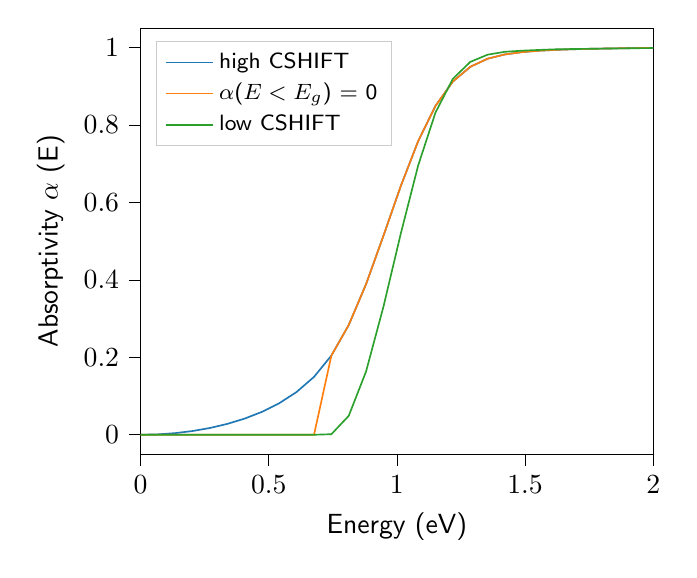
\begin{tikzpicture}

\definecolor{color0}{rgb}{0.12156862745098,0.466666666666667,0.705882352941177}
\definecolor{color1}{rgb}{1,0.498039215686275,0.0549019607843137}
\definecolor{color2}{rgb}{0.172549019607843,0.627450980392157,0.172549019607843}

\begin{axis}[
legend cell align={left},
legend style={fill opacity=0.8, draw opacity=1, text opacity=1, at={(0.03,0.97)}, anchor=north west, draw=white!80.0!black},
tick align=outside,
tick pos=left,
x grid style={white!69.01960784313725!black},
xlabel={Energy (eV)},
xmin=0, xmax=2,
xtick style={color=black},
y grid style={white!69.01960784313725!black},
ylabel={Absorptivity \(\displaystyle \alpha\) (E)},
ymin=-0.05, ymax=1.05,
ytick style={color=black}
]
\addplot [semithick, color0]
table {%
0 0
0.0677 0.00105069948951619
0.1354 0.00423565010418236
0.2031 0.00966440604560037
0.2708 0.0174889910212335
0.3385 0.0280596473197948
0.4062 0.0417245295140892
0.4739 0.0592161616746564
0.5415 0.0815656890385469
0.6092 0.11063318149478
0.6769 0.149570425633838
0.7446 0.204538179679961
0.8123 0.283567384906138
0.88 0.389212439270968
0.9477 0.513934494137355
1.0154 0.642448080658341
1.0831 0.75828048268401
1.1508 0.84954137563106
1.2185 0.91224899756501
1.2862 0.95023539714835
1.3539 0.971216790890076
1.4216 0.982343877481651
1.4892 0.988386186782393
1.5569 0.991980776043341
1.6246 0.994286461452083
1.6923 0.995801502686318
1.76 0.996887597878625
1.8277 0.997723722542282
1.8954 0.99837665977387
1.9631 0.998886352796302
2.0308 0.999277492452979
2.0985 0.999565386125146
2.1662 0.99975821913913
2.2339 0.999873138262864
2.3016 0.999938834082579
2.3693 0.999972823175914
2.437 0.99998873930106
2.5046 0.99999575639937
2.5723 0.999998730116318
2.64 0.999999703286655
2.7077 0.999999940613374
2.7754 0.999999988142873
2.8431 0.999999997106652
2.9108 0.999999998982937
2.9785 0.99999999943325
3.0462 0.999999999566765
3.1139 0.999999999633227
3.1816 0.999999999702733
3.2493 0.99999999978093
3.317 0.999999999854024
3.3847 0.999999999907744
3.4523 0.999999999941054
3.52 0.999999999961334
3.5877 0.999999999972889
3.6554 0.99999999997815
3.7231 0.999999999981021
3.7908 0.999999999986044
3.8585 0.999999999992035
3.9262 0.999999999996533
3.9939 0.999999999998808
4.0616 0.999999999999643
4.1293 0.999999999999911
4.197 0.999999999999984
4.2647 0.999999999999998
4.3324 1
4.4001 1
4.4677 1
4.5354 1
4.6031 1
4.6708 1
4.7385 1
4.8062 1
4.8739 1
4.9416 1
5.0093 1
5.077 1
5.1447 1
5.2124 1
5.2801 1
5.3478 1
5.4154 1
5.4831 1
5.5508 1
5.6185 1
5.6862 1
5.7539 1
5.8216 1
5.8893 1
5.957 1
6.0247 1
6.0924 1
6.1601 1
6.2278 1
6.2955 1
6.3632 1
6.4308 1
6.4985 1
6.5662 1
6.6339 1
6.7016 1
6.7693 1
6.837 1
6.9047 1
6.9724 1
7.0401 1
7.1078 1
7.1755 1
7.2432 1
7.3109 1
7.3785 1
7.4462 1
7.5139 1
7.5816 1
7.6493 1
7.717 1
7.7847 1
7.8524 1
7.9201 1
7.9878 1
8.0555 1
8.1232 1
8.1909 1
8.2586 1
8.3262 1
8.3939 1
8.4616 1
8.5293 1
8.597 1
8.6647 1
8.7324 1
8.8001 1
8.8678 1
8.9355 1
9.0032 1
9.0709 1
9.1386 1
9.2063 1
9.274 1
9.3416 1
9.4093 1
9.477 1
9.5447 1
9.6124 1
9.6801 1
9.7478 1
9.8155 1
9.8832 1
9.9509 1
10.0186 1
10.0863 1
10.154 1
10.2217 1
10.2893 1
10.357 1
10.4247 1
10.4924 1
10.5601 1
10.6278 1
10.6955 1
10.7632 1
10.8309 1
10.8986 1
10.9663 1
11.034 1
11.1017 1
11.1694 1
11.2371 1
11.3047 1
11.3724 1
11.4401 1
11.5078 1
11.5755 1
11.6432 1
11.7109 1
11.7786 1
11.8463 1
11.914 1
11.9817 1
12.0494 1
12.1171 1
12.1848 1
12.2524 1
12.3201 1
12.3878 1
12.4555 1
12.5232 1
12.5909 1
12.6586 1
12.7263 1
12.794 1
12.8617 1
12.9294 1
12.9971 1
13.0648 1
13.1325 1
13.2002 1
13.2678 1
13.3355 1
13.4032 1
13.4709 1
13.5386 1
13.6063 1
13.674 1
13.7417 1
13.8094 1
13.8771 1
13.9448 1
14.0125 1
14.0802 1
14.1479 1
14.2155 1
14.2832 1
14.3509 1
14.4186 1
14.4863 1
14.554 1
14.6217 1
14.6894 1
14.7571 1
14.8248 1
14.8925 1
14.9602 1
15.0279 1
15.0956 1
15.1633 1
15.2309 1
15.2986 1
15.3663 1
15.434 1
15.5017 1
15.5694 1
15.6371 1
15.7048 1
15.7725 1
15.8402 1
15.9079 1
15.9756 1
16.0433 1
16.111 1
16.1786 1
16.2463 1
16.314 1
16.3817 1
16.4494 1
16.5171 1
16.5848 1
16.6525 1
16.7202 1
16.7879 1
16.8556 1
16.9233 1
16.991 1
17.0587 1
17.1264 1
17.194 1
17.2617 1
17.3294 1
17.3971 1
17.4648 1
17.5325 1
17.6002 1
17.6679 1
17.7356 1
17.8033 1
17.871 1
17.9387 1
18.0064 1
18.0741 1
18.1417 1
18.2094 1
18.2771 1
18.3448 1
18.4125 1
18.4802 1
18.5479 1
18.6156 1
18.6833 1
18.751 1
18.8187 1
18.8864 1
18.9541 1
19.0218 1
19.0895 1
19.1571 1
19.2248 1
19.2925 1
19.3602 1
19.4279 1
19.4956 1
19.5633 1
19.631 1
19.6987 1
19.7664 1
19.8341 1
19.9018 1
19.9695 1
20.0372 1
20.1048 1
20.1725 1
20.2402 1
20.3079 1
20.3756 1
20.4433 1
20.511 1
20.5787 1
20.6464 1
20.7141 1
20.7818 1
20.8495 1
20.9172 1
20.9849 1
21.0525 1
21.1202 1
21.1879 1
21.2556 1
21.3233 1
21.391 1
21.4587 1
21.5264 1
21.5941 1
21.6618 1
21.7295 1
21.7972 1
21.8649 1
21.9326 1
22.0003 1
22.0679 1
22.1356 1
22.2033 1
22.271 1
22.3387 1
22.4064 1
22.4741 1
22.5418 1
22.6095 1
22.6772 1
22.7449 1
22.8126 1
22.8803 1
22.948 1
23.0156 1
23.0833 1
23.151 1
23.2187 1
23.2864 1
23.3541 1
23.4218 1
23.4895 1
23.5572 1
23.6249 1
23.6926 1
23.7603 1
23.828 1
23.8957 1
23.9634 1
24.031 1
24.0987 1
24.1664 1
24.2341 1
24.3018 1
24.3695 1
24.4372 1
24.5049 1
24.5726 1
24.6403 1
24.708 1
24.7757 1
24.8434 1
24.9111 1
24.9787 1
25.0464 1
25.1141 1
25.1818 1
25.2495 1
25.3172 1
25.3849 1
25.4526 1
25.5203 1
25.588 1
25.6557 1
25.7234 1
25.7911 1
25.8588 0.999999999999999
25.9265 0.999999999999999
25.9941 0.999999999999998
26.0618 0.999999999999998
26.1295 0.999999999999998
26.1972 0.999999999999998
26.2649 0.999999999999999
26.3326 0.999999999999999
26.4003 0.999999999999999
26.468 0.999999999999999
26.5357 0.999999999999999
26.6034 0.999999999999999
26.6711 0.999999999999999
26.7388 0.999999999999999
26.8065 1
26.8742 1
26.9418 1
27.0095 1
27.0772 1
27.1449 1
27.2126 0.999999999999999
27.2803 0.999999999999999
27.348 0.999999999999998
27.4157 0.999999999999997
27.4834 0.999999999999997
27.5511 0.999999999999996
27.6188 0.999999999999996
27.6865 0.999999999999996
27.7542 0.999999999999996
27.8219 0.999999999999995
27.8896 0.999999999999994
27.9572 0.999999999999992
28.0249 0.99999999999999
28.0926 0.999999999999985
28.1603 0.999999999999979
28.228 0.999999999999973
28.2957 0.999999999999969
28.3634 0.999999999999967
28.4311 0.999999999999965
28.4988 0.999999999999959
28.5665 0.999999999999946
28.6342 0.999999999999929
28.7019 0.999999999999908
28.7696 0.999999999999893
28.8373 0.999999999999899
28.9049 0.999999999999923
28.9726 0.999999999999949
29.0403 0.999999999999964
29.108 0.999999999999971
29.1757 0.999999999999973
29.2434 0.999999999999975
29.3111 0.99999999999998
29.3788 0.999999999999987
29.4465 0.999999999999992
29.5142 0.999999999999996
29.5819 0.999999999999998
29.6496 0.999999999999999
29.7173 0.999999999999999
29.785 0.999999999999999
29.8527 0.999999999999999
29.9203 1
29.988 1
30.0557 0.999999999999999
30.1234 0.999999999999999
30.1911 0.999999999999999
30.2588 0.999999999999999
30.3265 0.999999999999997
30.3942 0.999999999999994
30.4619 0.999999999999993
30.5296 0.999999999999996
30.5973 0.999999999999998
30.665 0.999999999999999
30.7327 1
30.8004 1
30.868 1
30.9357 1
31.0034 1
31.0711 1
31.1388 1
31.2065 1
31.2742 1
31.3419 0.999999999999999
31.4096 0.999999999999999
31.4773 0.999999999999998
31.545 0.999999999999998
31.6127 0.999999999999998
31.6804 0.999999999999998
31.7481 0.999999999999998
31.8158 0.999999999999997
31.8834 0.999999999999996
31.9511 0.999999999999994
32.0188 0.999999999999993
32.0865 0.999999999999991
32.1542 0.999999999999988
32.2219 0.999999999999986
32.2896 0.999999999999986
32.3573 0.999999999999989
32.425 0.999999999999992
32.4927 0.999999999999995
32.5604 0.999999999999996
32.6281 0.999999999999996
32.6958 0.999999999999996
32.7635 0.999999999999995
32.8311 0.999999999999993
32.8988 0.99999999999999
32.9665 0.999999999999985
33.0342 0.999999999999981
33.1019 0.999999999999981
33.1696 0.999999999999982
33.2373 0.99999999999998
33.305 0.999999999999972
33.3727 0.999999999999951
33.4404 0.999999999999915
33.5081 0.99999999999988
33.5758 0.999999999999856
33.6435 0.999999999999844
33.7112 0.999999999999854
33.7788 0.999999999999884
33.8465 0.999999999999913
33.9142 0.999999999999931
33.9819 0.999999999999945
34.0496 0.999999999999959
34.1173 0.999999999999971
34.185 0.999999999999981
34.2527 0.999999999999983
34.3204 0.999999999999979
34.3881 0.999999999999972
34.4558 0.999999999999964
34.5235 0.999999999999957
34.5912 0.99999999999995
34.6589 0.999999999999945
34.7266 0.999999999999942
34.7942 0.999999999999939
34.8619 0.999999999999937
34.9296 0.999999999999941
34.9973 0.999999999999948
35.065 0.999999999999954
35.1327 0.999999999999956
35.2004 0.999999999999955
35.2681 0.99999999999995
35.3358 0.999999999999942
35.4035 0.999999999999931
35.4712 0.999999999999914
35.5389 0.999999999999896
35.6066 0.999999999999879
35.6743 0.999999999999853
35.7419 0.999999999999792
35.8096 0.999999999999693
35.8773 0.999999999999589
35.945 0.999999999999528
36.0127 0.999999999999496
36.0804 0.999999999999432
36.1481 0.999999999999286
36.2158 0.999999999999048
36.2835 0.999999999998785
36.3512 0.99999999999865
36.4189 0.999999999998609
36.4866 0.999999999998589
36.5543 0.999999999998647
36.622 0.999999999998806
36.6897 0.99999999999894
36.7573 0.999999999999052
36.825 0.9999999999991
36.8927 0.999999999999086
36.9604 0.999999999998931
37.0281 0.999999999998538
37.0958 0.999999999998077
37.1635 0.99999999999774
37.2312 0.999999999997593
37.2989 0.999999999997704
37.3666 0.999999999998157
37.4343 0.999999999998732
37.502 0.999999999999182
37.5697 0.999999999999463
37.6374 0.999999999999632
37.705 0.999999999999738
37.7727 0.999999999999804
37.8404 0.999999999999856
37.9081 0.999999999999893
37.9758 0.999999999999907
38.0435 0.999999999999903
38.1112 0.999999999999877
38.1789 0.999999999999849
38.2466 0.999999999999835
38.3143 0.999999999999813
38.382 0.999999999999784
38.4497 0.999999999999748
38.5174 0.999999999999722
38.5851 0.999999999999701
38.6528 0.99999999999971
38.7204 0.999999999999727
38.7881 0.999999999999739
38.8558 0.999999999999732
38.9235 0.999999999999714
38.9912 0.999999999999682
39.0589 0.999999999999624
39.1266 0.999999999999547
39.1943 0.999999999999433
39.262 0.999999999999339
39.3297 0.999999999999328
39.3974 0.999999999999378
39.4651 0.999999999999413
39.5328 0.999999999999419
39.6005 0.999999999999441
39.6681 0.99999999999948
39.7358 0.999999999999537
39.8035 0.999999999999561
39.8712 0.999999999999545
39.9389 0.999999999999488
40.0066 0.999999999999433
40.0743 0.999999999999395
40.142 0.999999999999339
40.2097 0.999999999999311
40.2774 0.999999999999369
40.3451 0.999999999999478
40.4128 0.99999999999956
40.4805 0.999999999999606
40.5482 0.999999999999608
40.6159 0.999999999999568
40.6835 0.999999999999485
40.7512 0.9999999999993
40.8189 0.99999999999896
40.8866 0.999999999998559
40.9543 0.999999999998311
41.022 0.999999999998277
41.0897 0.999999999998274
41.1574 0.999999999998226
41.2251 0.999999999998081
41.2928 0.999999999997728
41.3605 0.999999999996881
41.4282 0.999999999994736
41.4959 0.999999999990059
41.5636 0.999999999981031
41.6312 0.999999999967993
41.6989 0.999999999956588
41.7666 0.999999999950057
41.8343 0.999999999943391
41.902 0.999999999934755
41.9697 0.999999999928763
42.0374 0.999999999930093
42.1051 0.999999999929125
42.1728 0.999999999923494
42.2405 0.999999999915809
42.3082 0.999999999908758
42.3759 0.999999999898159
42.4436 0.999999999880087
42.5113 0.999999999866869
42.579 0.999999999868002
42.6466 0.999999999872548
42.7143 0.999999999879831
42.782 0.999999999899063
42.8497 0.999999999919186
42.9174 0.999999999935674
42.9851 0.999999999949564
43.0528 0.999999999956182
43.1205 0.999999999952705
43.1882 0.999999999937436
43.2559 0.999999999911856
43.3236 0.999999999889946
43.3913 0.999999999888469
43.459 0.999999999880608
43.5267 0.999999999851882
43.5943 0.999999999794311
43.662 0.999999999690437
43.7297 0.999999999526063
43.7974 0.999999999291474
43.8651 0.999999999081299
43.9328 0.999999999023171
44.0005 0.99999999908014
44.0682 0.999999999138306
44.1359 0.99999999919633
44.2036 0.999999999207392
44.2713 0.999999999198545
44.339 0.99999999909659
44.4067 0.999999998911449
44.4744 0.99999999889792
44.5421 0.99999999909933
44.6097 0.999999999255829
44.6774 0.999999999426738
44.7451 0.999999999549359
44.8128 0.999999999619591
44.8805 0.999999999669943
44.9482 0.999999999713317
45.0159 0.999999999763374
45.0836 0.999999999803022
45.1513 0.99999999984795
45.219 0.999999999894294
45.2867 0.999999999931328
45.3544 0.999999999955181
45.4221 0.999999999965714
45.4898 0.999999999966295
45.5574 0.999999999959675
45.6251 0.999999999948662
45.6928 0.999999999936738
45.7605 0.99999999993166
45.8282 0.999999999934544
45.8959 0.999999999938578
45.9636 0.99999999994481
46.0313 0.999999999951238
46.099 0.999999999959942
46.1667 0.999999999967517
46.2344 0.999999999974409
46.3021 0.999999999980325
46.3698 0.99999999998433
46.4375 0.999999999985894
46.5051 0.999999999985223
46.5728 0.999999999980697
46.6405 0.999999999969444
46.7082 0.999999999946873
46.7759 0.999999999915836
46.8436 0.999999999876397
46.9113 0.999999999821365
46.979 0.999999999747502
47.0467 0.999999999653932
47.1144 0.999999999561791
47.1821 0.999999999444838
47.2498 0.999999999301304
47.3175 0.999999999140377
47.3852 0.999999999038147
47.4529 0.999999998987859
47.5205 0.999999999059056
47.5882 0.999999999223505
47.6559 0.999999999395695
47.7236 0.999999999540578
47.7913 0.999999999646847
47.859 0.999999999709718
47.9267 0.999999999740432
47.9944 0.999999999746151
48.0621 0.999999999735197
48.1298 0.999999999716417
48.1975 0.999999999684935
48.2652 0.999999999617128
48.3329 0.99999999947096
48.4006 0.999999999170809
48.4682 0.999999998766572
48.5359 0.9999999983904
48.6036 0.999999998134359
48.6713 0.999999997919971
48.739 0.999999997658275
48.8067 0.999999997481093
48.8744 0.999999997315625
48.9421 0.999999997004392
49.0098 0.999999996800098
49.0775 0.999999996786402
49.1452 0.999999996926187
49.2129 0.999999997094792
49.2806 0.999999996991437
49.3483 0.999999996810168
49.416 0.999999997016331
49.4836 0.999999997455555
49.5513 0.999999997971129
49.619 0.999999998512727
49.6867 0.99999999894423
49.7544 0.999999999300348
49.8221 0.999999999526438
49.8898 0.999999999675118
49.9575 0.999999999770523
50.0252 0.999999999816703
50.0929 0.999999999810149
50.1606 0.99999999978259
50.2283 0.999999999746301
50.296 0.999999999736322
50.3637 0.999999999772775
50.4313 0.999999999814263
50.499 0.999999999850627
50.5667 0.999999999870836
50.6344 0.999999999890015
50.7021 0.999999999891729
50.7698 0.99999999987078
50.8375 0.999999999846532
50.9052 0.999999999810707
50.9729 0.999999999742881
51.0406 0.999999999614486
51.1083 0.999999999376162
51.176 0.999999999072136
51.2437 0.999999998403454
51.3114 0.999999997023737
51.3791 0.99999999542198
51.4467 0.999999994255105
51.5144 0.999999992589191
51.5821 0.999999991120275
51.6498 0.999999990425391
51.7175 0.999999990912368
51.7852 0.999999991744384
51.8529 0.999999992307524
51.9206 0.999999991738309
51.9883 0.999999990460643
52.056 0.999999989676014
52.1237 0.999999989946355
52.1914 0.999999991057621
52.2591 0.999999992168818
52.3268 0.999999992162281
52.3944 0.999999991582597
52.4621 0.999999990876181
52.5298 0.999999989809655
52.5975 0.999999987899418
52.6652 0.999999986280398
52.7329 0.999999984444934
52.8006 0.999999982007974
52.8683 0.999999979947209
52.936 0.99999997891742
53.0037 0.999999978071913
53.0714 0.999999977245948
53.1391 0.999999974191647
53.2068 0.999999970623969
53.2745 0.999999968143993
53.3422 0.999999965030938
53.4098 0.999999965190761
53.4775 0.999999968632414
53.5452 0.999999973446418
53.6129 0.999999978685618
53.6806 0.999999982078224
53.7483 0.999999984791602
53.816 0.999999987241259
53.8837 0.999999990038645
53.9514 0.999999992722216
54.0191 0.99999999395034
54.0868 0.999999992942321
54.1545 0.999999988847991
54.2222 0.999999984643218
54.2899 0.999999983218566
54.3575 0.999999982498213
54.4252 0.999999979403688
54.4929 0.999999974651196
54.5606 0.999999972608912
54.6283 0.999999972768461
54.696 0.999999973323946
54.7637 0.999999971471389
54.8314 0.999999965535079
54.8991 0.999999953279126
54.9668 0.999999930836998
55.0345 0.999999905359219
55.1022 0.999999874471674
55.1699 0.999999840187219
55.2376 0.99999978620542
55.3053 0.999999682809144
55.3729 0.999999480928828
55.4406 0.999999174908307
55.5083 0.999998687599918
55.576 0.999997610263565
55.6437 0.999994727713738
55.7114 0.999985999052962
55.7791 0.999961322728108
55.8468 0.999897088990551
55.9145 0.99970108521071
55.9822 0.99908974156979
56.0499 0.997304509279095
56.1176 0.992876513382954
56.1853 0.98357533755363
56.253 0.967682912385169
56.3206 0.942795014288814
56.3883 0.907950365060206
56.456 0.863910057568136
56.5237 0.81514256002743
56.5914 0.761829593149554
56.6591 0.708939400694187
56.7268 0.655439636169112
56.7945 0.617127415139221
56.8622 0.579044406149439
56.9299 0.546856135965056
56.9976 0.517312881657507
57.0653 0.485863158533444
57.133 0.46943140786056
57.2007 0.452482241935271
57.2684 0.434983489920214
57.336 0.416915402963832
57.4037 0.417067931546838
57.4714 0.398425430601574
57.5391 0.398597627960086
57.6068 0.379338360904361
57.6745 0.379510585847089
57.7422 0.359617215575955
57.8099 0.35979412640148
57.8776 0.339247128211901
57.9453 0.339421805336417
58.013 0.339601710169316
58.0807 0.318360699663916
58.1484 0.318531846659272
58.2161 0.318713084913718
58.2837 0.318893713673575
58.3514 0.296914919200874
58.4191 0.297095686704716
58.4868 0.297271460429315
58.5545 0.297451918130871
58.6222 0.297627386604688
58.6899 0.274876511497583
58.7576 0.275050022216943
58.8253 0.275223388670184
58.893 0.275410208212769
58.9607 0.275583282626076
59.0284 0.275765273758567
59.0961 0.252182370131557
59.1638 0.252355474454346
59.2314 0.252523868445243
59.2991 0.252688289472262
59.3668 0.252860993593704
59.4345 0.253033564102081
59.5022 0.25320600120425
59.5699 0.253390922347277
59.6376 0.22891016247583
59.7053 0.229068136348254
59.773 0.229233714596424
59.8407 0.229395313288755
59.9084 0.229556793967197
59.9761 0.229722017466935
60.0438 0.229890983871685
60.1115 0.230048250240787
60.1792 0.230216981047127
60.2468 0.230385260035068
60.3145 0.2305537565638
60.3822 0.20508108921344
60.4499 0.205233228529534
60.5176 0.205385266507788
60.5853 0.205537203281889
60.653 0.205689038985262
60.7207 0.205840773751072
60.7884 0.205995900320147
60.8561 0.206154420052154
60.9238 0.206305853468451
60.9915 0.206460680297928
61.0592 0.206618901877267
61.1269 0.206773529903664
61.1945 0.206931253438909
61.2622 0.20708568328805
61.3299 0.198427753924296
61.3976 0.180643904187932
61.4653 0.180780481488953
61.533 0.180920074780319
61.6007 0.181062685930799
61.6684 0.181199013518025
61.7361 0.181341460832133
61.8038 0.181480724691235
61.8715 0.181623009285277
61.9392 0.181765213025812
62.0069 0.181907336000799
62.0746 0.182049378298052
62.1423 0.182191340005249
62.2099 0.1823329566276
62.2776 0.182474757522937
62.3453 0.182616478090323
62.413 0.182758118416877
62.4807 0.182899678589581
62.5484 0.183044269167491
62.6161 0.183185670011033
62.6838 0.183333215262376
62.7515 0.1834744578272
62.8192 0.155543031990747
62.8869 0.155664646942187
62.9546 0.155791568171079
63.0223 0.155915740979059
63.09 0.15603716294757
63.1576 0.156163669482446
63.2253 0.156287652245297
63.293 0.156414261762263
63.3607 0.156538118904508
63.4284 0.156664604698381
63.4961 0.156788336461285
63.5638 0.156914698764941
63.6315 0.157038305389096
63.6992 0.157164544434769
63.7669 0.157288026160095
63.8346 0.157416839377114
63.9023 0.157542895385339
63.97 0.157666191409458
64.0377 0.157794824754226
64.1054 0.157920698225996
64.173 0.158043583365983
64.2407 0.158172037392509
64.3084 0.158300432803087
64.3761 0.158426064674213
64.4438 0.15854893027185
64.5115 0.15867714692509
64.5792 0.158805305165016
64.6469 0.158933405040641
64.7146 0.159061446600921
64.7823 0.159186718957612
64.85 0.159314642975416
64.9177 0.159437083149775
64.9854 0.159564888773567
65.0531 0.129937332135193
65.1207 0.130042916459491
65.1884 0.13014864214083
65.2561 0.130254323053701
65.3238 0.130359959234426
65.3915 0.130465550719283
65.4592 0.130571097544508
65.5269 0.130676599746293
65.5946 0.130782057360788
65.6623 0.130891984933443
65.73 0.130999613688983
65.7977 0.131104940526802
65.8654 0.131210222916833
65.9331 0.131315460895018
66.0008 0.131420654497259
66.0685 0.131525803759415
66.1361 0.131635251500305
66.2038 0.131742579212096
66.2715 0.131847598458127
66.3392 0.131952573502432
66.4069 0.132057504380668
66.4746 0.13216919818916
66.5423 0.132274043559848
66.61 0.132378844866586
66.6777 0.132483602144869
66.7454 0.132595134411324
66.8131 0.132699806438497
66.8808 0.132804434538881
66.9485 0.132915846890919
67.0162 0.133020389929515
67.0838 0.13312470453487
67.1515 0.133235997266317
67.2192 0.133340411659157
67.2869 0.133451626001041
67.3546 0.133555955643219
67.4223 0.133660241626562
67.49 0.133771336713874
67.5577 0.133875538134278
67.6254 0.133986555097483
67.6931 0.134090672076778
67.7608 0.134197033928768
67.8285 0.134305643679722
67.8962 0.134411923390049
67.9639 0.134520453168319
68.0316 0.134626650852338
68.0992 0.134734916887635
68.1669 0.134841032709957
68.2346 0.134949402917436
68.3023 0.135055436943412
68.37 0.135163727505718
68.4377 0.135274277946555
68.5054 0.135377890875895
68.5731 0.135488363916906
68.6408 0.135594195422619
68.7085 0.135702288994792
68.7762 0.135808039100122
68.8439 0.135916053402536
68.9116 0.136026335214065
68.9793 0.136131964890917
69.0469 0.136239678910069
69.1146 0.125730833150118
69.1823 0.104192968515315
69.25 0.104278622874911
69.3177 0.104360652102977
69.3854 0.104444452447481
69.4531 0.104530026624944
69.5208 0.104611970324499
69.5885 0.104695687891634
69.6562 0.104781182033388
69.7239 0.104863040369582
69.7916 0.104946675314921
69.8593 0.105032089566997
69.927 0.105113862704521
69.9947 0.105199223777745
70.0623 0.105282607624899
70.13 0.105367916596224
70.1977 0.105449577216698
70.2654 0.105533020897955
70.3331 0.10561825031573
70.4008 0.105699826116836
70.4685 0.105785002579345
70.5362 0.105868337697638
70.6039 0.105953462245331
70.6716 0.106034925992541
70.7393 0.106119997711264
70.807 0.106203224531485
70.8747 0.106288244457461
70.9424 0.106369596431479
71.01 0.106454422018463
71.0777 0.106537540835703
71.1454 0.106622456416309
71.2131 0.106703696930214
71.2808 0.106788559933099
71.3485 0.106871570979196
71.4162 0.106956382432184
71.4839 0.107037511731236
71.5516 0.107122270731487
71.6193 0.107205174268544
71.687 0.107286219761776
71.7547 0.107370900201614
71.8224 0.107453722631236
71.8901 0.107538351733789
71.9577 0.107619145294694
72.0254 0.107703722192345
72.0931 0.107786437603316
72.1608 0.107870963283735
72.2285 0.107951787633178
72.2962 0.108034422285469
72.3639 0.108118869824692
72.4316 0.119474694300775
72.4993 0.119565260844019
72.567 0.141813231065151
72.6347 0.141914374222057
72.7024 0.14202257440614
72.7701 0.142126004530285
72.8378 0.14223176325657
72.9055 0.142332746245761
72.9731 0.142440617243622
73.0408 0.142541520368611
73.1085 0.142649497834538
73.1762 0.142750321157297
73.2439 0.142855850745467
73.3116 0.1539038481286
73.3793 0.154011547869303
73.447 0.164940225961518
73.5147 0.186302198636223
73.5824 0.196853345141814
73.6501 0.20728314730877
73.7178 0.23754316431558
73.7855 0.247488628722033
73.8532 0.276284560116559
73.9208 0.285766143201499
73.9885 0.313164298962682
74.0562 0.348056623412625
74.1239 0.381224631586205
74.1916 0.412739804680086
74.2593 0.442702867934937
74.327 0.491414780682331
74.3947 0.523691704412821
74.4624 0.553970039008268
74.5301 0.593116385165064
74.5978 0.633688870358703
74.6655 0.665963510160352
74.7332 0.683255043704582
74.8009 0.703578197634912
74.8686 0.711521574496317
74.9362 0.726502283558152
75.0039 0.737299529444236
75.0716 0.757401344975029
75.1393 0.787444861936698
75.207 0.818639058018789
75.2747 0.855139647063684
75.3424 0.888829993398358
75.4101 0.91804701261229
75.4778 0.938035140200342
75.5455 0.947292095737844
75.6132 0.94953247077932
75.6809 0.944115907565916
75.7486 0.926463533412649
75.8163 0.884842646914669
75.8839 0.839745040751555
75.9516 0.809717368578319
76.0193 0.802141257083471
76.087 0.812517053132977
76.1547 0.831587380748456
76.2224 0.85272143589644
76.2901 0.876264513741737
76.3578 0.89744900069717
76.4255 0.917265196425476
76.4932 0.938411088136105
76.5609 0.954171321069411
76.6286 0.968968258201481
76.6963 0.980366926832262
76.764 0.987602652539513
76.8317 0.991067736700046
76.8993 0.992748346791415
76.967 0.992806955754858
77.0347 0.990527582956696
77.1024 0.985301057213127
77.1701 0.978630466072733
77.2378 0.973186727748449
77.3055 0.969791984107192
77.3732 0.970270314099373
77.4409 0.973035218802058
77.5086 0.974207393193243
77.5763 0.972137396523732
77.644 0.959947211828125
77.7117 0.943868036685591
77.7794 0.930331825654047
77.847 0.924498294783209
77.9147 0.926615471626339
77.9824 0.931535313424046
78.0501 0.937842770877118
78.1178 0.950758817643922
78.1855 0.9664379730996
78.2532 0.97895099910076
78.3209 0.986819564906969
78.3886 0.991061446969259
78.4563 0.992772651361842
78.524 0.991989365481872
78.5917 0.989937906004885
78.6594 0.988500658103197
78.7271 0.9890041906526
78.7948 0.990460560227821
78.8624 0.992067391144912
78.9301 0.992226663712449
78.9978 0.990885940038322
79.0655 0.98771310866668
79.1332 0.981729581895407
79.2009 0.971239136026701
79.2686 0.956507393795032
79.3363 0.935068432564262
79.404 0.911963274852495
79.4717 0.89891869129991
79.5394 0.900381630611813
79.6071 0.918062926424025
79.6748 0.93974161429126
79.7425 0.958699979667985
79.8101 0.970114358328946
79.8778 0.97684108014552
79.9455 0.979096776540121
80.0132 0.976407407760143
80.0809 0.971414693830652
80.1486 0.966765081284506
80.2163 0.960248551156081
80.284 0.946774884219753
80.3517 0.929668588648785
80.4194 0.91449185491491
80.4871 0.909657167151888
80.5548 0.914721736591272
80.6225 0.927084245870918
80.6902 0.93408064517
80.7579 0.93697377192815
80.8255 0.932540826957259
80.8932 0.92464255686761
80.9609 0.916963380663634
81.0286 0.908488098572146
81.0963 0.904683185916236
81.164 0.903488189846865
81.2317 0.907672781033348
81.2994 0.910430853435007
81.3671 0.909347353364231
81.4348 0.902874998060501
81.5025 0.892914379731073
81.5702 0.874998974782576
81.6379 0.847632990442718
81.7056 0.824490308303105
81.7732 0.800642736580134
81.8409 0.789115434227397
81.9086 0.795252069947095
81.9763 0.804050114212816
82.044 0.81777545452667
82.1117 0.832985236586234
82.1794 0.844756607822916
82.2471 0.851521876589589
82.3148 0.849626952483528
82.3825 0.838675395826459
82.4502 0.826900847729255
82.5179 0.816888255620994
82.5856 0.803459111888512
82.6533 0.800832479234296
82.721 0.79814946001404
82.7886 0.806907640458824
82.8563 0.820575236890572
82.924 0.833314508613179
82.9917 0.833558144338447
83.0594 0.828920581013461
83.1271 0.818965844088435
83.1948 0.808414549172201
83.2625 0.794244048045844
83.3302 0.791451380799343
83.3979 0.791658912637572
83.4656 0.806459459355078
83.5333 0.830422143987838
83.601 0.849295211440028
83.6687 0.85172739648685
83.7363 0.84535115754439
83.804 0.831463571736463
83.8717 0.816279692969027
83.9394 0.799677919392485
84.0071 0.79395754314384
84.0748 0.794167839194229
84.1425 0.800330446427268
84.2102 0.817355838392924
84.2779 0.828004764645449
84.3456 0.830772119113932
84.4133 0.82598966694712
84.481 0.810198502845548
84.5487 0.795970661213571
84.6164 0.780627426908458
84.684 0.76409916176044
84.7517 0.76432921757038
84.8194 0.757506113604117
84.8871 0.768242575966182
84.9548 0.775225647470447
85.0225 0.785219297011948
85.0902 0.788633994857073
85.1579 0.791987758671384
85.2256 0.789138670521513
85.2933 0.78939343528819
85.361 0.786495595457442
85.4287 0.780301184878571
85.4964 0.780547243995159
85.5641 0.790363044221457
85.6318 0.79372263937265
85.6994 0.790891882619502
85.7671 0.781592647112356
85.8348 0.771851836938619
85.9025 0.761654454261235
85.9702 0.747234411511074
86.0379 0.735898960778475
86.1056 0.719874498773472
86.1733 0.707251188886347
86.241 0.694033893774231
86.3087 0.68496862474466
86.3764 0.685189740118367
86.4441 0.70374738870527
86.5118 0.745285091406997
86.5795 0.787580607091169
86.6471 0.80908828439186
86.7148 0.815027483521843
86.7825 0.803814126116061
86.8502 0.79500517593947
86.9179 0.782518312792776
86.9856 0.762152721267165
87.0533 0.74759714401518
87.121 0.736132221032835
87.1887 0.711300000514319
87.2564 0.698130268558576
87.3241 0.679520130636638
87.3918 0.654520504976625
87.4595 0.638666136421701
87.5272 0.633380116320514
87.5949 0.622326010290099
87.6625 0.633890006011028
87.7302 0.634154557274939
87.7979 0.628821807356975
87.8656 0.611706403890226
87.9333 0.59378216391855
88.001 0.581427840777096
88.0687 0.575224608566564
88.1364 0.575478482764676
88.2041 0.575719368675967
88.2718 0.575979273218019
88.3395 0.582680072869835
88.4072 0.582927389007569
88.4749 0.595791445980918
88.5426 0.596071516604861
88.6102 0.596331659500497
88.6779 0.583997761366616
88.7456 0.577805808284074
88.8133 0.564852249895333
88.881 0.565109063113808
88.9487 0.544766503102204
89.0164 0.545007599890641
89.0841 0.552227234739816
89.1518 0.552481595641385
89.2195 0.538678196925904
89.2872 0.538917587062654
89.3549 0.517236516666757
89.4226 0.517465757876169
89.4903 0.502494875947635
89.558 0.525337575566944
89.6256 0.54716956171054
89.6933 0.568030239872866
89.761 0.606754461064891
89.8287 0.636445055863154
89.8964 0.653302822686172
89.9641 0.669401625335155
90.0318 0.684780926238908
90.0995 0.699465940324331
90.1672 0.704404960525403
90.2349 0.713774603548447
90.3026 0.704964404189724
90.3703 0.691054640751351
90.438 0.681491105191003
90.5057 0.67161005223209
90.5733 0.661406892499521
90.641 0.656305712433118
90.7087 0.656566893018505
90.7764 0.656821421888471
90.8441 0.651642234200154
90.9118 0.640756735774382
90.9795 0.63530833330378
91.0472 0.641278283309351
91.1149 0.641532300927294
91.1826 0.641786113004757
91.2503 0.642046163568744
91.318 0.653450323805535
91.3857 0.653709613325761
91.4534 0.642844404340156
91.5211 0.643116513059719
91.5887 0.643368686234117
91.6564 0.626246295222647
91.7241 0.620537667441945
91.7918 0.608540004981231
91.8595 0.608791398356697
91.9272 0.60276959264831
91.9949 0.603026741026143
92.0626 0.603277283222025
92.1303 0.597165698745186
92.198 0.577667976650419
92.2657 0.577916078603216
92.3334 0.564460861576189
92.4011 0.564688190705614
92.4688 0.578640242863233
92.5364 0.578887269181628
92.6041 0.598897417006621
92.6718 0.599165207740329
92.7395 0.60581076233171
92.8072 0.593212275339804
92.8749 0.586892061061181
92.9426 0.573654539837231
93.0103 0.552819931708272
93.078 0.545805937766779
93.1457 0.531176124893614
93.2134 0.516047871069864
93.2811 0.516284477030045
93.3488 0.516520943477649
93.4165 0.516757270509732
93.4842 0.516993458223274
93.5518 0.524978699439789
93.6195 0.517471185090481
93.6872 0.517719246974777
93.7549 0.517954879994242
93.8226 0.502297425090789
93.8903 0.502517606148539
93.958 0.518648651786127
94.0257 0.518902172724929
94.0934 0.519137112948332
94.1611 0.519371914807588
94.2288 0.519618878087569
94.2965 0.503939087524124
94.3642 0.504176557137276
94.4319 0.50440782344367
94.4995 0.504638590399901
94.5672 0.50486959474464
94.6349 0.50510046814524
94.7026 0.505331210689808
94.7703 0.505561822466383
94.838 0.505810534781926
94.9057 0.506040886933839
94.9734 0.522215338674292
95.0411 0.530227629431325
95.1088 0.530461802869053
95.1765 0.530702027416501
95.2442 0.546135758090325
95.3119 0.546371774958904
95.3796 0.554017918643288
95.4473 0.554260898380036
95.5149 0.576032911752759
95.5826 0.569229314725754
95.6503 0.569473545252374
95.718 0.569723945805104
95.7857 0.569967866578579
95.8534 0.570205307010176
95.9211 0.555982346313798
95.9888 0.556224139546813
96.0565 0.570935676326904
96.1242 0.571172497710305
96.1919 0.571421817079052
96.2596 0.578726642493927
96.3273 0.59275406822091
96.395 0.592998360319262
96.4626 0.599968175586304
96.5303 0.613334119006456
96.598 0.600482302805578
96.6657 0.600739118575454
96.7334 0.600995769260429
96.8011 0.580744935293899
96.8688 0.559416525356207
96.9365 0.559649968258438
97.0042 0.559883264084662
97.0719 0.560122702920959
97.1396 0.560355704986425
97.2073 0.560607432056059
97.275 0.560840140905078
97.3427 0.538396200357789
97.4103 0.538631518683601
97.478 0.53103548080192
97.5457 0.531263503118215
97.6134 0.515434666369741
97.6811 0.531719146760977
97.7488 0.531946768272329
97.8165 0.540017909185111
97.8842 0.540252639930309
97.9519 0.540493450531879
98.0196 0.540727910493735
98.0873 0.540968451669608
98.155 0.533365363420778
98.2227 0.533592055570631
98.2904 0.533830988644898
98.3581 0.549607000566125
98.4257 0.549853839251816
98.4934 0.534528076095324
98.5611 0.534754106771232
98.6288 0.534998573851736
98.6965 0.543070930340658
98.7642 0.543297683996191
98.8319 0.566283659371569
98.8996 0.566531772131546
98.9673 0.581308932884955
99.035 0.581558214891349
99.1027 0.581807348479198
99.1704 0.58205633373687
99.2381 0.575087323137262
99.3058 0.575322705965542
99.3734 0.560762090877153
99.4411 0.575798987209428
99.5088 0.576046573186232
99.5765 0.576294014658865
99.6442 0.554117268630987
99.7119 0.554361886311377
99.7796 0.546869285437738
99.8473 0.531225116650945
99.915 0.531447355820203
99.9827 0.531681807420025
100.0504 0.531909962804373
100.1181 0.523997206733217
100.1858 0.507492823394036
100.2535 0.507710304573993
100.3212 0.490608237543634
100.3888 0.490821819339601
100.4565 0.491035632466057
100.5242 0.517020761190458
100.5919 0.517257430070339
100.6596 0.541968022590052
100.7273 0.542196079319596
100.795 0.542430214943581
100.8627 0.526476582659816
100.9304 0.51840239817578
100.9981 0.518626152567634
101.0658 0.518855894853773
101.1335 0.519079411829297
101.2012 0.519296701717405
101.2689 0.519532198145951
101.3365 0.519748901982182
101.4042 0.519984164638198
101.4719 0.520200978068849
101.5396 0.520436007038122
101.6073 0.520652582581029
101.675 0.520881264757056
101.7427 0.521103716059947
101.8104 0.545858227351859
101.8781 0.546090320991999
101.9458 0.546316071845041
102.0135 0.569842832158947
102.0812 0.570083587303347
102.1489 0.570317915654453
102.2166 0.570545816054209
102.2843 0.570786165248651
102.3519 0.571026025205666
102.4196 0.571259811737566
102.4873 0.57149975717773
102.555 0.571726978684001
102.6227 0.54865333373637
102.6904 0.548890139564188
102.7581 0.54912059637734
102.8258 0.541291464938191
102.8935 0.524983397250899
102.9612 0.52521599887976
103.0289 0.516933049076358
103.0966 0.499701387521402
103.1643 0.499916848930519
103.232 0.491171141734299
103.2996 0.472960791242373
103.3673 0.473164424486989
103.435 0.473379658321226
103.5027 0.47358894586569
103.5704 0.473792284489227
103.6381 0.473995524363039
103.7058 0.474216225143779
103.7735 0.474419269633927
103.8412 0.474639781166144
103.9089 0.474860200181012
103.9766 0.475080526717347
104.0443 0.465816219569611
104.112 0.446536978284324
104.1797 0.436725051471225
104.2474 0.416338988023719
104.315 0.416537296762158
104.3827 0.406154181738662
104.4504 0.384601133069035
104.5181 0.384789576690989
104.5858 0.384967608041046
104.6535 0.385150745201015
104.7212 0.385338992010423
104.7889 0.385521996775919
104.8566 0.374522939010806
104.9243 0.35170040892327
104.992 0.351867088171854
105.0597 0.352038571544717
105.1274 0.352205133166997
105.1951 0.352381367628581
105.2627 0.352547545468762
105.3304 0.352718800142379
105.3981 0.352894868218342
105.4658 0.353061139107108
105.5335 0.353227350789439
105.6012 0.365034589474372
105.6689 0.387873932278796
105.7366 0.388061194407725
105.8043 0.399276915910425
105.872 0.420947799996925
105.9397 0.421139131005931
106.0074 0.421341326686953
106.0751 0.421543451741171
106.1428 0.421740032549323
106.2105 0.421931065097861
106.2781 0.42212719940282
106.3458 0.422318081350049
106.4135 0.422503409351462
106.4812 0.453560560736296
106.5489 0.453759066309129
106.6166 0.463889551368221
106.6843 0.483409963440753
106.752 0.4836264444128
106.8197 0.483842834666853
106.8874 0.48405913424093
106.9551 0.48427534317303
107.0228 0.455226216453996
107.0905 0.455435487401161
107.1582 0.455633240787558
107.2258 0.44570910501903
107.2935 0.425086581355109
107.3612 0.414561723092463
107.4289 0.39272678454584
107.4966 0.392907168191835
107.5643 0.393092719814161
107.632 0.393272973336813
107.6997 0.393463634001362
107.7674 0.393638521014917
107.8351 0.393829056939627
107.9028 0.38267237503744
107.9705 0.359500812943551
108.0382 0.35967477937832
108.1059 0.347830324045372
108.1736 0.347995250084532
108.2412 0.323450138543898
108.3089 0.32360177164156
108.3766 0.323757920941393
108.4443 0.323918590437903
108.512 0.32407008003683
108.5797 0.324226089866772
108.6474 0.32438662391058
108.7151 0.337040953826531
108.7828 0.361525328346792
108.8505 0.361698640280907
108.9182 0.36186695497267
108.9859 0.362030268669407
109.0536 0.374048854698292
109.1213 0.39725855163176
109.1889 0.397437031770223
109.2566 0.39762625653435
109.3243 0.40900570922472
109.392 0.430994770840608
109.4597 0.431193297681622
109.5274 0.431375150915562
109.5951 0.431573534781474
109.6628 0.431771849434515
109.7305 0.431964556122094
109.7982 0.432151651114771
109.8659 0.463599812263472
109.9336 0.46378837123894
110.0013 0.483885949620342
110.069 0.484101889398765
110.1366 0.464422399163783
110.2043 0.464622158320092
110.272 0.46481606906016
110.3397 0.465015664582832
110.4074 0.465226717735685
110.4751 0.46543192389872
110.5428 0.465637051318911
110.6105 0.465836326523337
110.6782 0.466041295231536
110.7459 0.466234633727555
110.8136 0.456185384889568
110.8813 0.435273787056378
110.949 0.435459651249067
111.0167 0.467036056279118
111.0844 0.467240547008812
111.152 0.467444657397791
111.2197 0.467648991353013
111.2874 0.436459975220949
111.3551 0.436656554580279
111.4228 0.403564596579968
111.4905 0.403741218240372
111.5582 0.403928405196425
111.6259 0.368848353901862
111.6936 0.356801069830131
111.7613 0.31884553539744
111.829 0.278597252459075
111.8967 0.235924020850072
111.9644 0.206084693766823
112.0321 0.159013417608876
112.0997 0.159098782387747
112.1674 0.109154721050432
112.2351 0.109211542274642
112.3028 0.109268354277757
112.3705 0.0919733398277517
112.4382 0.0562753196600978
112.5059 0.0563072892763071
112.5736 0.0563373722105178
112.6413 0.0563683938478532
112.709 0.0563984693321521
112.7767 0.0564304278495519
112.8444 0.056461440215026
112.9121 0.0564933939142377
112.9798 0.056524400538864
113.0475 0.0565544587766074
113.1151 0.0565863559404806
113.1828 0.0566173533044546
113.2505 0.0566492942387514
113.3182 0.0566802858665469
113.3859 0.0567122219874708
113.4536 0.056743207880812
113.5213 0.0567751391896532
113.589 0.0568061193502636
113.6567 0.0568380458483121
113.7244 0.0568690202779144
113.7921 0.0569009419664598
113.8598 0.0569319106667762
113.9275 0.0569638275471073
113.9952 0.0569947905198591
114.0628 0.0570266540508724
114.1305 0.0570576113010435
114.1982 0.057089518571288
114.2659 0.0571204700973343
114.3336 0.0571533266303523
114.4013 0.0571833183668689
114.469 0.0572161710152274
114.5367 0.0572461561126526
114.6044 0.0572790048772064
114.6721 0.0573108960623431
114.7398 0.0573418282192933
114.8075 0.057373714604288
114.8752 0.0574046410444911
114.9429 0.057437480899824
115.0106 0.0574674433558012
115.0782 0.0575002308287522
115.1459 0.057532105945003
115.2136 0.0575630187547121
115.2813 0.0575948890750243
115.349 0.0576257961736362
115.4167 0.0576586232465228
115.4844 0.0576885630885221
115.5521 0.0577213862831144
115.6198 0.0577532453417358
115.6875 0.0577841388195172
115.7552 0.0578159930863984
115.8229 0.0578468808587259
115.8906 0.0578796951563572
115.9583 0.0579096124037347
116.0259 0.0579423743622313
116.0936 0.0579742173794088
116.1613 0.0580050915470645
116.229 0.0580378969536459
116.2967 0.0580677982445321
116.3644 0.0581005997774673
116.4321 0.0581324315490658
116.4998 0.0581632921177642
116.5675 0.0581960886358284
116.6352 0.058225973977525
116.7029 0.0582587666238389
116.7706 0.0582905871564491
116.8383 0.0583214341351511
116.906 0.058354221768916
116.9737 0.0583860358492289
117.0413 0.0584168265124443
117.109 0.0584496091366234
117.1767 0.0584794692160254
117.2444 0.0585122479713917
117.3121 0.0585440508254457
117.3798 0.0585748763401138
117.4475 0.0586076500865277
117.5152 0.0586374942457716
117.5829 0.0586702641252649
117.6506 0.058703032864002
117.7183 0.0587328677047672
117.786 0.0587656325776261
117.8537 0.0587974177666333
117.9214 0.0588282218358431
117.989 0.0588609333144238
118.0567 0.0588927120650451
118.1244 0.0589235082619306
118.1921 0.0589562631270294
118.2598 0.0589860727608311
118.3275 0.0590188237629828
118.3952 0.0590505913053637
118.4629 0.0590813739541527
118.5306 0.0591141199545341
118.5983 0.059145881061778
118.666 0.0591766558428349
118.7337 0.0592093968427189
118.8014 0.0592411515168703
118.8691 0.0592719184330103
118.9368 0.0593046544336697
119.0044 0.0593343812394799
119.0721 0.0593671133828427
119.1398 0.0593998443872321
119.2075 0.0594296102553232
119.2752 0.0594623374017726
119.3429 0.059494074456641
119.4106 0.0595248199897686
119.4783 0.059557542140576
119.546 0.059589272770096
119.6137 0.0596200104489384
119.6814 0.0596527276053747
119.7491 0.0596844518115864
119.8168 0.0597151816389526
119.8845 0.0597478938022881
119.9521 0.0597795632712322
120.0198 0.0598102852531643
120.0875 0.0598429924263498
120.1552 0.0598747037945193
120.2229 0.0599054179305881
120.2906 0.059938120113212
120.3583 0.0403905199101234
120.426 0
120.4937 0
120.5614 0
120.6291 0
120.6968 0
120.7645 0
120.8322 0
120.8999 0
120.9675 0
121.0352 0
121.1029 0
121.1706 0
121.2383 0
121.306 0
121.3737 0
121.4414 0
121.5091 0
121.5768 0
121.6445 0
121.7122 0
121.7799 0
121.8476 0
121.9152 0
121.9829 0
122.0506 0
122.1183 0
122.186 0
122.2537 0
122.3214 0
122.3891 0
122.4568 0
122.5245 0
122.5922 0
122.6599 0
122.7276 0
122.7953 0
122.863 0
122.9306 0
122.9983 0
123.066 0
123.1337 0
123.2014 0
123.2691 0
123.3368 0
123.4045 0
123.4722 0
123.5399 0
123.6076 0
123.6753 0
123.743 0
123.8107 0
123.8783 0
123.946 0
124.0137 0
124.0814 0
124.1491 0
124.2168 0
124.2845 0
124.3522 0
124.4199 0
124.4876 0
124.5553 0
124.623 0
124.6907 0
124.7584 0
124.826 0
124.8937 0
124.9614 0
125.0291 0
125.0968 0
125.1645 0
125.2322 0
125.2999 0
125.3676 0
125.4353 0
125.503 0
125.5707 0
125.6384 0
125.7061 0
125.7738 0
125.8414 0
125.9091 0
125.9768 0
126.0445 0
126.1122 0
126.1799 0
126.2476 0
126.3153 0
126.383 0
126.4507 0
126.5184 0
126.5861 0
126.6538 0
126.7215 0
126.7891 0
126.8568 0
126.9245 0
126.9922 0
127.0599 0
127.1276 0
127.1953 0
127.263 0
127.3307 0
127.3984 0
127.4661 0
127.5338 0
127.6015 0
127.6692 0
127.7369 0
127.8045 0
127.8722 0
127.9399 0
128.0076 0
128.0753 0
128.143 0
128.2107 0
128.2784 0
128.3461 0
128.4138 0
128.4815 0
128.5492 0
128.6169 0
128.6846 0
128.7522 0
128.8199 0
128.8876 0
128.9553 0
129.023 0
129.0907 0
129.1584 0
129.2261 0
129.2938 0
129.3615 0
129.4292 0
129.4969 0
129.5646 0
129.6323 0
129.7 0
129.7676 0
129.8353 0
129.903 0
129.9707 0
130.0384 0
130.1061 0
130.1738 0
130.2415 0
130.3092 0
130.3769 0
130.4446 0
130.5123 0
130.58 0
130.6477 0
130.7153 0
130.783 0
130.8507 0
130.9184 0
130.9861 0
131.0538 0
131.1215 0
131.1892 0
131.2569 0
131.3246 0
131.3923 0
131.46 0
131.5277 0
131.5954 0
131.6631 0
131.7307 0
131.7984 0
131.8661 0
131.9338 0
132.0015 0
132.0692 0
132.1369 0
132.2046 0
132.2723 0
132.34 0
132.4077 0
132.4754 0
132.5431 0
132.6108 0
132.6784 0
132.7461 0
132.8138 0
132.8815 0
132.9492 0
133.0169 0
133.0846 0
133.1523 0
133.22 0
133.2877 0
133.3554 0
133.4231 0
133.4908 0
133.5585 0
133.6262 0
133.6938 0
133.7615 0
133.8292 0
133.8969 0
133.9646 0
134.0323 0
134.1 0
134.1677 0
134.2354 0
134.3031 0
134.3708 0
134.4385 0
134.5062 0
134.5739 0
134.6415 0
134.7092 0
134.7769 0
134.8446 0
134.9123 0
134.98 0
135.0477 0
135.1154 0
135.1831 0
135.2508 0
135.3185 0
};
\addlegendentry{high CSHIFT}
\addplot [semithick, color1]
table {%
0 0
0.0677 0
0.1354 0
0.2031 0
0.2708 0
0.3385 0
0.4062 0
0.4739 0
0.5415 0
0.6092 0
0.6769 0
0.7446 0.204538179679961
0.8123 0.283567384906138
0.88 0.389212439270968
0.9477 0.513934494137355
1.0154 0.642448080658341
1.0831 0.75828048268401
1.1508 0.84954137563106
1.2185 0.91224899756501
1.2862 0.95023539714835
1.3539 0.971216790890076
1.4216 0.982343877481651
1.4892 0.988386186782393
1.5569 0.991980776043341
1.6246 0.994286461452083
1.6923 0.995801502686318
1.76 0.996887597878625
1.8277 0.997723722542282
1.8954 0.99837665977387
1.9631 0.998886352796302
2.0308 0.999277492452979
2.0985 0.999565386125146
2.1662 0.99975821913913
2.2339 0.999873138262864
2.3016 0.999938834082579
2.3693 0.999972823175914
2.437 0.99998873930106
2.5046 0.99999575639937
2.5723 0.999998730116318
2.64 0.999999703286655
2.7077 0.999999940613374
2.7754 0.999999988142873
2.8431 0.999999997106652
2.9108 0.999999998982937
2.9785 0.99999999943325
3.0462 0.999999999566765
3.1139 0.999999999633227
3.1816 0.999999999702733
3.2493 0.99999999978093
3.317 0.999999999854024
3.3847 0.999999999907744
3.4523 0.999999999941054
3.52 0.999999999961334
3.5877 0.999999999972889
3.6554 0.99999999997815
3.7231 0.999999999981021
3.7908 0.999999999986044
3.8585 0.999999999992035
3.9262 0.999999999996533
3.9939 0.999999999998808
4.0616 0.999999999999643
4.1293 0.999999999999911
4.197 0.999999999999984
4.2647 0.999999999999998
4.3324 1
4.4001 1
4.4677 1
4.5354 1
4.6031 1
4.6708 1
4.7385 1
4.8062 1
4.8739 1
4.9416 1
5.0093 1
5.077 1
5.1447 1
5.2124 1
5.2801 1
5.3478 1
5.4154 1
5.4831 1
5.5508 1
5.6185 1
5.6862 1
5.7539 1
5.8216 1
5.8893 1
5.957 1
6.0247 1
6.0924 1
6.1601 1
6.2278 1
6.2955 1
6.3632 1
6.4308 1
6.4985 1
6.5662 1
6.6339 1
6.7016 1
6.7693 1
6.837 1
6.9047 1
6.9724 1
7.0401 1
7.1078 1
7.1755 1
7.2432 1
7.3109 1
7.3785 1
7.4462 1
7.5139 1
7.5816 1
7.6493 1
7.717 1
7.7847 1
7.8524 1
7.9201 1
7.9878 1
8.0555 1
8.1232 1
8.1909 1
8.2586 1
8.3262 1
8.3939 1
8.4616 1
8.5293 1
8.597 1
8.6647 1
8.7324 1
8.8001 1
8.8678 1
8.9355 1
9.0032 1
9.0709 1
9.1386 1
9.2063 1
9.274 1
9.3416 1
9.4093 1
9.477 1
9.5447 1
9.6124 1
9.6801 1
9.7478 1
9.8155 1
9.8832 1
9.9509 1
10.0186 1
10.0863 1
10.154 1
10.2217 1
10.2893 1
10.357 1
10.4247 1
10.4924 1
10.5601 1
10.6278 1
10.6955 1
10.7632 1
10.8309 1
10.8986 1
10.9663 1
11.034 1
11.1017 1
11.1694 1
11.2371 1
11.3047 1
11.3724 1
11.4401 1
11.5078 1
11.5755 1
11.6432 1
11.7109 1
11.7786 1
11.8463 1
11.914 1
11.9817 1
12.0494 1
12.1171 1
12.1848 1
12.2524 1
12.3201 1
12.3878 1
12.4555 1
12.5232 1
12.5909 1
12.6586 1
12.7263 1
12.794 1
12.8617 1
12.9294 1
12.9971 1
13.0648 1
13.1325 1
13.2002 1
13.2678 1
13.3355 1
13.4032 1
13.4709 1
13.5386 1
13.6063 1
13.674 1
13.7417 1
13.8094 1
13.8771 1
13.9448 1
14.0125 1
14.0802 1
14.1479 1
14.2155 1
14.2832 1
14.3509 1
14.4186 1
14.4863 1
14.554 1
14.6217 1
14.6894 1
14.7571 1
14.8248 1
14.8925 1
14.9602 1
15.0279 1
15.0956 1
15.1633 1
15.2309 1
15.2986 1
15.3663 1
15.434 1
15.5017 1
15.5694 1
15.6371 1
15.7048 1
15.7725 1
15.8402 1
15.9079 1
15.9756 1
16.0433 1
16.111 1
16.1786 1
16.2463 1
16.314 1
16.3817 1
16.4494 1
16.5171 1
16.5848 1
16.6525 1
16.7202 1
16.7879 1
16.8556 1
16.9233 1
16.991 1
17.0587 1
17.1264 1
17.194 1
17.2617 1
17.3294 1
17.3971 1
17.4648 1
17.5325 1
17.6002 1
17.6679 1
17.7356 1
17.8033 1
17.871 1
17.9387 1
18.0064 1
18.0741 1
18.1417 1
18.2094 1
18.2771 1
18.3448 1
18.4125 1
18.4802 1
18.5479 1
18.6156 1
18.6833 1
18.751 1
18.8187 1
18.8864 1
18.9541 1
19.0218 1
19.0895 1
19.1571 1
19.2248 1
19.2925 1
19.3602 1
19.4279 1
19.4956 1
19.5633 1
19.631 1
19.6987 1
19.7664 1
19.8341 1
19.9018 1
19.9695 1
20.0372 1
20.1048 1
20.1725 1
20.2402 1
20.3079 1
20.3756 1
20.4433 1
20.511 1
20.5787 1
20.6464 1
20.7141 1
20.7818 1
20.8495 1
20.9172 1
20.9849 1
21.0525 1
21.1202 1
21.1879 1
21.2556 1
21.3233 1
21.391 1
21.4587 1
21.5264 1
21.5941 1
21.6618 1
21.7295 1
21.7972 1
21.8649 1
21.9326 1
22.0003 1
22.0679 1
22.1356 1
22.2033 1
22.271 1
22.3387 1
22.4064 1
22.4741 1
22.5418 1
22.6095 1
22.6772 1
22.7449 1
22.8126 1
22.8803 1
22.948 1
23.0156 1
23.0833 1
23.151 1
23.2187 1
23.2864 1
23.3541 1
23.4218 1
23.4895 1
23.5572 1
23.6249 1
23.6926 1
23.7603 1
23.828 1
23.8957 1
23.9634 1
24.031 1
24.0987 1
24.1664 1
24.2341 1
24.3018 1
24.3695 1
24.4372 1
24.5049 1
24.5726 1
24.6403 1
24.708 1
24.7757 1
24.8434 1
24.9111 1
24.9787 1
25.0464 1
25.1141 1
25.1818 1
25.2495 1
25.3172 1
25.3849 1
25.4526 1
25.5203 1
25.588 1
25.6557 1
25.7234 1
25.7911 1
25.8588 0.999999999999999
25.9265 0.999999999999999
25.9941 0.999999999999998
26.0618 0.999999999999998
26.1295 0.999999999999998
26.1972 0.999999999999998
26.2649 0.999999999999999
26.3326 0.999999999999999
26.4003 0.999999999999999
26.468 0.999999999999999
26.5357 0.999999999999999
26.6034 0.999999999999999
26.6711 0.999999999999999
26.7388 0.999999999999999
26.8065 1
26.8742 1
26.9418 1
27.0095 1
27.0772 1
27.1449 1
27.2126 0.999999999999999
27.2803 0.999999999999999
27.348 0.999999999999998
27.4157 0.999999999999997
27.4834 0.999999999999997
27.5511 0.999999999999996
27.6188 0.999999999999996
27.6865 0.999999999999996
27.7542 0.999999999999996
27.8219 0.999999999999995
27.8896 0.999999999999994
27.9572 0.999999999999992
28.0249 0.99999999999999
28.0926 0.999999999999985
28.1603 0.999999999999979
28.228 0.999999999999973
28.2957 0.999999999999969
28.3634 0.999999999999967
28.4311 0.999999999999965
28.4988 0.999999999999959
28.5665 0.999999999999946
28.6342 0.999999999999929
28.7019 0.999999999999908
28.7696 0.999999999999893
28.8373 0.999999999999899
28.9049 0.999999999999923
28.9726 0.999999999999949
29.0403 0.999999999999964
29.108 0.999999999999971
29.1757 0.999999999999973
29.2434 0.999999999999975
29.3111 0.99999999999998
29.3788 0.999999999999987
29.4465 0.999999999999992
29.5142 0.999999999999996
29.5819 0.999999999999998
29.6496 0.999999999999999
29.7173 0.999999999999999
29.785 0.999999999999999
29.8527 0.999999999999999
29.9203 1
29.988 1
30.0557 0.999999999999999
30.1234 0.999999999999999
30.1911 0.999999999999999
30.2588 0.999999999999999
30.3265 0.999999999999997
30.3942 0.999999999999994
30.4619 0.999999999999993
30.5296 0.999999999999996
30.5973 0.999999999999998
30.665 0.999999999999999
30.7327 1
30.8004 1
30.868 1
30.9357 1
31.0034 1
31.0711 1
31.1388 1
31.2065 1
31.2742 1
31.3419 0.999999999999999
31.4096 0.999999999999999
31.4773 0.999999999999998
31.545 0.999999999999998
31.6127 0.999999999999998
31.6804 0.999999999999998
31.7481 0.999999999999998
31.8158 0.999999999999997
31.8834 0.999999999999996
31.9511 0.999999999999994
32.0188 0.999999999999993
32.0865 0.999999999999991
32.1542 0.999999999999988
32.2219 0.999999999999986
32.2896 0.999999999999986
32.3573 0.999999999999989
32.425 0.999999999999992
32.4927 0.999999999999995
32.5604 0.999999999999996
32.6281 0.999999999999996
32.6958 0.999999999999996
32.7635 0.999999999999995
32.8311 0.999999999999993
32.8988 0.99999999999999
32.9665 0.999999999999985
33.0342 0.999999999999981
33.1019 0.999999999999981
33.1696 0.999999999999982
33.2373 0.99999999999998
33.305 0.999999999999972
33.3727 0.999999999999951
33.4404 0.999999999999915
33.5081 0.99999999999988
33.5758 0.999999999999856
33.6435 0.999999999999844
33.7112 0.999999999999854
33.7788 0.999999999999884
33.8465 0.999999999999913
33.9142 0.999999999999931
33.9819 0.999999999999945
34.0496 0.999999999999959
34.1173 0.999999999999971
34.185 0.999999999999981
34.2527 0.999999999999983
34.3204 0.999999999999979
34.3881 0.999999999999972
34.4558 0.999999999999964
34.5235 0.999999999999957
34.5912 0.99999999999995
34.6589 0.999999999999945
34.7266 0.999999999999942
34.7942 0.999999999999939
34.8619 0.999999999999937
34.9296 0.999999999999941
34.9973 0.999999999999948
35.065 0.999999999999954
35.1327 0.999999999999956
35.2004 0.999999999999955
35.2681 0.99999999999995
35.3358 0.999999999999942
35.4035 0.999999999999931
35.4712 0.999999999999914
35.5389 0.999999999999896
35.6066 0.999999999999879
35.6743 0.999999999999853
35.7419 0.999999999999792
35.8096 0.999999999999693
35.8773 0.999999999999589
35.945 0.999999999999528
36.0127 0.999999999999496
36.0804 0.999999999999432
36.1481 0.999999999999286
36.2158 0.999999999999048
36.2835 0.999999999998785
36.3512 0.99999999999865
36.4189 0.999999999998609
36.4866 0.999999999998589
36.5543 0.999999999998647
36.622 0.999999999998806
36.6897 0.99999999999894
36.7573 0.999999999999052
36.825 0.9999999999991
36.8927 0.999999999999086
36.9604 0.999999999998931
37.0281 0.999999999998538
37.0958 0.999999999998077
37.1635 0.99999999999774
37.2312 0.999999999997593
37.2989 0.999999999997704
37.3666 0.999999999998157
37.4343 0.999999999998732
37.502 0.999999999999182
37.5697 0.999999999999463
37.6374 0.999999999999632
37.705 0.999999999999738
37.7727 0.999999999999804
37.8404 0.999999999999856
37.9081 0.999999999999893
37.9758 0.999999999999907
38.0435 0.999999999999903
38.1112 0.999999999999877
38.1789 0.999999999999849
38.2466 0.999999999999835
38.3143 0.999999999999813
38.382 0.999999999999784
38.4497 0.999999999999748
38.5174 0.999999999999722
38.5851 0.999999999999701
38.6528 0.99999999999971
38.7204 0.999999999999727
38.7881 0.999999999999739
38.8558 0.999999999999732
38.9235 0.999999999999714
38.9912 0.999999999999682
39.0589 0.999999999999624
39.1266 0.999999999999547
39.1943 0.999999999999433
39.262 0.999999999999339
39.3297 0.999999999999328
39.3974 0.999999999999378
39.4651 0.999999999999413
39.5328 0.999999999999419
39.6005 0.999999999999441
39.6681 0.99999999999948
39.7358 0.999999999999537
39.8035 0.999999999999561
39.8712 0.999999999999545
39.9389 0.999999999999488
40.0066 0.999999999999433
40.0743 0.999999999999395
40.142 0.999999999999339
40.2097 0.999999999999311
40.2774 0.999999999999369
40.3451 0.999999999999478
40.4128 0.99999999999956
40.4805 0.999999999999606
40.5482 0.999999999999608
40.6159 0.999999999999568
40.6835 0.999999999999485
40.7512 0.9999999999993
40.8189 0.99999999999896
40.8866 0.999999999998559
40.9543 0.999999999998311
41.022 0.999999999998277
41.0897 0.999999999998274
41.1574 0.999999999998226
41.2251 0.999999999998081
41.2928 0.999999999997728
41.3605 0.999999999996881
41.4282 0.999999999994736
41.4959 0.999999999990059
41.5636 0.999999999981031
41.6312 0.999999999967993
41.6989 0.999999999956588
41.7666 0.999999999950057
41.8343 0.999999999943391
41.902 0.999999999934755
41.9697 0.999999999928763
42.0374 0.999999999930093
42.1051 0.999999999929125
42.1728 0.999999999923494
42.2405 0.999999999915809
42.3082 0.999999999908758
42.3759 0.999999999898159
42.4436 0.999999999880087
42.5113 0.999999999866869
42.579 0.999999999868002
42.6466 0.999999999872548
42.7143 0.999999999879831
42.782 0.999999999899063
42.8497 0.999999999919186
42.9174 0.999999999935674
42.9851 0.999999999949564
43.0528 0.999999999956182
43.1205 0.999999999952705
43.1882 0.999999999937436
43.2559 0.999999999911856
43.3236 0.999999999889946
43.3913 0.999999999888469
43.459 0.999999999880608
43.5267 0.999999999851882
43.5943 0.999999999794311
43.662 0.999999999690437
43.7297 0.999999999526063
43.7974 0.999999999291474
43.8651 0.999999999081299
43.9328 0.999999999023171
44.0005 0.99999999908014
44.0682 0.999999999138306
44.1359 0.99999999919633
44.2036 0.999999999207392
44.2713 0.999999999198545
44.339 0.99999999909659
44.4067 0.999999998911449
44.4744 0.99999999889792
44.5421 0.99999999909933
44.6097 0.999999999255829
44.6774 0.999999999426738
44.7451 0.999999999549359
44.8128 0.999999999619591
44.8805 0.999999999669943
44.9482 0.999999999713317
45.0159 0.999999999763374
45.0836 0.999999999803022
45.1513 0.99999999984795
45.219 0.999999999894294
45.2867 0.999999999931328
45.3544 0.999999999955181
45.4221 0.999999999965714
45.4898 0.999999999966295
45.5574 0.999999999959675
45.6251 0.999999999948662
45.6928 0.999999999936738
45.7605 0.99999999993166
45.8282 0.999999999934544
45.8959 0.999999999938578
45.9636 0.99999999994481
46.0313 0.999999999951238
46.099 0.999999999959942
46.1667 0.999999999967517
46.2344 0.999999999974409
46.3021 0.999999999980325
46.3698 0.99999999998433
46.4375 0.999999999985894
46.5051 0.999999999985223
46.5728 0.999999999980697
46.6405 0.999999999969444
46.7082 0.999999999946873
46.7759 0.999999999915836
46.8436 0.999999999876397
46.9113 0.999999999821365
46.979 0.999999999747502
47.0467 0.999999999653932
47.1144 0.999999999561791
47.1821 0.999999999444838
47.2498 0.999999999301304
47.3175 0.999999999140377
47.3852 0.999999999038147
47.4529 0.999999998987859
47.5205 0.999999999059056
47.5882 0.999999999223505
47.6559 0.999999999395695
47.7236 0.999999999540578
47.7913 0.999999999646847
47.859 0.999999999709718
47.9267 0.999999999740432
47.9944 0.999999999746151
48.0621 0.999999999735197
48.1298 0.999999999716417
48.1975 0.999999999684935
48.2652 0.999999999617128
48.3329 0.99999999947096
48.4006 0.999999999170809
48.4682 0.999999998766572
48.5359 0.9999999983904
48.6036 0.999999998134359
48.6713 0.999999997919971
48.739 0.999999997658275
48.8067 0.999999997481093
48.8744 0.999999997315625
48.9421 0.999999997004392
49.0098 0.999999996800098
49.0775 0.999999996786402
49.1452 0.999999996926187
49.2129 0.999999997094792
49.2806 0.999999996991437
49.3483 0.999999996810168
49.416 0.999999997016331
49.4836 0.999999997455555
49.5513 0.999999997971129
49.619 0.999999998512727
49.6867 0.99999999894423
49.7544 0.999999999300348
49.8221 0.999999999526438
49.8898 0.999999999675118
49.9575 0.999999999770523
50.0252 0.999999999816703
50.0929 0.999999999810149
50.1606 0.99999999978259
50.2283 0.999999999746301
50.296 0.999999999736322
50.3637 0.999999999772775
50.4313 0.999999999814263
50.499 0.999999999850627
50.5667 0.999999999870836
50.6344 0.999999999890015
50.7021 0.999999999891729
50.7698 0.99999999987078
50.8375 0.999999999846532
50.9052 0.999999999810707
50.9729 0.999999999742881
51.0406 0.999999999614486
51.1083 0.999999999376162
51.176 0.999999999072136
51.2437 0.999999998403454
51.3114 0.999999997023737
51.3791 0.99999999542198
51.4467 0.999999994255105
51.5144 0.999999992589191
51.5821 0.999999991120275
51.6498 0.999999990425391
51.7175 0.999999990912368
51.7852 0.999999991744384
51.8529 0.999999992307524
51.9206 0.999999991738309
51.9883 0.999999990460643
52.056 0.999999989676014
52.1237 0.999999989946355
52.1914 0.999999991057621
52.2591 0.999999992168818
52.3268 0.999999992162281
52.3944 0.999999991582597
52.4621 0.999999990876181
52.5298 0.999999989809655
52.5975 0.999999987899418
52.6652 0.999999986280398
52.7329 0.999999984444934
52.8006 0.999999982007974
52.8683 0.999999979947209
52.936 0.99999997891742
53.0037 0.999999978071913
53.0714 0.999999977245948
53.1391 0.999999974191647
53.2068 0.999999970623969
53.2745 0.999999968143993
53.3422 0.999999965030938
53.4098 0.999999965190761
53.4775 0.999999968632414
53.5452 0.999999973446418
53.6129 0.999999978685618
53.6806 0.999999982078224
53.7483 0.999999984791602
53.816 0.999999987241259
53.8837 0.999999990038645
53.9514 0.999999992722216
54.0191 0.99999999395034
54.0868 0.999999992942321
54.1545 0.999999988847991
54.2222 0.999999984643218
54.2899 0.999999983218566
54.3575 0.999999982498213
54.4252 0.999999979403688
54.4929 0.999999974651196
54.5606 0.999999972608912
54.6283 0.999999972768461
54.696 0.999999973323946
54.7637 0.999999971471389
54.8314 0.999999965535079
54.8991 0.999999953279126
54.9668 0.999999930836998
55.0345 0.999999905359219
55.1022 0.999999874471674
55.1699 0.999999840187219
55.2376 0.99999978620542
55.3053 0.999999682809144
55.3729 0.999999480928828
55.4406 0.999999174908307
55.5083 0.999998687599918
55.576 0.999997610263565
55.6437 0.999994727713738
55.7114 0.999985999052962
55.7791 0.999961322728108
55.8468 0.999897088990551
55.9145 0.99970108521071
55.9822 0.99908974156979
56.0499 0.997304509279095
56.1176 0.992876513382954
56.1853 0.98357533755363
56.253 0.967682912385169
56.3206 0.942795014288814
56.3883 0.907950365060206
56.456 0.863910057568136
56.5237 0.81514256002743
56.5914 0.761829593149554
56.6591 0.708939400694187
56.7268 0.655439636169112
56.7945 0.617127415139221
56.8622 0.579044406149439
56.9299 0.546856135965056
56.9976 0.517312881657507
57.0653 0.485863158533444
57.133 0.46943140786056
57.2007 0.452482241935271
57.2684 0.434983489920214
57.336 0.416915402963832
57.4037 0.417067931546838
57.4714 0.398425430601574
57.5391 0.398597627960086
57.6068 0.379338360904361
57.6745 0.379510585847089
57.7422 0.359617215575955
57.8099 0.35979412640148
57.8776 0.339247128211901
57.9453 0.339421805336417
58.013 0.339601710169316
58.0807 0.318360699663916
58.1484 0.318531846659272
58.2161 0.318713084913718
58.2837 0.318893713673575
58.3514 0.296914919200874
58.4191 0.297095686704716
58.4868 0.297271460429315
58.5545 0.297451918130871
58.6222 0.297627386604688
58.6899 0.274876511497583
58.7576 0.275050022216943
58.8253 0.275223388670184
58.893 0.275410208212769
58.9607 0.275583282626076
59.0284 0.275765273758567
59.0961 0.252182370131557
59.1638 0.252355474454346
59.2314 0.252523868445243
59.2991 0.252688289472262
59.3668 0.252860993593704
59.4345 0.253033564102081
59.5022 0.25320600120425
59.5699 0.253390922347277
59.6376 0.22891016247583
59.7053 0.229068136348254
59.773 0.229233714596424
59.8407 0.229395313288755
59.9084 0.229556793967197
59.9761 0.229722017466935
60.0438 0.229890983871685
60.1115 0.230048250240787
60.1792 0.230216981047127
60.2468 0.230385260035068
60.3145 0.2305537565638
60.3822 0.20508108921344
60.4499 0.205233228529534
60.5176 0.205385266507788
60.5853 0.205537203281889
60.653 0.205689038985262
60.7207 0.205840773751072
60.7884 0.205995900320147
60.8561 0.206154420052154
60.9238 0.206305853468451
60.9915 0.206460680297928
61.0592 0.206618901877267
61.1269 0.206773529903664
61.1945 0.206931253438909
61.2622 0.20708568328805
61.3299 0.198427753924296
61.3976 0.180643904187932
61.4653 0.180780481488953
61.533 0.180920074780319
61.6007 0.181062685930799
61.6684 0.181199013518025
61.7361 0.181341460832133
61.8038 0.181480724691235
61.8715 0.181623009285277
61.9392 0.181765213025812
62.0069 0.181907336000799
62.0746 0.182049378298052
62.1423 0.182191340005249
62.2099 0.1823329566276
62.2776 0.182474757522937
62.3453 0.182616478090323
62.413 0.182758118416877
62.4807 0.182899678589581
62.5484 0.183044269167491
62.6161 0.183185670011033
62.6838 0.183333215262376
62.7515 0.1834744578272
62.8192 0.155543031990747
62.8869 0.155664646942187
62.9546 0.155791568171079
63.0223 0.155915740979059
63.09 0.15603716294757
63.1576 0.156163669482446
63.2253 0.156287652245297
63.293 0.156414261762263
63.3607 0.156538118904508
63.4284 0.156664604698381
63.4961 0.156788336461285
63.5638 0.156914698764941
63.6315 0.157038305389096
63.6992 0.157164544434769
63.7669 0.157288026160095
63.8346 0.157416839377114
63.9023 0.157542895385339
63.97 0.157666191409458
64.0377 0.157794824754226
64.1054 0.157920698225996
64.173 0.158043583365983
64.2407 0.158172037392509
64.3084 0.158300432803087
64.3761 0.158426064674213
64.4438 0.15854893027185
64.5115 0.15867714692509
64.5792 0.158805305165016
64.6469 0.158933405040641
64.7146 0.159061446600921
64.7823 0.159186718957612
64.85 0.159314642975416
64.9177 0.159437083149775
64.9854 0.159564888773567
65.0531 0.129937332135193
65.1207 0.130042916459491
65.1884 0.13014864214083
65.2561 0.130254323053701
65.3238 0.130359959234426
65.3915 0.130465550719283
65.4592 0.130571097544508
65.5269 0.130676599746293
65.5946 0.130782057360788
65.6623 0.130891984933443
65.73 0.130999613688983
65.7977 0.131104940526802
65.8654 0.131210222916833
65.9331 0.131315460895018
66.0008 0.131420654497259
66.0685 0.131525803759415
66.1361 0.131635251500305
66.2038 0.131742579212096
66.2715 0.131847598458127
66.3392 0.131952573502432
66.4069 0.132057504380668
66.4746 0.13216919818916
66.5423 0.132274043559848
66.61 0.132378844866586
66.6777 0.132483602144869
66.7454 0.132595134411324
66.8131 0.132699806438497
66.8808 0.132804434538881
66.9485 0.132915846890919
67.0162 0.133020389929515
67.0838 0.13312470453487
67.1515 0.133235997266317
67.2192 0.133340411659157
67.2869 0.133451626001041
67.3546 0.133555955643219
67.4223 0.133660241626562
67.49 0.133771336713874
67.5577 0.133875538134278
67.6254 0.133986555097483
67.6931 0.134090672076778
67.7608 0.134197033928768
67.8285 0.134305643679722
67.8962 0.134411923390049
67.9639 0.134520453168319
68.0316 0.134626650852338
68.0992 0.134734916887635
68.1669 0.134841032709957
68.2346 0.134949402917436
68.3023 0.135055436943412
68.37 0.135163727505718
68.4377 0.135274277946555
68.5054 0.135377890875895
68.5731 0.135488363916906
68.6408 0.135594195422619
68.7085 0.135702288994792
68.7762 0.135808039100122
68.8439 0.135916053402536
68.9116 0.136026335214065
68.9793 0.136131964890917
69.0469 0.136239678910069
69.1146 0.125730833150118
69.1823 0.104192968515315
69.25 0.104278622874911
69.3177 0.104360652102977
69.3854 0.104444452447481
69.4531 0.104530026624944
69.5208 0.104611970324499
69.5885 0.104695687891634
69.6562 0.104781182033388
69.7239 0.104863040369582
69.7916 0.104946675314921
69.8593 0.105032089566997
69.927 0.105113862704521
69.9947 0.105199223777745
70.0623 0.105282607624899
70.13 0.105367916596224
70.1977 0.105449577216698
70.2654 0.105533020897955
70.3331 0.10561825031573
70.4008 0.105699826116836
70.4685 0.105785002579345
70.5362 0.105868337697638
70.6039 0.105953462245331
70.6716 0.106034925992541
70.7393 0.106119997711264
70.807 0.106203224531485
70.8747 0.106288244457461
70.9424 0.106369596431479
71.01 0.106454422018463
71.0777 0.106537540835703
71.1454 0.106622456416309
71.2131 0.106703696930214
71.2808 0.106788559933099
71.3485 0.106871570979196
71.4162 0.106956382432184
71.4839 0.107037511731236
71.5516 0.107122270731487
71.6193 0.107205174268544
71.687 0.107286219761776
71.7547 0.107370900201614
71.8224 0.107453722631236
71.8901 0.107538351733789
71.9577 0.107619145294694
72.0254 0.107703722192345
72.0931 0.107786437603316
72.1608 0.107870963283735
72.2285 0.107951787633178
72.2962 0.108034422285469
72.3639 0.108118869824692
72.4316 0.119474694300775
72.4993 0.119565260844019
72.567 0.141813231065151
72.6347 0.141914374222057
72.7024 0.14202257440614
72.7701 0.142126004530285
72.8378 0.14223176325657
72.9055 0.142332746245761
72.9731 0.142440617243622
73.0408 0.142541520368611
73.1085 0.142649497834538
73.1762 0.142750321157297
73.2439 0.142855850745467
73.3116 0.1539038481286
73.3793 0.154011547869303
73.447 0.164940225961518
73.5147 0.186302198636223
73.5824 0.196853345141814
73.6501 0.20728314730877
73.7178 0.23754316431558
73.7855 0.247488628722033
73.8532 0.276284560116559
73.9208 0.285766143201499
73.9885 0.313164298962682
74.0562 0.348056623412625
74.1239 0.381224631586205
74.1916 0.412739804680086
74.2593 0.442702867934937
74.327 0.491414780682331
74.3947 0.523691704412821
74.4624 0.553970039008268
74.5301 0.593116385165064
74.5978 0.633688870358703
74.6655 0.665963510160352
74.7332 0.683255043704582
74.8009 0.703578197634912
74.8686 0.711521574496317
74.9362 0.726502283558152
75.0039 0.737299529444236
75.0716 0.757401344975029
75.1393 0.787444861936698
75.207 0.818639058018789
75.2747 0.855139647063684
75.3424 0.888829993398358
75.4101 0.91804701261229
75.4778 0.938035140200342
75.5455 0.947292095737844
75.6132 0.94953247077932
75.6809 0.944115907565916
75.7486 0.926463533412649
75.8163 0.884842646914669
75.8839 0.839745040751555
75.9516 0.809717368578319
76.0193 0.802141257083471
76.087 0.812517053132977
76.1547 0.831587380748456
76.2224 0.85272143589644
76.2901 0.876264513741737
76.3578 0.89744900069717
76.4255 0.917265196425476
76.4932 0.938411088136105
76.5609 0.954171321069411
76.6286 0.968968258201481
76.6963 0.980366926832262
76.764 0.987602652539513
76.8317 0.991067736700046
76.8993 0.992748346791415
76.967 0.992806955754858
77.0347 0.990527582956696
77.1024 0.985301057213127
77.1701 0.978630466072733
77.2378 0.973186727748449
77.3055 0.969791984107192
77.3732 0.970270314099373
77.4409 0.973035218802058
77.5086 0.974207393193243
77.5763 0.972137396523732
77.644 0.959947211828125
77.7117 0.943868036685591
77.7794 0.930331825654047
77.847 0.924498294783209
77.9147 0.926615471626339
77.9824 0.931535313424046
78.0501 0.937842770877118
78.1178 0.950758817643922
78.1855 0.9664379730996
78.2532 0.97895099910076
78.3209 0.986819564906969
78.3886 0.991061446969259
78.4563 0.992772651361842
78.524 0.991989365481872
78.5917 0.989937906004885
78.6594 0.988500658103197
78.7271 0.9890041906526
78.7948 0.990460560227821
78.8624 0.992067391144912
78.9301 0.992226663712449
78.9978 0.990885940038322
79.0655 0.98771310866668
79.1332 0.981729581895407
79.2009 0.971239136026701
79.2686 0.956507393795032
79.3363 0.935068432564262
79.404 0.911963274852495
79.4717 0.89891869129991
79.5394 0.900381630611813
79.6071 0.918062926424025
79.6748 0.93974161429126
79.7425 0.958699979667985
79.8101 0.970114358328946
79.8778 0.97684108014552
79.9455 0.979096776540121
80.0132 0.976407407760143
80.0809 0.971414693830652
80.1486 0.966765081284506
80.2163 0.960248551156081
80.284 0.946774884219753
80.3517 0.929668588648785
80.4194 0.91449185491491
80.4871 0.909657167151888
80.5548 0.914721736591272
80.6225 0.927084245870918
80.6902 0.93408064517
80.7579 0.93697377192815
80.8255 0.932540826957259
80.8932 0.92464255686761
80.9609 0.916963380663634
81.0286 0.908488098572146
81.0963 0.904683185916236
81.164 0.903488189846865
81.2317 0.907672781033348
81.2994 0.910430853435007
81.3671 0.909347353364231
81.4348 0.902874998060501
81.5025 0.892914379731073
81.5702 0.874998974782576
81.6379 0.847632990442718
81.7056 0.824490308303105
81.7732 0.800642736580134
81.8409 0.789115434227397
81.9086 0.795252069947095
81.9763 0.804050114212816
82.044 0.81777545452667
82.1117 0.832985236586234
82.1794 0.844756607822916
82.2471 0.851521876589589
82.3148 0.849626952483528
82.3825 0.838675395826459
82.4502 0.826900847729255
82.5179 0.816888255620994
82.5856 0.803459111888512
82.6533 0.800832479234296
82.721 0.79814946001404
82.7886 0.806907640458824
82.8563 0.820575236890572
82.924 0.833314508613179
82.9917 0.833558144338447
83.0594 0.828920581013461
83.1271 0.818965844088435
83.1948 0.808414549172201
83.2625 0.794244048045844
83.3302 0.791451380799343
83.3979 0.791658912637572
83.4656 0.806459459355078
83.5333 0.830422143987838
83.601 0.849295211440028
83.6687 0.85172739648685
83.7363 0.84535115754439
83.804 0.831463571736463
83.8717 0.816279692969027
83.9394 0.799677919392485
84.0071 0.79395754314384
84.0748 0.794167839194229
84.1425 0.800330446427268
84.2102 0.817355838392924
84.2779 0.828004764645449
84.3456 0.830772119113932
84.4133 0.82598966694712
84.481 0.810198502845548
84.5487 0.795970661213571
84.6164 0.780627426908458
84.684 0.76409916176044
84.7517 0.76432921757038
84.8194 0.757506113604117
84.8871 0.768242575966182
84.9548 0.775225647470447
85.0225 0.785219297011948
85.0902 0.788633994857073
85.1579 0.791987758671384
85.2256 0.789138670521513
85.2933 0.78939343528819
85.361 0.786495595457442
85.4287 0.780301184878571
85.4964 0.780547243995159
85.5641 0.790363044221457
85.6318 0.79372263937265
85.6994 0.790891882619502
85.7671 0.781592647112356
85.8348 0.771851836938619
85.9025 0.761654454261235
85.9702 0.747234411511074
86.0379 0.735898960778475
86.1056 0.719874498773472
86.1733 0.707251188886347
86.241 0.694033893774231
86.3087 0.68496862474466
86.3764 0.685189740118367
86.4441 0.70374738870527
86.5118 0.745285091406997
86.5795 0.787580607091169
86.6471 0.80908828439186
86.7148 0.815027483521843
86.7825 0.803814126116061
86.8502 0.79500517593947
86.9179 0.782518312792776
86.9856 0.762152721267165
87.0533 0.74759714401518
87.121 0.736132221032835
87.1887 0.711300000514319
87.2564 0.698130268558576
87.3241 0.679520130636638
87.3918 0.654520504976625
87.4595 0.638666136421701
87.5272 0.633380116320514
87.5949 0.622326010290099
87.6625 0.633890006011028
87.7302 0.634154557274939
87.7979 0.628821807356975
87.8656 0.611706403890226
87.9333 0.59378216391855
88.001 0.581427840777096
88.0687 0.575224608566564
88.1364 0.575478482764676
88.2041 0.575719368675967
88.2718 0.575979273218019
88.3395 0.582680072869835
88.4072 0.582927389007569
88.4749 0.595791445980918
88.5426 0.596071516604861
88.6102 0.596331659500497
88.6779 0.583997761366616
88.7456 0.577805808284074
88.8133 0.564852249895333
88.881 0.565109063113808
88.9487 0.544766503102204
89.0164 0.545007599890641
89.0841 0.552227234739816
89.1518 0.552481595641385
89.2195 0.538678196925904
89.2872 0.538917587062654
89.3549 0.517236516666757
89.4226 0.517465757876169
89.4903 0.502494875947635
89.558 0.525337575566944
89.6256 0.54716956171054
89.6933 0.568030239872866
89.761 0.606754461064891
89.8287 0.636445055863154
89.8964 0.653302822686172
89.9641 0.669401625335155
90.0318 0.684780926238908
90.0995 0.699465940324331
90.1672 0.704404960525403
90.2349 0.713774603548447
90.3026 0.704964404189724
90.3703 0.691054640751351
90.438 0.681491105191003
90.5057 0.67161005223209
90.5733 0.661406892499521
90.641 0.656305712433118
90.7087 0.656566893018505
90.7764 0.656821421888471
90.8441 0.651642234200154
90.9118 0.640756735774382
90.9795 0.63530833330378
91.0472 0.641278283309351
91.1149 0.641532300927294
91.1826 0.641786113004757
91.2503 0.642046163568744
91.318 0.653450323805535
91.3857 0.653709613325761
91.4534 0.642844404340156
91.5211 0.643116513059719
91.5887 0.643368686234117
91.6564 0.626246295222647
91.7241 0.620537667441945
91.7918 0.608540004981231
91.8595 0.608791398356697
91.9272 0.60276959264831
91.9949 0.603026741026143
92.0626 0.603277283222025
92.1303 0.597165698745186
92.198 0.577667976650419
92.2657 0.577916078603216
92.3334 0.564460861576189
92.4011 0.564688190705614
92.4688 0.578640242863233
92.5364 0.578887269181628
92.6041 0.598897417006621
92.6718 0.599165207740329
92.7395 0.60581076233171
92.8072 0.593212275339804
92.8749 0.586892061061181
92.9426 0.573654539837231
93.0103 0.552819931708272
93.078 0.545805937766779
93.1457 0.531176124893614
93.2134 0.516047871069864
93.2811 0.516284477030045
93.3488 0.516520943477649
93.4165 0.516757270509732
93.4842 0.516993458223274
93.5518 0.524978699439789
93.6195 0.517471185090481
93.6872 0.517719246974777
93.7549 0.517954879994242
93.8226 0.502297425090789
93.8903 0.502517606148539
93.958 0.518648651786127
94.0257 0.518902172724929
94.0934 0.519137112948332
94.1611 0.519371914807588
94.2288 0.519618878087569
94.2965 0.503939087524124
94.3642 0.504176557137276
94.4319 0.50440782344367
94.4995 0.504638590399901
94.5672 0.50486959474464
94.6349 0.50510046814524
94.7026 0.505331210689808
94.7703 0.505561822466383
94.838 0.505810534781926
94.9057 0.506040886933839
94.9734 0.522215338674292
95.0411 0.530227629431325
95.1088 0.530461802869053
95.1765 0.530702027416501
95.2442 0.546135758090325
95.3119 0.546371774958904
95.3796 0.554017918643288
95.4473 0.554260898380036
95.5149 0.576032911752759
95.5826 0.569229314725754
95.6503 0.569473545252374
95.718 0.569723945805104
95.7857 0.569967866578579
95.8534 0.570205307010176
95.9211 0.555982346313798
95.9888 0.556224139546813
96.0565 0.570935676326904
96.1242 0.571172497710305
96.1919 0.571421817079052
96.2596 0.578726642493927
96.3273 0.59275406822091
96.395 0.592998360319262
96.4626 0.599968175586304
96.5303 0.613334119006456
96.598 0.600482302805578
96.6657 0.600739118575454
96.7334 0.600995769260429
96.8011 0.580744935293899
96.8688 0.559416525356207
96.9365 0.559649968258438
97.0042 0.559883264084662
97.0719 0.560122702920959
97.1396 0.560355704986425
97.2073 0.560607432056059
97.275 0.560840140905078
97.3427 0.538396200357789
97.4103 0.538631518683601
97.478 0.53103548080192
97.5457 0.531263503118215
97.6134 0.515434666369741
97.6811 0.531719146760977
97.7488 0.531946768272329
97.8165 0.540017909185111
97.8842 0.540252639930309
97.9519 0.540493450531879
98.0196 0.540727910493735
98.0873 0.540968451669608
98.155 0.533365363420778
98.2227 0.533592055570631
98.2904 0.533830988644898
98.3581 0.549607000566125
98.4257 0.549853839251816
98.4934 0.534528076095324
98.5611 0.534754106771232
98.6288 0.534998573851736
98.6965 0.543070930340658
98.7642 0.543297683996191
98.8319 0.566283659371569
98.8996 0.566531772131546
98.9673 0.581308932884955
99.035 0.581558214891349
99.1027 0.581807348479198
99.1704 0.58205633373687
99.2381 0.575087323137262
99.3058 0.575322705965542
99.3734 0.560762090877153
99.4411 0.575798987209428
99.5088 0.576046573186232
99.5765 0.576294014658865
99.6442 0.554117268630987
99.7119 0.554361886311377
99.7796 0.546869285437738
99.8473 0.531225116650945
99.915 0.531447355820203
99.9827 0.531681807420025
100.0504 0.531909962804373
100.1181 0.523997206733217
100.1858 0.507492823394036
100.2535 0.507710304573993
100.3212 0.490608237543634
100.3888 0.490821819339601
100.4565 0.491035632466057
100.5242 0.517020761190458
100.5919 0.517257430070339
100.6596 0.541968022590052
100.7273 0.542196079319596
100.795 0.542430214943581
100.8627 0.526476582659816
100.9304 0.51840239817578
100.9981 0.518626152567634
101.0658 0.518855894853773
101.1335 0.519079411829297
101.2012 0.519296701717405
101.2689 0.519532198145951
101.3365 0.519748901982182
101.4042 0.519984164638198
101.4719 0.520200978068849
101.5396 0.520436007038122
101.6073 0.520652582581029
101.675 0.520881264757056
101.7427 0.521103716059947
101.8104 0.545858227351859
101.8781 0.546090320991999
101.9458 0.546316071845041
102.0135 0.569842832158947
102.0812 0.570083587303347
102.1489 0.570317915654453
102.2166 0.570545816054209
102.2843 0.570786165248651
102.3519 0.571026025205666
102.4196 0.571259811737566
102.4873 0.57149975717773
102.555 0.571726978684001
102.6227 0.54865333373637
102.6904 0.548890139564188
102.7581 0.54912059637734
102.8258 0.541291464938191
102.8935 0.524983397250899
102.9612 0.52521599887976
103.0289 0.516933049076358
103.0966 0.499701387521402
103.1643 0.499916848930519
103.232 0.491171141734299
103.2996 0.472960791242373
103.3673 0.473164424486989
103.435 0.473379658321226
103.5027 0.47358894586569
103.5704 0.473792284489227
103.6381 0.473995524363039
103.7058 0.474216225143779
103.7735 0.474419269633927
103.8412 0.474639781166144
103.9089 0.474860200181012
103.9766 0.475080526717347
104.0443 0.465816219569611
104.112 0.446536978284324
104.1797 0.436725051471225
104.2474 0.416338988023719
104.315 0.416537296762158
104.3827 0.406154181738662
104.4504 0.384601133069035
104.5181 0.384789576690989
104.5858 0.384967608041046
104.6535 0.385150745201015
104.7212 0.385338992010423
104.7889 0.385521996775919
104.8566 0.374522939010806
104.9243 0.35170040892327
104.992 0.351867088171854
105.0597 0.352038571544717
105.1274 0.352205133166997
105.1951 0.352381367628581
105.2627 0.352547545468762
105.3304 0.352718800142379
105.3981 0.352894868218342
105.4658 0.353061139107108
105.5335 0.353227350789439
105.6012 0.365034589474372
105.6689 0.387873932278796
105.7366 0.388061194407725
105.8043 0.399276915910425
105.872 0.420947799996925
105.9397 0.421139131005931
106.0074 0.421341326686953
106.0751 0.421543451741171
106.1428 0.421740032549323
106.2105 0.421931065097861
106.2781 0.42212719940282
106.3458 0.422318081350049
106.4135 0.422503409351462
106.4812 0.453560560736296
106.5489 0.453759066309129
106.6166 0.463889551368221
106.6843 0.483409963440753
106.752 0.4836264444128
106.8197 0.483842834666853
106.8874 0.48405913424093
106.9551 0.48427534317303
107.0228 0.455226216453996
107.0905 0.455435487401161
107.1582 0.455633240787558
107.2258 0.44570910501903
107.2935 0.425086581355109
107.3612 0.414561723092463
107.4289 0.39272678454584
107.4966 0.392907168191835
107.5643 0.393092719814161
107.632 0.393272973336813
107.6997 0.393463634001362
107.7674 0.393638521014917
107.8351 0.393829056939627
107.9028 0.38267237503744
107.9705 0.359500812943551
108.0382 0.35967477937832
108.1059 0.347830324045372
108.1736 0.347995250084532
108.2412 0.323450138543898
108.3089 0.32360177164156
108.3766 0.323757920941393
108.4443 0.323918590437903
108.512 0.32407008003683
108.5797 0.324226089866772
108.6474 0.32438662391058
108.7151 0.337040953826531
108.7828 0.361525328346792
108.8505 0.361698640280907
108.9182 0.36186695497267
108.9859 0.362030268669407
109.0536 0.374048854698292
109.1213 0.39725855163176
109.1889 0.397437031770223
109.2566 0.39762625653435
109.3243 0.40900570922472
109.392 0.430994770840608
109.4597 0.431193297681622
109.5274 0.431375150915562
109.5951 0.431573534781474
109.6628 0.431771849434515
109.7305 0.431964556122094
109.7982 0.432151651114771
109.8659 0.463599812263472
109.9336 0.46378837123894
110.0013 0.483885949620342
110.069 0.484101889398765
110.1366 0.464422399163783
110.2043 0.464622158320092
110.272 0.46481606906016
110.3397 0.465015664582832
110.4074 0.465226717735685
110.4751 0.46543192389872
110.5428 0.465637051318911
110.6105 0.465836326523337
110.6782 0.466041295231536
110.7459 0.466234633727555
110.8136 0.456185384889568
110.8813 0.435273787056378
110.949 0.435459651249067
111.0167 0.467036056279118
111.0844 0.467240547008812
111.152 0.467444657397791
111.2197 0.467648991353013
111.2874 0.436459975220949
111.3551 0.436656554580279
111.4228 0.403564596579968
111.4905 0.403741218240372
111.5582 0.403928405196425
111.6259 0.368848353901862
111.6936 0.356801069830131
111.7613 0.31884553539744
111.829 0.278597252459075
111.8967 0.235924020850072
111.9644 0.206084693766823
112.0321 0.159013417608876
112.0997 0.159098782387747
112.1674 0.109154721050432
112.2351 0.109211542274642
112.3028 0.109268354277757
112.3705 0.0919733398277517
112.4382 0.0562753196600978
112.5059 0.0563072892763071
112.5736 0.0563373722105178
112.6413 0.0563683938478532
112.709 0.0563984693321521
112.7767 0.0564304278495519
112.8444 0.056461440215026
112.9121 0.0564933939142377
112.9798 0.056524400538864
113.0475 0.0565544587766074
113.1151 0.0565863559404806
113.1828 0.0566173533044546
113.2505 0.0566492942387514
113.3182 0.0566802858665469
113.3859 0.0567122219874708
113.4536 0.056743207880812
113.5213 0.0567751391896532
113.589 0.0568061193502636
113.6567 0.0568380458483121
113.7244 0.0568690202779144
113.7921 0.0569009419664598
113.8598 0.0569319106667762
113.9275 0.0569638275471073
113.9952 0.0569947905198591
114.0628 0.0570266540508724
114.1305 0.0570576113010435
114.1982 0.057089518571288
114.2659 0.0571204700973343
114.3336 0.0571533266303523
114.4013 0.0571833183668689
114.469 0.0572161710152274
114.5367 0.0572461561126526
114.6044 0.0572790048772064
114.6721 0.0573108960623431
114.7398 0.0573418282192933
114.8075 0.057373714604288
114.8752 0.0574046410444911
114.9429 0.057437480899824
115.0106 0.0574674433558012
115.0782 0.0575002308287522
115.1459 0.057532105945003
115.2136 0.0575630187547121
115.2813 0.0575948890750243
115.349 0.0576257961736362
115.4167 0.0576586232465228
115.4844 0.0576885630885221
115.5521 0.0577213862831144
115.6198 0.0577532453417358
115.6875 0.0577841388195172
115.7552 0.0578159930863984
115.8229 0.0578468808587259
115.8906 0.0578796951563572
115.9583 0.0579096124037347
116.0259 0.0579423743622313
116.0936 0.0579742173794088
116.1613 0.0580050915470645
116.229 0.0580378969536459
116.2967 0.0580677982445321
116.3644 0.0581005997774673
116.4321 0.0581324315490658
116.4998 0.0581632921177642
116.5675 0.0581960886358284
116.6352 0.058225973977525
116.7029 0.0582587666238389
116.7706 0.0582905871564491
116.8383 0.0583214341351511
116.906 0.058354221768916
116.9737 0.0583860358492289
117.0413 0.0584168265124443
117.109 0.0584496091366234
117.1767 0.0584794692160254
117.2444 0.0585122479713917
117.3121 0.0585440508254457
117.3798 0.0585748763401138
117.4475 0.0586076500865277
117.5152 0.0586374942457716
117.5829 0.0586702641252649
117.6506 0.058703032864002
117.7183 0.0587328677047672
117.786 0.0587656325776261
117.8537 0.0587974177666333
117.9214 0.0588282218358431
117.989 0.0588609333144238
118.0567 0.0588927120650451
118.1244 0.0589235082619306
118.1921 0.0589562631270294
118.2598 0.0589860727608311
118.3275 0.0590188237629828
118.3952 0.0590505913053637
118.4629 0.0590813739541527
118.5306 0.0591141199545341
118.5983 0.059145881061778
118.666 0.0591766558428349
118.7337 0.0592093968427189
118.8014 0.0592411515168703
118.8691 0.0592719184330103
118.9368 0.0593046544336697
119.0044 0.0593343812394799
119.0721 0.0593671133828427
119.1398 0.0593998443872321
119.2075 0.0594296102553232
119.2752 0.0594623374017726
119.3429 0.059494074456641
119.4106 0.0595248199897686
119.4783 0.059557542140576
119.546 0.059589272770096
119.6137 0.0596200104489384
119.6814 0.0596527276053747
119.7491 0.0596844518115864
119.8168 0.0597151816389526
119.8845 0.0597478938022881
119.9521 0.0597795632712322
120.0198 0.0598102852531643
120.0875 0.0598429924263498
120.1552 0.0598747037945193
120.2229 0.0599054179305881
120.2906 0.059938120113212
120.3583 0.0403905199101234
120.426 0
120.4937 0
120.5614 0
120.6291 0
120.6968 0
120.7645 0
120.8322 0
120.8999 0
120.9675 0
121.0352 0
121.1029 0
121.1706 0
121.2383 0
121.306 0
121.3737 0
121.4414 0
121.5091 0
121.5768 0
121.6445 0
121.7122 0
121.7799 0
121.8476 0
121.9152 0
121.9829 0
122.0506 0
122.1183 0
122.186 0
122.2537 0
122.3214 0
122.3891 0
122.4568 0
122.5245 0
122.5922 0
122.6599 0
122.7276 0
122.7953 0
122.863 0
122.9306 0
122.9983 0
123.066 0
123.1337 0
123.2014 0
123.2691 0
123.3368 0
123.4045 0
123.4722 0
123.5399 0
123.6076 0
123.6753 0
123.743 0
123.8107 0
123.8783 0
123.946 0
124.0137 0
124.0814 0
124.1491 0
124.2168 0
124.2845 0
124.3522 0
124.4199 0
124.4876 0
124.5553 0
124.623 0
124.6907 0
124.7584 0
124.826 0
124.8937 0
124.9614 0
125.0291 0
125.0968 0
125.1645 0
125.2322 0
125.2999 0
125.3676 0
125.4353 0
125.503 0
125.5707 0
125.6384 0
125.7061 0
125.7738 0
125.8414 0
125.9091 0
125.9768 0
126.0445 0
126.1122 0
126.1799 0
126.2476 0
126.3153 0
126.383 0
126.4507 0
126.5184 0
126.5861 0
126.6538 0
126.7215 0
126.7891 0
126.8568 0
126.9245 0
126.9922 0
127.0599 0
127.1276 0
127.1953 0
127.263 0
127.3307 0
127.3984 0
127.4661 0
127.5338 0
127.6015 0
127.6692 0
127.7369 0
127.8045 0
127.8722 0
127.9399 0
128.0076 0
128.0753 0
128.143 0
128.2107 0
128.2784 0
128.3461 0
128.4138 0
128.4815 0
128.5492 0
128.6169 0
128.6846 0
128.7522 0
128.8199 0
128.8876 0
128.9553 0
129.023 0
129.0907 0
129.1584 0
129.2261 0
129.2938 0
129.3615 0
129.4292 0
129.4969 0
129.5646 0
129.6323 0
129.7 0
129.7676 0
129.8353 0
129.903 0
129.9707 0
130.0384 0
130.1061 0
130.1738 0
130.2415 0
130.3092 0
130.3769 0
130.4446 0
130.5123 0
130.58 0
130.6477 0
130.7153 0
130.783 0
130.8507 0
130.9184 0
130.9861 0
131.0538 0
131.1215 0
131.1892 0
131.2569 0
131.3246 0
131.3923 0
131.46 0
131.5277 0
131.5954 0
131.6631 0
131.7307 0
131.7984 0
131.8661 0
131.9338 0
132.0015 0
132.0692 0
132.1369 0
132.2046 0
132.2723 0
132.34 0
132.4077 0
132.4754 0
132.5431 0
132.6108 0
132.6784 0
132.7461 0
132.8138 0
132.8815 0
132.9492 0
133.0169 0
133.0846 0
133.1523 0
133.22 0
133.2877 0
133.3554 0
133.4231 0
133.4908 0
133.5585 0
133.6262 0
133.6938 0
133.7615 0
133.8292 0
133.8969 0
133.9646 0
134.0323 0
134.1 0
134.1677 0
134.2354 0
134.3031 0
134.3708 0
134.4385 0
134.5062 0
134.5739 0
134.6415 0
134.7092 0
134.7769 0
134.8446 0
134.9123 0
134.98 0
135.0477 0
135.1154 0
135.1831 0
135.2508 0
135.3185 0
};
\addlegendentry{$\alpha$($E<E_g$) = 0}
\addplot [semithick, color2]
table {%
0 0
0.0677 0
0.1354 0
0.2031 0
0.2708 0
0.3385 0
0.4062 0
0.4739 0
0.5416 0
0.6093 0
0.677 0
0.7447 0.00147936615002653
0.8124 0.0489839739983939
0.88 0.163640703939096
0.9477 0.33072820419071
1.0154 0.519561191979634
1.0831 0.695365412341822
1.1508 0.832318826054577
1.2185 0.919329951970689
1.2862 0.962922187715041
1.3539 0.981644287922179
1.4216 0.989131327688608
1.4893 0.992051470487422
1.557 0.9939878385741
1.6247 0.995699974991939
1.6924 0.996289867602608
1.7601 0.99692237479989
1.8278 0.99756149779907
1.8955 0.998096462878898
1.9632 0.998580243511952
2.0309 0.998992078889296
2.0986 0.999368211145616
2.1663 0.999698694619426
2.234 0.999809560157569
2.3017 0.999917233735243
2.3694 0.999964386113419
2.4371 0.999986723269221
2.5048 0.999991293926067
2.5724 0.999998049676008
2.6401 0.999999734816246
2.7078 0.99999997382504
2.7755 0.999999997895526
2.8432 0.99999999968221
2.9109 0.999999999925312
2.9786 0.999999999901319
3.0463 0.999999999832019
3.114 0.999999999738447
3.1817 0.999999999731101
3.2494 0.999999999768537
3.3171 0.999999999858656
3.3848 0.999999999924181
3.4525 0.999999999945556
3.5202 0.999999999964504
3.5879 0.999999999978467
3.6556 0.999999999974876
3.7233 0.999999999923559
3.791 0.999999999937069
3.8587 0.999999999955275
3.9264 0.999999999981323
3.9941 0.999999999995902
4.0618 0.999999999998524
4.1295 0.999999999999374
4.1972 0.999999999999932
4.2648 0.999999999999992
4.3325 0.999999999999999
4.4002 1
4.4679 1
4.5356 1
4.6033 1
4.671 1
4.7387 1
4.8064 1
4.8741 1
4.9418 1
5.0095 1
5.0772 1
5.1449 1
5.2126 1
5.2803 1
5.348 1
5.4157 1
5.4834 1
5.5511 1
5.6188 1
5.6865 1
5.7542 1
5.8219 1
5.8896 1
5.9572 1
6.0249 1
6.0926 1
6.1603 1
6.228 1
6.2957 1
6.3634 1
6.4311 1
6.4988 1
6.5665 1
6.6342 1
6.7019 1
6.7696 1
6.8373 1
6.905 1
6.9727 1
7.0404 1
7.1081 1
7.1758 1
7.2435 1
7.3112 1
7.3789 1
7.4466 1
7.5143 1
7.582 1
7.6496 1
7.7173 1
7.785 1
7.8527 1
7.9204 1
7.9881 1
8.0558 1
8.1235 1
8.1912 1
8.2589 1
8.3266 1
8.3943 1
8.462 1
8.5297 1
8.5974 1
8.6651 1
8.7328 1
8.8005 1
8.8682 1
8.9359 1
9.0036 1
9.0713 1
9.139 1
9.2067 1
9.2744 1
9.342 1
9.4097 1
9.4774 1
9.5451 1
9.6128 1
9.6805 1
9.7482 1
9.8159 1
9.8836 1
9.9513 1
10.019 1
10.0867 1
10.1544 1
10.2221 1
10.2898 1
10.3575 1
10.4252 1
10.4929 1
10.5606 1
10.6283 1
10.696 1
10.7637 1
10.8314 1
10.8991 1
10.9668 1
11.0344 1
11.1021 1
11.1698 1
11.2375 1
11.3052 1
11.3729 1
11.4406 1
11.5083 1
11.576 1
11.6437 1
11.7114 1
11.7791 1
11.8468 1
11.9145 1
11.9822 1
12.0499 1
12.1176 1
12.1853 1
12.253 1
12.3207 1
12.3884 1
12.4561 1
12.5238 1
12.5915 1
12.6592 1
12.7268 1
12.7945 1
12.8622 1
12.9299 1
12.9976 1
13.0653 1
13.133 1
13.2007 1
13.2684 1
13.3361 1
13.4038 1
13.4715 1
13.5392 1
13.6069 1
13.6746 1
13.7423 1
13.81 1
13.8777 1
13.9454 1
14.0131 1
14.0808 1
14.1485 1
14.2162 1
14.2839 1
14.3516 1
14.4192 1
14.4869 1
14.5546 1
14.6223 1
14.69 1
14.7577 1
14.8254 1
14.8931 1
14.9608 1
15.0285 1
15.0962 1
15.1639 1
15.2316 1
15.2993 1
15.367 1
15.4347 1
15.5024 1
15.5701 1
15.6378 1
15.7055 1
15.7732 1
15.8409 1
15.9086 1
15.9763 1
16.044 1
16.1116 1
16.1793 1
16.247 1
16.3147 1
16.3824 1
16.4501 1
16.5178 1
16.5855 1
16.6532 1
16.7209 1
16.7886 1
16.8563 1
16.924 1
16.9917 1
17.0594 1
17.1271 1
17.1948 1
17.2625 1
17.3302 1
17.3979 1
17.4656 1
17.5333 1
17.601 1
17.6687 1
17.7364 1
17.804 1
17.8717 1
17.9394 1
18.0071 1
18.0748 1
18.1425 1
18.2102 1
18.2779 1
18.3456 1
18.4133 1
18.481 1
18.5487 1
18.6164 1
18.6841 1
18.7518 1
18.8195 1
18.8872 1
18.9549 1
19.0226 1
19.0903 1
19.158 1
19.2257 1
19.2934 1
19.3611 1
19.4288 1
19.4964 1
19.5641 1
19.6318 1
19.6995 1
19.7672 1
19.8349 1
19.9026 1
19.9703 1
20.038 1
20.1057 1
20.1734 1
20.2411 1
20.3088 1
20.3765 1
20.4442 1
20.5119 1
20.5796 1
20.6473 1
20.715 1
20.7827 1
20.8504 1
20.9181 1
20.9858 1
21.0535 1
21.1212 1
21.1888 1
21.2565 1
21.3242 1
21.3919 1
21.4596 1
21.5273 1
21.595 1
21.6627 1
21.7304 1
21.7981 1
21.8658 1
21.9335 1
22.0012 1
22.0689 1
22.1366 1
22.2043 1
22.272 1
22.3397 1
22.4074 1
22.4751 1
22.5428 1
22.6105 1
22.6782 1
22.7459 1
22.8136 1
22.8812 1
22.9489 1
23.0166 1
23.0843 1
23.152 1
23.2197 1
23.2874 1
23.3551 1
23.4228 1
23.4905 1
23.5582 1
23.6259 1
23.6936 1
23.7613 1
23.829 1
23.8967 1
23.9644 1
24.0321 1
24.0998 1
24.1675 1
24.2352 1
24.3029 1
24.3706 1
24.4383 1
24.506 1
24.5736 1
24.6413 1
24.709 1
24.7767 1
24.8444 1
24.9121 1
24.9798 1
25.0475 1
25.1152 1
25.1829 1
25.2506 1
25.3183 1
25.386 1
25.4537 1
25.5214 1
25.5891 1
25.6568 1
25.7245 0.999999999999999
25.7922 0.999999999999999
25.8599 0.999999999999998
25.9276 0.999999999999992
25.9953 0.999999999999972
26.063 0.999999999999984
26.1307 0.999999999999993
26.1984 0.999999999999995
26.266 0.999999999999998
26.3337 0.999999999999999
26.4014 0.999999999999998
26.4691 0.999999999999999
26.5368 0.999999999999999
26.6045 0.999999999999999
26.6722 0.999999999999999
26.7399 0.999999999999999
26.8076 0.999999999999999
26.8753 0.999999999999999
26.943 1
27.0107 1
27.0784 1
27.1461 1
27.2138 0.999999999999999
27.2815 0.999999999999998
27.3492 0.999999999999996
27.4169 0.999999999999989
27.4846 0.999999999999989
27.5523 0.999999999999993
27.62 0.999999999999993
27.6877 0.999999999999996
27.7554 0.999999999999996
27.8231 0.999999999999994
27.8908 0.999999999999993
27.9584 0.999999999999986
28.0261 0.999999999999986
28.0938 0.999999999999976
28.1615 0.999999999999932
28.2292 0.999999999999913
28.2969 0.999999999999933
28.3646 0.99999999999993
28.4323 0.999999999999956
28.5 0.999999999999939
28.5677 0.999999999999887
28.6354 0.999999999999824
28.7031 0.999999999999659
28.7708 0.999999999999476
28.8385 0.999999999999541
28.9062 0.999999999999718
28.9739 0.999999999999922
29.0416 0.999999999999964
29.1093 0.99999999999996
29.177 0.999999999999949
29.2447 0.999999999999903
29.3124 0.999999999999939
29.3801 0.999999999999972
29.4478 0.999999999999984
29.5155 0.999999999999995
29.5832 0.999999999999998
29.6508 1
29.7185 0.999999999999999
29.7862 0.999999999999999
29.8539 0.999999999999999
29.9216 1
29.9893 1
30.057 0.999999999999999
30.1247 0.999999999999997
30.1924 0.999999999999999
30.2601 1
30.3278 0.999999999999993
30.3955 0.999999999999913
30.4632 0.999999999999882
30.5309 0.999999999999975
30.5986 0.999999999999998
30.6663 1
30.734 1
30.8017 1
30.8694 1
30.9371 1
31.0048 1
31.0725 1
31.1402 1
31.2079 1
31.2756 1
31.3432 1
31.4109 0.999999999999997
31.4786 0.999999999999993
31.5463 0.999999999999996
31.614 0.999999999999997
31.6817 0.999999999999998
31.7494 0.999999999999999
31.8171 0.999999999999998
31.8848 0.999999999999995
31.9525 0.999999999999986
32.0202 0.999999999999985
32.0879 0.999999999999993
32.1556 0.999999999999972
32.2233 0.999999999999949
32.291 0.999999999999967
32.3587 0.999999999999973
32.4264 0.999999999999988
32.4941 0.999999999999997
32.5618 0.999999999999999
32.6295 0.999999999999997
32.6972 0.999999999999996
32.7649 0.999999999999995
32.8326 0.999999999999994
32.9003 0.999999999999991
32.968 0.999999999999968
33.0356 0.999999999999944
33.1033 0.999999999999974
33.171 0.999999999999986
33.2387 0.99999999999999
33.3064 0.99999999999998
33.3741 0.999999999999934
33.4418 0.999999999999657
33.5095 0.99999999999966
33.5772 0.999999999999595
33.6449 0.999999999999576
33.7126 0.999999999999552
33.7803 0.999999999999746
33.848 0.999999999999914
33.9157 0.999999999999895
33.9834 0.999999999999898
34.0511 0.999999999999952
34.1188 0.999999999999963
34.1865 0.999999999999993
34.2542 0.999999999999995
34.3219 0.999999999999983
34.3896 0.999999999999965
34.4573 0.999999999999937
34.525 0.999999999999956
34.5927 0.999999999999919
34.6604 0.999999999999927
34.728 0.999999999999922
34.7957 0.999999999999921
34.8634 0.999999999999903
34.9311 0.999999999999906
34.9988 0.999999999999951
35.0665 0.999999999999957
35.1342 0.999999999999969
35.2019 0.99999999999996
35.2696 0.999999999999957
35.3373 0.999999999999944
35.405 0.999999999999938
35.4727 0.999999999999886
35.5404 0.999999999999871
35.6081 0.999999999999877
35.6758 0.999999999999905
35.7435 0.999999999999776
35.8112 0.999999999999393
35.8789 0.999999999999131
35.9466 0.999999999999055
36.0143 0.999999999999502
36.082 0.999999999999414
36.1497 0.999999999999147
36.2174 0.999999999998349
36.2851 0.999999999996524
36.3528 0.999999999997632
36.4204 0.999999999997746
36.4881 0.999999999997376
36.5558 0.999999999997275
36.6235 0.999999999998734
36.6912 0.999999999998626
36.7589 0.999999999999042
36.8266 0.999999999998976
36.8943 0.999999999999367
36.962 0.999999999999131
37.0297 0.999999999997209
37.0974 0.99999999999528
37.1651 0.999999999995097
37.2328 0.999999999994603
37.3005 0.999999999992409
37.3682 0.999999999995343
37.4359 0.999999999997679
37.5036 0.999999999999072
37.5713 0.999999999999454
37.639 0.999999999999616
37.7067 0.999999999999794
37.7744 0.999999999999809
37.8421 0.99999999999987
37.9098 0.999999999999955
37.9775 0.999999999999958
38.0452 0.999999999999962
38.1128 0.999999999999854
38.1805 0.999999999999768
38.2482 0.999999999999865
38.3159 0.999999999999823
38.3836 0.999999999999777
38.4513 0.999999999999676
38.519 0.999999999999648
38.5867 0.99999999999955
38.6544 0.999999999999636
38.7221 0.999999999999731
38.7898 0.999999999999804
38.8575 0.999999999999733
38.9252 0.999999999999732
38.9929 0.999999999999741
39.0606 0.99999999999954
39.1283 0.999999999999651
39.196 0.999999999999018
39.2637 0.999999999998935
39.3314 0.999999999999362
39.3991 0.999999999999453
39.4668 0.999999999999485
39.5345 0.999999999999233
39.6022 0.999999999999308
39.6699 0.999999999999344
39.7376 0.999999999999637
39.8052 0.999999999999689
39.8729 0.999999999999647
39.9406 0.999999999999419
40.0083 0.999999999999222
40.076 0.999999999999489
40.1437 0.999999999999092
40.2114 0.999999999998843
40.2791 0.999999999999036
40.3468 0.999999999999556
40.4145 0.999999999999697
40.4822 0.999999999999772
40.5499 0.999999999999769
40.6176 0.99999999999973
40.6853 0.999999999999714
40.753 0.999999999999455
40.8207 0.999999999998831
40.8884 0.999999999996883
40.9561 0.999999999997523
41.0238 0.999999999998312
41.0915 0.999999999998618
41.1592 0.999999999998758
41.2269 0.999999999998654
41.2946 0.999999999998771
41.3623 0.999999999998766
41.43 0.999999999995974
41.4976 0.999999999988427
41.5653 0.999999999959068
41.633 0.999999999912436
41.7007 0.999999999872389
41.7684 0.99999999993004
41.8361 0.999999999922122
41.9038 0.999999999884002
41.9715 0.999999999862314
42.0392 0.999999999914718
42.1069 0.999999999919437
42.1746 0.999999999919178
42.2423 0.999999999844634
42.31 0.999999999901348
42.3777 0.999999999877986
42.4454 0.999999999773937
42.5131 0.99999999971043
42.5808 0.999999999798912
42.6485 0.999999999803083
42.7162 0.999999999769394
42.7839 0.999999999852322
42.8516 0.999999999923104
42.9193 0.999999999927448
42.987 0.99999999996437
43.0547 0.999999999982715
43.1224 0.999999999974436
43.19 0.99999999995299
43.2577 0.999999999847597
43.3254 0.999999999743151
43.3931 0.99999999991181
43.4608 0.999999999923304
43.5285 0.999999999879899
43.5962 0.999999999789307
43.6639 0.99999999962666
43.7316 0.999999999229608
43.7993 0.99999999824207
43.867 0.99999999717457
43.9347 0.999999997498524
44.0024 0.999999998772361
44.0701 0.99999999877927
44.1378 0.999999998978786
44.2055 0.99999999901129
44.2732 0.999999999051093
44.3409 0.999999999199553
44.4086 0.999999996663507
44.4763 0.999999995684933
44.544 0.999999999015972
44.6117 0.999999998513653
44.6794 0.999999999276843
44.7471 0.999999999530404
44.8148 0.999999999599525
44.8824 0.999999999501733
44.9501 0.999999999609649
45.0178 0.999999999703613
45.0855 0.999999999729576
45.1532 0.999999999750961
45.2209 0.999999999855428
45.2886 0.99999999994402
45.3563 0.999999999976412
45.424 0.99999999998795
45.4917 0.999999999985649
45.5594 0.999999999965894
45.6271 0.999999999943653
45.6948 0.999999999902275
45.7625 0.999999999887298
45.8302 0.999999999920751
45.8979 0.999999999933603
45.9656 0.999999999932732
46.0333 0.999999999937023
46.101 0.999999999958397
46.1687 0.999999999972366
46.2364 0.999999999974521
46.3041 0.999999999986871
46.3718 0.999999999992994
46.4395 0.999999999993555
46.5072 0.999999999995355
46.5748 0.999999999992177
46.6425 0.999999999982542
46.7102 0.999999999923962
46.7779 0.999999999896444
46.8456 0.999999999861628
46.9133 0.999999999779443
46.981 0.999999999646578
47.0487 0.999999999413248
47.1164 0.999999999448057
47.1841 0.999999999210699
47.2518 0.999999998873601
47.3195 0.999999998396421
47.3872 0.999999998062755
47.4549 0.999999997948915
47.5226 0.99999999802677
47.5903 0.999999998764914
47.658 0.999999999227542
47.7257 0.999999999521802
47.7934 0.999999999692628
47.8611 0.999999999802788
47.9288 0.999999999822066
47.9965 0.999999999805381
48.0642 0.99999999980122
48.1319 0.999999999771694
48.1996 0.999999999772883
48.2672 0.999999999754511
48.3349 0.999999999629847
48.4026 0.999999998950502
48.4703 0.999999997328933
48.538 0.999999997025054
48.6057 0.999999997435706
48.6734 0.999999997195926
48.7411 0.999999996026102
48.8088 0.99999999696624
48.8765 0.999999996506997
48.9442 0.99999999540434
49.0119 0.99999999479276
49.0796 0.999999994453043
49.1473 0.999999995638832
49.215 0.999999997478984
49.2827 0.999999995300705
49.3504 0.999999993690235
49.4181 0.999999993882545
49.4858 0.999999995872724
49.5535 0.999999996573994
49.6212 0.99999999775982
49.6889 0.99999999870842
49.7566 0.999999999210571
49.8243 0.999999999630607
49.892 0.999999999740075
49.9596 0.999999999869594
50.0273 0.999999999946164
50.095 0.99999999987858
50.1627 0.999999999819789
50.2304 0.999999999675786
50.2981 0.999999999572433
50.3658 0.999999999720395
50.4335 0.99999999986575
50.5012 0.999999999903356
50.5689 0.999999999889166
50.6366 0.999999999954699
50.7043 0.999999999964988
50.772 0.999999999884749
50.8397 0.999999999915031
50.9074 0.99999999988769
50.9751 0.999999999866291
51.0428 0.999999999762736
51.1105 0.999999998962016
51.1782 0.999999999587105
51.2459 0.99999999853026
51.3136 0.999999992579239
51.3813 0.999999985983015
51.449 0.999999994035678
51.5167 0.999999987407649
51.5844 0.999999979315143
51.652 0.999999981775159
51.7197 0.999999986464442
51.7874 0.999999990876161
51.8551 0.999999993552907
51.9228 0.999999992938608
51.9905 0.999999984564298
52.0582 0.999999984579677
52.1259 0.999999982326204
52.1936 0.999999990617333
52.2613 0.99999999545622
52.329 0.99999999289489
52.3967 0.999999990237442
52.4644 0.999999992758892
52.5321 0.999999990600036
52.5998 0.999999986435243
52.6675 0.999999980848199
52.7352 0.999999985619463
52.8029 0.999999975157984
52.8706 0.99999997045225
52.9383 0.999999974426821
53.006 0.999999974187714
53.0737 0.999999979326883
53.1414 0.999999967611908
53.2091 0.999999956653306
53.2768 0.999999963653557
53.3444 0.999999935097114
53.4121 0.999999942755775
53.4798 0.999999955875325
53.5475 0.999999962862131
53.6152 0.999999982246264
53.6829 0.999999980133097
53.7506 0.999999986457152
53.8183 0.999999986530315
53.886 0.999999989182441
53.9537 0.999999995900579
54.0214 0.999999998773868
54.0891 0.999999997994132
54.1568 0.999999984922313
54.2245 0.999999964428565
54.2922 0.999999984787975
54.3599 0.999999990820485
54.4276 0.999999982413722
54.4953 0.999999965981858
54.563 0.999999967497593
54.6307 0.999999973243372
54.6984 0.99999998508337
54.7661 0.999999983990636
54.8338 0.999999984694392
54.9015 0.999999972612027
54.9692 0.999999923133024
55.0368 0.999999910232964
55.1045 0.999999886543236
55.1722 0.999999891956973
55.2399 0.999999883211155
55.3076 0.999999816928077
55.3753 0.999999474622744
55.443 0.999999185618601
55.5107 0.999998840260579
55.5784 0.999998814380583
55.6461 0.999997645226401
55.7138 0.999988780861911
55.7815 0.999949420391533
55.8492 0.999930693379588
55.9169 0.999709543685714
55.9846 0.998647496060126
56.0523 0.994238230124741
56.12 0.981121111051015
56.1877 0.953998001360261
56.2554 0.901348935520636
56.3231 0.819573428781775
56.3908 0.712563489407243
56.4585 0.596779917923496
56.5262 0.446364970080674
56.5939 0.316119362044729
56.6616 0.207178875884453
56.7292 0.137328707222508
56.7969 0.0809510403294244
56.8646 0.0311627194459702
56.9323 0.020888395544062
57 0
57.0677 0
57.1354 0
57.2031 0
57.2708 0
57.3385 0
57.4062 0
57.4739 0
57.5416 0
57.6093 0
57.677 0
57.7447 0
57.8124 0
57.8801 0
57.9478 0
58.0155 0
58.0832 0
58.1509 0
58.2186 0
58.2863 0
58.354 0
58.4216 0
58.4893 0
58.557 0
58.6247 0
58.6924 0
58.7601 0
58.8278 0
58.8955 0
58.9632 0
59.0309 0
59.0986 0
59.1663 0
59.234 0
59.3017 0
59.3694 0
59.4371 0
59.5048 0
59.5725 0
59.6402 0
59.7079 0
59.7756 0
59.8433 0
59.911 0
59.9787 0
60.0464 0
60.114 0
60.1817 0
60.2494 0
60.3171 0
60.3848 0
60.4525 0
60.5202 0
60.5879 0
60.6556 0
60.7233 0
60.791 0
60.8587 0
60.9264 0
60.9941 0
61.0618 0
61.1295 0
61.1972 0
61.2649 0
61.3326 0
61.4003 0
61.468 0
61.5357 0
61.6034 0
61.6711 0
61.7388 0
61.8064 0
61.8741 0
61.9418 0
62.0095 0
62.0772 0
62.1449 0
62.2126 0
62.2803 0
62.348 0
62.4157 0
62.4834 0
62.5511 0
62.6188 0
62.6865 0
62.7542 0
62.8219 0
62.8896 0
62.9573 0
63.025 0
63.0927 0
63.1604 0
63.2281 0
63.2958 0
63.3635 0
63.4312 0
63.4988 0
63.5665 0
63.6342 0
63.7019 0
63.7696 0
63.8373 0
63.905 0
63.9727 0
64.0404 0
64.1081 0
64.1758 0
64.2435 0
64.3112 0
64.3789 0
64.4466 0
64.5143 0
64.582 0
64.6497 0
64.7174 0
64.7851 0
64.8528 0
64.9205 0
64.9882 0
65.0559 0
65.1236 0
65.1912 0
65.2589 0
65.3266 0
65.3943 0
65.462 0
65.5297 0
65.5974 0
65.6651 0
65.7328 0
65.8005 0
65.8682 0
65.9359 0
66.0036 0
66.0713 0
66.139 0
66.2067 0
66.2744 0
66.3421 0
66.4098 0
66.4775 0
66.5452 0
66.6129 0
66.6806 0
66.7483 0
66.816 0
66.8836 0
66.9513 0
67.019 0
67.0867 0
67.1544 0
67.2221 0
67.2898 0
67.3575 0
67.4252 0
67.4929 0
67.5606 0
67.6283 0
67.696 0
67.7637 0
67.8314 0
67.8991 0
67.9668 0
68.0345 0
68.1022 0
68.1699 0
68.2376 0
68.3053 0
68.373 0
68.4407 0
68.5084 0
68.576 0
68.6437 0
68.7114 0
68.7791 0
68.8468 0
68.9145 0
68.9822 0
69.0499 0
69.1176 0
69.1853 0
69.253 0
69.3207 0
69.3884 0
69.4561 0
69.5238 0
69.5915 0
69.6592 0
69.7269 0
69.7946 0
69.8623 0
69.93 0
69.9977 0
70.0654 0
70.1331 0
70.2008 0
70.2684 0
70.3361 0
70.4038 0
70.4715 0
70.5392 0
70.6069 0
70.6746 0
70.7423 0
70.81 0
70.8777 0
70.9454 0
71.0131 0
71.0808 0
71.1485 0
71.2162 0
71.2839 0
71.3516 0
71.4193 0
71.487 0
71.5547 0
71.6224 0
71.6901 0
71.7578 0
71.8255 0
71.8932 0
71.9608 0
72.0285 0
72.0962 0
72.1639 0
72.2316 0
72.2993 0
72.367 0
72.4347 0
72.5024 0
72.5701 0
72.6378 0
72.7055 0
72.7732 0
72.8409 0
72.9086 0
72.9763 0
73.044 0
73.1117 0
73.1794 0
73.2471 0
73.3148 0
73.3825 0.0127835008454564
73.4502 0.0127929367820995
73.5179 0.0254412892144847
73.5856 0.0502724865256451
73.6532 0.0745071049811806
73.7209 0.109730662671608
73.7886 0.121240098032275
73.8563 0.132617669577571
73.924 0.165743671124699
73.9917 0.165857733267026
74.0594 0.208107147937058
74.1271 0.248282613688519
74.1948 0.295674369884468
74.2625 0.348663247000249
74.3302 0.389843772669178
74.3979 0.428490807985445
74.4656 0.485242838751577
74.5333 0.542439214073081
74.601 0.593366304342099
74.6687 0.643391080248497
74.7364 0.661850560053097
74.8041 0.683541846636148
74.8718 0.67968100294179
74.9395 0.67573989225294
75.0072 0.667393855298784
75.0749 0.671962758419353
75.1426 0.692978600297603
75.2103 0.787579886101987
75.278 0.838977084754587
75.3456 0.873082259804938
75.4133 0.926128390463891
75.481 0.967040917113953
75.5487 0.970111944121592
75.6164 0.968645555206042
75.6841 0.975754623567052
75.7518 0.957411364185059
75.8195 0.770812482173071
75.8872 0.672072924906298
75.9549 0.640208994267318
76.0226 0.654361354634408
76.0903 0.70146430330764
76.158 0.758798040548751
76.2257 0.799933645374034
76.2934 0.834099383862835
76.3611 0.864275653677302
76.4288 0.894757932849975
76.4965 0.918416065480321
76.5642 0.943174078275056
76.6319 0.96538515547899
76.6996 0.984095704302922
76.7673 0.993798486818579
76.835 0.995940720297167
76.9027 0.997125062133338
76.9704 0.998297379880493
77.038 0.995257670245154
77.1057 0.984335940707449
77.1734 0.965793571331928
77.2411 0.959275199618897
77.3088 0.957079966436826
77.3765 0.96256410869955
77.4442 0.976748085131737
77.5119 0.983721512533902
77.5796 0.989814476070866
77.6473 0.941576435586224
77.715 0.898082235374618
77.7827 0.856880590246605
77.8504 0.860772370225181
77.9181 0.898262051597098
77.9858 0.894158859730337
78.0535 0.877150698702095
78.1212 0.90645854308339
78.1889 0.955814994285201
78.2566 0.978594011358296
78.3243 0.990971862740471
78.392 0.996459805611737
78.4597 0.998524755105847
78.5274 0.995454234332298
78.5951 0.985656137914762
78.6628 0.984868952100722
78.7304 0.98684223143112
78.7981 0.991671115068333
78.8658 0.996225191348279
78.9335 0.997085300125266
79.0012 0.995119890165419
79.0689 0.990964775974676
79.1366 0.987118952761826
79.2043 0.967510153525274
79.272 0.942727857905844
79.3397 0.883856833881067
79.4074 0.783052489918679
79.4751 0.754139670941605
79.5428 0.776919366366297
79.6105 0.840198811884706
79.6782 0.915728090731374
79.7459 0.966410738007579
79.8136 0.977961474443517
79.8813 0.988453954065684
79.949 0.990835831549087
80.0167 0.984517568174066
80.0844 0.972241816362043
80.1521 0.967256283845493
80.2198 0.970837791167527
80.2875 0.954485455296288
80.3552 0.873288261212314
80.4228 0.834550440680789
80.4905 0.847993244631701
80.5582 0.8837285689412
80.6259 0.928054219228252
80.6936 0.945862746588074
80.7613 0.953135447684295
80.829 0.943892409498658
80.8967 0.914486181384803
80.9644 0.898830105880712
81.0321 0.89461012928532
81.0998 0.885438329834904
81.1675 0.887206436784039
81.2352 0.896562107409313
81.3029 0.923371733130935
81.3706 0.9278026477527
81.4383 0.898685651375269
81.506 0.908474919204479
81.5737 0.893216802063095
81.6414 0.800370187900453
81.7091 0.742133774905741
81.7768 0.711120908473498
81.8445 0.711302895835791
81.9122 0.723602444375522
81.9799 0.742854814848269
82.0476 0.789709803768516
82.1152 0.825625060855241
82.1829 0.853381261702801
82.2506 0.863774866418146
82.3183 0.862061199330078
82.386 0.838729712042799
82.4537 0.814058033693686
82.5214 0.7946064714816
82.5891 0.763057091788162
82.6568 0.749213354033486
82.7245 0.734542688518616
82.7922 0.7670494817247
82.8599 0.820539442210957
82.9276 0.847148279724396
82.9953 0.845190313667115
83.063 0.828960454415607
83.1307 0.799697223683924
83.1984 0.799942214521825
83.2661 0.758707632235154
83.3338 0.713031185859968
83.4015 0.71320150641882
83.4692 0.755733826684789
83.5369 0.846778518856531
83.6046 0.882313346541103
83.6723 0.879107161287121
83.74 0.860414536540683
83.8076 0.831534946739059
83.8753 0.777930059392793
83.943 0.746943909853026
84.0107 0.735807833898973
84.0784 0.751027226366258
84.1461 0.751244571185516
84.2138 0.819971914304742
84.2815 0.849263636735635
84.3492 0.862240283352363
84.4169 0.826034957163103
84.4846 0.807439494917144
84.5523 0.780439993706772
84.62 0.738271508954811
84.6877 0.714309622485823
84.7554 0.714532306002778
84.8231 0.710520318727219
84.8908 0.731337431718508
84.9585 0.765026537241319
85.0262 0.785216158469297
85.0939 0.791736375709191
85.1616 0.798079586702854
85.2293 0.7891703198051
85.297 0.779834393072707
85.3647 0.773458347942314
85.4324 0.756248073345601
85.5 0.749127087272487
85.5677 0.780783495279763
85.6354 0.811350778826638
85.7031 0.811638241521627
85.7708 0.775029205045117
85.8385 0.742947756974244
85.9062 0.743210686067374
85.9739 0.735686958256688
86.0416 0.706783624492113
86.1093 0.688966563714293
86.177 0.670012013309125
86.2447 0.62823539217485
86.3124 0.611362693976706
86.3801 0.581292629564069
86.4478 0.587713644957942
86.5155 0.675925895934667
86.5832 0.860523503648746
86.6509 0.845379511755023
86.7186 0.840933276654476
86.7863 0.831321924583265
86.854 0.798141354414655
86.9217 0.772480656274747
86.9894 0.769274870827847
87.0571 0.743801709614732
87.1248 0.706686033700074
87.1924 0.683873512553863
87.2601 0.679310626925172
87.3278 0.64366412367932
87.3955 0.597928526106897
87.4632 0.579412295770695
87.5309 0.566663917477132
87.5986 0.579879526709938
87.6663 0.586466464783411
87.734 0.655806505017993
87.8017 0.640011699091345
87.8694 0.533739971611249
87.9371 0.519505506917219
88.0048 0.534193837460662
88.0725 0.534429921989415
88.1402 0.51282159320151
88.2079 0.513053613723442
88.2756 0.535149712281576
88.3433 0.556289116818943
88.411 0.542727852179619
88.4787 0.570205813437368
88.5464 0.596074351567208
88.6141 0.590112429937719
88.6818 0.571031736320306
88.7495 0.536969653725876
88.8172 0.515326035250227
88.8848 0.515556105725619
88.9525 0.500622419473199
89.0202 0.485194383754401
89.0879 0.508744918308679
89.1556 0.508991787621123
89.2233 0.509238507841925
89.291 0.494056386944436
89.3587 0.470235990757467
89.4264 0.427766979046111
89.4941 0.381815227354895
89.5618 0.410104741345811
89.6295 0.471053916956481
89.6972 0.533095489574376
89.7649 0.587932949556593
89.8326 0.653029197175844
89.9003 0.631021698657856
89.968 0.636982793994996
90.0357 0.694442201081998
90.1034 0.708695689704576
90.1711 0.713496202232308
90.2388 0.755229143068247
90.3065 0.70036454991323
90.3742 0.676240677157986
90.4419 0.655562866707049
90.5096 0.644850083778176
90.5772 0.633781246019606
90.6449 0.634043200362221
90.7126 0.628505079812115
90.7803 0.640263056482949
90.848 0.629040853500466
90.9157 0.598912732700199
90.9834 0.617666243982201
91.0511 0.617920343816223
91.1188 0.635845352523358
91.1865 0.618440844274027
91.2542 0.63055950364682
91.3219 0.642328156001254
91.3896 0.653738154147982
91.4573 0.6371706908237
91.525 0.631636685734569
91.5927 0.631895810419058
91.6604 0.614225725269408
91.7281 0.589204332486498
91.7958 0.569381160839058
91.8635 0.569616876651005
91.9312 0.589923098555162
91.9989 0.590179403435082
92.0666 0.609586131129413
92.1343 0.577454628043193
92.202 0.57090732511258
92.2696 0.535495881828988
92.3373 0.512913094172918
92.405 0.49730668465418
92.4727 0.521085843740281
92.5404 0.558162889669078
92.6081 0.598900423683502
92.6758 0.611834753799537
92.7435 0.605839429821684
92.8112 0.586660667722543
92.8789 0.566511903290027
92.9466 0.552598565979802
93.0143 0.530730741314948
93.082 0.499754545706486
93.1497 0.475208939199966
93.2174 0.458221587555535
93.2851 0.467115675418795
93.3528 0.467323856301035
93.4205 0.492753983703308
93.4882 0.492997409050864
93.5559 0.501369918495258
93.6236 0.501614884103245
93.6913 0.493714889498141
93.759 0.46871710507431
93.8267 0.451417757459001
93.8944 0.47769951328615
93.962 0.494619185672696
94.0297 0.494867621835357
94.0974 0.495097856969531
94.1651 0.495346044824933
94.2328 0.495576025755432
94.3005 0.470530700452363
94.3682 0.47931953501339
94.4359 0.47097860987158
94.5036 0.471202388698687
94.5713 0.479996931431995
94.639 0.480222488965342
94.7067 0.480447925991071
94.7744 0.480673242586383
94.8421 0.480910314805446
94.9098 0.481141331312909
94.9775 0.481366289260645
95.0452 0.481579246253678
95.1129 0.506746187791716
95.1806 0.522935337884173
95.2483 0.499046661920469
95.316 0.507453510934648
95.3837 0.50766469856832
95.4514 0.554257533083936
95.5191 0.576048908796748
95.5868 0.569251580294313
95.6544 0.547608451623761
95.7221 0.532652264839015
95.7898 0.555513741588704
95.8575 0.54835095173235
95.9252 0.525578471522452
95.9929 0.533607308498993
96.0606 0.526040541184941
96.1283 0.549288865972642
96.196 0.556945153080091
96.2637 0.557192628450039
96.3314 0.571916473063158
96.3991 0.59300754861842
96.4668 0.599971365496302
96.5345 0.613350104459056
96.6022 0.620000194189701
96.6699 0.607371176394548
96.7376 0.607647339504844
96.8053 0.573718507281117
96.873 0.512935258267219
96.9407 0.488070390621145
97.0084 0.496779502199204
97.0761 0.560119463592945
97.1438 0.560377616259212
97.2115 0.537933623805753
97.2792 0.522405765885299
97.3468 0.538417442197373
97.4145 0.514773750461742
97.4822 0.489903776421941
97.5499 0.481459472700299
97.6176 0.481666118955156
97.6853 0.464109473965748
97.753 0.515893706291913
97.8207 0.532189515614338
97.8884 0.532435411492699
97.9561 0.532674993748804
98.0238 0.508586145715913
98.0915 0.533153765384299
98.1592 0.517308044105137
98.2269 0.483680908704283
98.2946 0.50949502740708
98.3623 0.549622340640276
98.43 0.53431746096836
98.4977 0.510210353567622
98.5654 0.510432346104111
98.6331 0.51065421583511
98.7008 0.493932357490509
98.7685 0.519344659258062
98.8362 0.551243598328185
98.9039 0.566534931959904
98.9716 0.581324770574386
99.0392 0.588661111029821
99.1069 0.595885055394403
99.1746 0.574873513780377
99.2423 0.552718606829413
99.31 0.53737689269538
99.3777 0.545447138541453
99.4454 0.568476472515054
99.5131 0.561257249854184
99.5808 0.576309726151446
99.6485 0.554151580474388
99.7162 0.522662487125233
99.7839 0.522883690339506
99.8516 0.497814960577693
99.9193 0.498043417580237
99.987 0.506824391302039
100.0547 0.523779528689436
100.1224 0.498716093980391
100.1901 0.472290751776277
100.2578 0.453944686230975
100.3255 0.43493084026607
100.3932 0.425258786369179
100.4609 0.444999133543881
100.5286 0.517023946050204
100.5963 0.517272807785391
100.664 0.517497148300683
100.7316 0.517733226395308
100.7993 0.517969537953631
100.867 0.518199628324914
100.9347 0.501372232514439
101.0024 0.518641136104847
101.0701 0.493065185883222
101.1378 0.493277893154217
101.2055 0.493490489981183
101.2732 0.502474309724217
101.3409 0.502694388136761
101.4086 0.519999450984113
101.4763 0.52023459090262
101.544 0.494605642965722
101.6117 0.494817583474755
101.6794 0.495029414001454
101.7471 0.495253101197515
101.8148 0.504237829976002
101.8825 0.521551267316332
101.9502 0.546331547579354
102.0179 0.562231555412555
102.0856 0.562471467441887
102.1533 0.562704977601781
102.221 0.562944626026292
102.2887 0.56317160018456
102.3564 0.547739304792787
102.424 0.571281704449821
102.4917 0.556120408699473
102.5594 0.564127998076741
102.6271 0.548687399024327
102.6948 0.524330679904508
102.7625 0.507416779030265
102.8302 0.524765809925737
102.8979 0.524998518100697
102.9656 0.51673532500976
103.0333 0.49055066878843
103.101 0.472346483661047
103.1687 0.463105698031513
103.2364 0.463313201384425
103.3041 0.444080937478341
103.3718 0.444289144040496
103.4395 0.444485951117069
103.5072 0.444688326826832
103.5749 0.414373258436607
103.6426 0.445081496496723
103.7103 0.445277947635835
103.778 0.474433929844783
103.8457 0.493109388752791
103.9134 0.493339836276448
103.9811 0.46561852480742
104.0488 0.446343861947991
104.1164 0.43654536153241
104.1841 0.405607905548784
104.2518 0.38407413853059
104.3195 0.384257608627275
104.3872 0.373283701260893
104.4549 0.350514949342225
104.5226 0.350682034520848
104.5903 0.350849060127161
104.658 0.351020881739774
104.7257 0.351202360771551
104.7934 0.351369212360352
104.8611 0.339735850419788
104.9288 0.315625431388523
104.9965 0.303302984900406
105.0642 0.303452243468241
105.1319 0.316087173744814
105.1996 0.316249979223417
105.2673 0.316408243139187
105.335 0.304070622017543
105.4027 0.278518930729286
105.4704 0.291629942126115
105.5381 0.317031821366734
105.6058 0.317185342822349
105.6735 0.329636713108907
105.7412 0.365391865465084
105.8088 0.365576331055737
105.8765 0.388432717356208
105.9442 0.399665692550815
106.0119 0.421354764073558
106.0796 0.421556884434106
106.1473 0.411103963133216
106.215 0.38937780435833
106.2827 0.389564552231818
106.3504 0.400801927297633
106.4181 0.389922230914827
106.4858 0.422713319084781
106.5535 0.422903968563712
106.6212 0.433570667226812
106.6889 0.492798616804039
106.7566 0.511312830087137
106.8243 0.493259199574023
106.892 0.50271600149532
106.9597 0.474733422196399
107.0274 0.455257587608016
107.0951 0.424514298761815
107.1628 0.414003845851975
107.2305 0.465810541493925
107.2982 0.38107856810548
107.3659 0.346010415384913
107.4336 0.358139274173826
107.5012 0.358303571234109
107.5689 0.381775915873398
107.6366 0.35864727600191
107.7043 0.370585991805865
107.772 0.382311310479393
107.8397 0.393842001078144
107.9074 0.371125172499875
107.9751 0.32284093314308
108.0428 0.310304306172253
108.1105 0.28433330633107
108.1782 0.284474949284533
108.2459 0.284620690260108
108.3136 0.323617811525848
108.3813 0.284907929687348
108.449 0.285045285542533
108.5167 0.285186742336811
108.5844 0.285324019437602
108.6521 0.285461256611844
108.7198 0.285606743099233
108.7875 0.32470529510636
108.8552 0.324856541640706
108.9229 0.325016890864571
108.9906 0.362042634370529
109.0583 0.362220726497742
109.126 0.362383923686891
109.1936 0.362561648462759
109.2613 0.374576744302715
109.329 0.409019072197919
109.3967 0.398001849503584
109.4644 0.398190887118502
109.5321 0.39836405320464
109.5998 0.398552967311159
109.6675 0.431785614648238
109.7352 0.421156800131361
109.8029 0.421352008424915
109.8706 0.399276364556178
109.9383 0.443161547358485
110.006 0.49355069270693
110.0737 0.493780515554035
110.1414 0.443791629656823
110.2091 0.411478387555023
110.2768 0.433528442748936
110.3445 0.465018686085091
110.4122 0.494809475791995
110.4799 0.485357289489007
110.5476 0.465651592076497
110.6153 0.465856635204399
110.683 0.455811954385088
110.7507 0.434910257397538
110.8184 0.435096262806756
110.886 0.402077798676841
110.9537 0.413539409496428
111.0214 0.435670237650661
111.0891 0.446529906417844
111.1568 0.467459147469395
111.2245 0.487626696130456
111.2922 0.43647391515987
111.3599 0.425790442260453
111.4276 0.368332146509165
111.4953 0.380472921679835
111.563 0.403946989866322
111.6307 0.415462129830615
111.6984 0.356827945716934
111.7661 0.278485028914207
111.8338 0.23582260523023
111.9015 0.190581376003105
111.9692 0.14261157713402
112.0369 0.109045550079475
112.1046 0.056126274148134
112.1723 0.0561563792529295
112.24 0.0378174802239839
112.3077 0
112.3754 0
112.4431 0
112.5108 0
112.5784 0
112.6461 0
112.7138 0
112.7815 0
112.8492 0
112.9169 0
112.9846 0
113.0523 0
113.12 0
113.1877 0
113.2554 0
113.3231 0
113.3908 0
113.4585 0
113.5262 0
113.5939 0
113.6616 0
113.7293 0
113.797 0
113.8647 0
113.9324 0
114.0001 0
114.0678 0
114.1355 0
114.2032 0
114.2708 0
114.3385 0
114.4062 0
114.4739 0
114.5416 0
114.6093 0
114.677 0
114.7447 0
114.8124 0
114.8801 0
114.9478 0
115.0155 0
115.0832 0
115.1509 0
115.2186 0
115.2863 0
115.354 0
115.4217 0
115.4894 0
115.5571 0
115.6248 0
115.6925 0
115.7602 0
115.8279 0
115.8956 0
115.9632 0
116.0309 0
116.0986 0
116.1663 0
116.234 0
116.3017 0
116.3694 0
116.4371 0
116.5048 0
116.5725 0
116.6402 0
116.7079 0
116.7756 0
116.8433 0
116.911 0
116.9787 0
117.0464 0
117.1141 0
117.1818 0
117.2495 0
117.3172 0
117.3849 0
117.4526 0
117.5203 0
117.588 0
117.6556 0
117.7233 0
117.791 0
117.8587 0
117.9264 0
117.9941 0
118.0618 0
118.1295 0
118.1972 0
118.2649 0
118.3326 0
118.4003 0
118.468 0
118.5357 0
118.6034 0
118.6711 0
118.7388 0
118.8065 0
118.8742 0
118.9419 0
119.0096 0
119.0773 0
119.145 0
119.2127 0
119.2804 0
119.348 0
119.4157 0
119.4834 0
119.5511 0
119.6188 0
119.6865 0
119.7542 0
119.8219 0
119.8896 0
119.9573 0
120.025 0
120.0927 0
120.1604 0
120.2281 0
120.2958 0
120.3635 0
120.4312 0
120.4989 0
120.5666 0
120.6343 0
120.702 0
120.7697 0
120.8374 0
120.9051 0
120.9728 0
121.0404 0
121.1081 0
121.1758 0
121.2435 0
121.3112 0
121.3789 0
121.4466 0
121.5143 0
121.582 0
121.6497 0
121.7174 0
121.7851 0
121.8528 0
121.9205 0
121.9882 0
122.0559 0
122.1236 0
122.1913 0
122.259 0
122.3267 0
122.3944 0
122.4621 0
122.5298 0
122.5975 0
122.6652 0
122.7328 0
122.8005 0
122.8682 0
122.9359 0
123.0036 0
123.0713 0
123.139 0
123.2067 0
123.2744 0
123.3421 0
123.4098 0
123.4775 0
123.5452 0
123.6129 0
123.6806 0
123.7483 0
123.816 0
123.8837 0
123.9514 0
124.0191 0
124.0868 0
124.1545 0
124.2222 0
124.2899 0
124.3576 0
124.4252 0
124.4929 0
124.5606 0
124.6283 0
124.696 0
124.7637 0
124.8314 0
124.8991 0
124.9668 0
125.0345 0
125.1022 0
125.1699 0
125.2376 0
125.3053 0
125.373 0
125.4407 0
125.5084 0
125.5761 0
125.6438 0
125.7115 0
125.7792 0
125.8469 0
125.9146 0
125.9823 0
126.05 0
126.1176 0
126.1853 0
126.253 0
126.3207 0
126.3884 0
126.4561 0
126.5238 0
126.5915 0
126.6592 0
126.7269 0
126.7946 0
126.8623 0
126.93 0
126.9977 0
127.0654 0
127.1331 0
127.2008 0
127.2685 0
127.3362 0
127.4039 0
127.4716 0
127.5393 0
127.607 0
127.6747 0
127.7424 0
127.81 0
127.8777 0
127.9454 0
128.0131 0
128.0808 0
128.1485 0
128.2162 0
128.2839 0
128.3516 0
128.4193 0
128.487 0
128.5547 0
128.6224 0
128.6901 0
128.7578 0
128.8255 0
128.8932 0
128.9609 0
129.0286 0
129.0963 0
129.164 0
129.2317 0
129.2994 0
129.3671 0
129.4348 0
129.5024 0
129.5701 0
129.6378 0
129.7055 0
129.7732 0
129.8409 0
129.9086 0
129.9763 0
130.044 0
130.1117 0
130.1794 0
130.2471 0
130.3148 0
130.3825 0
130.4502 0
130.5179 0
130.5856 0
130.6533 0
130.721 0
130.7887 0
130.8564 0
130.9241 0
130.9918 0
131.0595 0
131.1272 0
131.1948 0
131.2625 0
131.3302 0
131.3979 0
131.4656 0
131.5333 0
131.601 0
131.6687 0
131.7364 0
131.8041 0
131.8718 0
131.9395 0
132.0072 0
132.0749 0
132.1426 0
132.2103 0
132.278 0
132.3457 0
132.4134 0
132.4811 0
132.5488 0
132.6165 0
132.6842 0
132.7519 0
132.8196 0
132.8872 0
132.9549 0
133.0226 0
133.0903 0
133.158 0
133.2257 0
133.2934 0
133.3611 0
133.4288 0
133.4965 0
133.5642 0
133.6319 0
133.6996 0
133.7673 0
133.835 0
133.9027 0
133.9704 0
134.0381 0
134.1058 0
134.1735 0
134.2412 0
134.3089 0
134.3766 0
134.4443 0
134.512 0
134.5796 0
134.6473 0
134.715 0
134.7827 0
134.8504 0
134.9181 0
134.9858 0
135.0535 0
135.1212 0
135.1889 0
135.2566 0
135.3243 0
};
\addlegendentry{low CSHIFT}
\end{axis}

\end{tikzpicture}

\caption{Difference in onset of the absorptivity for the settings described in 
the text.}
\label{appendix:fig-onset}
\end{wrapfigure}

To understand the influence of these various effects, I have set up a 
notebook studying the onset of the absorptivity at 500~\si{\nano\meter}
for low and high \vasp{CSHIFT} value, based on the dielectric function of 
CA-\ce{CuInS2}. Figure~\ref{appendix:fig-onset} summarizes the results for 
the absorptivity. The broadening of the absorptivity for the (default) high 
\vasp{CSHIFT} value is clear. Due to the severely reduced effective band 
gap, the calculated efficiency for the broadened absorptivity is 10 times 
smaller than the unbroadened value. We can also that that when the absorptivity 
is cut below the band gap, there is still a large difference in the onset 
when compared to the unbroadened (low \vasp{CSHIFT}) case. The difference in 
efficiency is about 2~\%.

\chapter{Plasmonic Excitations} \label{appendix:sec-plasmons} 

\section{Poisson Processes} \label{sec:appendix-poisson} 

A Poisson process is defined as (taken from~\cite{MITopencourseware}):

\begin{adjustwidth}{1em}{0em} 
\textit{A Poisson process is a renewal process in which the interarrival 
intervals $T_p$ follow an exponential distribution function; i.e., for some 
real $\lambda_p > 0$, $T_p$ has the probability density function}
\begin{equation}
f_{T_p} (t) = 
\begin{cases} 
\lambda_p e^{-\lambda_p t} &\text{  for } t \geq 0 \\ 
0 &\text{  for } t < 0
\end{cases}
\end{equation}
\end{adjustwidth} 
Let's start with some basic expressions that facilitate the derivations of the 
plasmon probabilities. First, note that the probability density function is 
properly normalized to 1:
\begin{eqnarray*}
\int_{-\infty}^\infty \lambda_p e^{-\lambda_p t} dt &=& \int_0^\infty \lambda_p e^{-\lambda_p t} dt \\
                     &=& \lambda_p \left[ \frac{1}{-\lambda_p} e^{-\lambda_p t} \right]_0^\infty \\
                     &=& -(0 - 1) = 1.
\end{eqnarray*}
The probability of the interval of process $p$ being smaller than some 
specified interval $T$ is:
\begin{eqnarray}
\text{Pr}\{T_p \leq T\} &=& \int_0^T \lambda_p e^{-\lambda_p t} dt \nonumber \\
                     &=& \lambda_p \left[ \frac{1}{-\lambda_p} e^{-\lambda_p t} \right]_0^T \nonumber \\
                     &=& -(e^{-\lambda_p T} - 1) = 1 - e^{-\lambda_p T},
\end{eqnarray}
which is simply the cumulative distribution function of the Poisson process. 
Similarly, the probability of the interval being larger than some 
specified interval $T$ is:
\begin{eqnarray}
\text{Pr}\{T_p > T\} &=& 1 - \text{Pr}\{T_p \leq T\} \nonumber \\
                     &=& 1 - (1 - e^{-\lambda_p T}) = e^{-\lambda_p T}
\end{eqnarray}
For two competing Poisson processes with rates $\lambda_1$ and 
$\lambda_2$, the probability of the interval $T_1$ being smaller than $T_2$ is:
\begin{eqnarray} 
\text{Pr}\{T_1 < T_2\} &=& \int_0^\infty \text{Pr}\{T_1 < T_2 | T_1 = t \} \lambda_1 e^{-\lambda_1 t} dt \nonumber \\
                       &=& \int_0^\infty \text{Pr}\{T_2 > t\} \lambda_1 e^{-\lambda_1 t} dt \nonumber \\
                       &=& \int_0^\infty e^{-\lambda_2 t} \lambda_1 e^{-\lambda_1 t} dt \nonumber \\
                       &=& \lambda_1 \int_0^\infty e^{- (\lambda_1 + \lambda_2) t} dt \nonumber \\
                       &=& \frac{\lambda_1}{-(\lambda_1 + \lambda_2)} (0 - 1) \nonumber \\
                       &=& \frac{\lambda_1}{\lambda_1 + \lambda_2} \label{appendix:eq-competing}
\end{eqnarray} 

Equation~(\ref{quotas:eq-sp_poisson}) is now fairly easy to derive. Consider two 
Poisson processes, one for the surface plasmon excitation ($sp$) and one for
the Auger neutralization ($aug$):
\begin{eqnarray*} 
f_{T_{sp}}(E_{sp}, t) &=& \lambda_{sp} (E_{sp}) e^{-\lambda_{sp}(E_{sp}) t}\\ 
f_{T_{aug}}(t) &=& \lambda_{aug} e^{-\lambda_{aug} t}.
\end{eqnarray*}
The probability of a surface plasmon excitation is equal to that of the 
interval $T_{sp}$ being smaller than $T_{aug}$:
\begin{eqnarray} 
P_{sp}(E_{sp}) &=& \text{Pr}\{T_{sp} < T_{aug}\} \nonumber \\
               &\stackrel{(\ref{appendix:eq-competing})}{=}& \frac{\lambda_{sp} (E_{sp}) }{\lambda_{sp} (E_{sp})  + \lambda_{aug}} \\
\end{eqnarray} 

For the volume plasmons, we have to consider multiple competing Poisson processes. 
First, note that two independent Poisson processes with rates $\lambda_1$ and 
$\lambda_2$ can be merged into a new Poisson process with rate $\lambda' = \lambda_1 
+ \lambda_2$. So, if we consider a third process with rate $\lambda_3$, the probability 
of the interval of this process being smaller than that of process $1$ and $2$ is:
\begin{eqnarray} 
\text{Pr}\{T_3 < T'\} &=& \frac{\lambda_3 }{\lambda' + \lambda_3} \nonumber \\
                      &=& \frac{\lambda_3 }{\lambda_1  + \lambda_2 + \lambda_3}.
\end{eqnarray} 
By extension, the probability of a Poisson process with rate $\lambda_n$ having 
the shortest interval among a set of independent processes $\{\lambda_i\}$, with 
$i = 1, ..., N$, becomes:
\begin{equation}
\text{Pr}\{T_n < \text{min}(T_1, T_2, ..., T_{n-1}, T_{n+1}, ..., T_N)\} = \frac{\lambda_n}{\lambda_1  + ... + \lambda_N}.
\end{equation}
Within our model, an electron with energy $\varepsilon$ can excite plasmons up to 
energy $\varepsilon - \varepsilon_F$, and the rate of exciting a volume plasmon with 
energy $E_{vp}$ is proportional to the energy loss function $L(E)$:
\begin{equation} 
\lambda_{vp}(E_{vp}) = 
\begin{cases} 
c_{vp} \cdot L(E_{vp}) &\text{  for } 0 < E_{vp} \leq \varepsilon - \varepsilon_F \\
0 &\text{  for } E_{vp} \leq 0 \text{ or } E_{vp} > \varepsilon - \varepsilon_F.
\end{cases}
\end{equation} 
In this case, we have a continuous set of independent Poisson processes, each with 
rate equal to $\lambda_{vp}(E_{vp})$, so the probability distribution of first
exciting a volume plasmon with energy $E_{vp}$ becomes:
\begin{equation}
P_{vp}(\varepsilon, E_{vp}) = \text{Pr}\{T_{vp}(E_{vp}) = \text{min}(T_{vp}(E)\} = \frac{\lambda_{vp}(E_{vp})}{\int_0^{\varepsilon - \varepsilon_F} \lambda_{vp}(E) dE}.
\end{equation}
Note that this distribution is properly normalized to 1:
\begin{eqnarray*}
\int_0^\infty P_{vp}(\varepsilon, E_{vp}) dE_{vp} &=& \int_0^\infty P_{vp}(\varepsilon, E_{vp}) dE_{vp}  \\
&=& \frac{\int_0^\infty \lambda_{vp}(E_{vp}) dE_{vp}}{\int_0^{\varepsilon - \varepsilon_F} \lambda_{vp}(E) dE} \\
&=& \frac{c_{vp} \int_0^{\varepsilon - \varepsilon_F} L(E_{vp}) dE_{vp}}{c_{vp} \int_0^{\varepsilon - \varepsilon_F} L(E) dE} = 1 \\
\end{eqnarray*}
However, we also have to consider the average travel interval of the electrons 
$t_e$. As the total rate of the volume plasmon excitation process is 
$\int_0^{\varepsilon - \varepsilon_F} \lambda_{vp}(E) dE$, the probability of 
any volume plasmon being excited in the interval $t_e$ is:
\begin{equation}
\text{Pr}\{\text{min}(T_{vp}(E)) < t_e \} = 1 - e^{-(\int_0^{\varepsilon - \varepsilon_F} \lambda_{vp}(E) dE) t_e}.
\end{equation}
Combining both leads to the probability distribution of a volume plasmon 
excitation for an electron with average travel interval $t_e$:
\begin{eqnarray}
P_{vp}(\varepsilon, E_{vp}) dE_{vp} &=& \frac{\lambda_{vp}(E_{vp})dE_{vp}}{\int_0^{\varepsilon - \varepsilon_F} \lambda_{vp}(E) dE }\left[1-e^{-\left(\int_0^{\varepsilon - \varepsilon_F} \lambda_{vp}(E_{vp}) dE\right) t_e }\right] \nonumber \\
&=& \frac{c_{vp} L(E_{vp})dE_{vp}}{\int_0^{\varepsilon - \varepsilon_F} c_{vp} L(E) dE }\left[1-e^{-\left(\int_0^{\varepsilon - \varepsilon_F} c_{vp} L(E) dE\right) t_e }\right] \nonumber \\
&=& \frac{L(E_{vp})dE_{vp}}{\int_0^{\varepsilon - \varepsilon_F} L(E) dE 
}\left[1-e^{-\left(\int_0^{\varepsilon - \varepsilon_F} L(E) dE\right) c_{vp} t_e 
}\right] \label{appendix:eq-vp_prob}
\end{eqnarray}
 
\section{Volume Plasmons} 
 
Consider the distribution of excited electrons $N_i(\varepsilon)$. The 
probability that an excited electron at energy $\varepsilon$ induces a volume 
plasmon of energy $E_{vp} < \varepsilon - \varepsilon_F$ is given by Eq.~(\ref{appendix:eq-vp_prob}). The fraction of electrons which excite a volume plasmon is then equal to: 
\begin{equation} 
    N_{vp}^{-}(\varepsilon) = \int_0^\infty N_i(\varepsilon) 
P_{vp}(\varepsilon, E_{vp}) dE_{vp}. 
\end{equation} 
These are substracted from the excited electron density. However, these 
electrons are not lost, they have simply lost an energy equal to the volume 
plasmon energy $E_{vp}$. Hence, we have to add the following density to the 
excited density again: 
\begin{equation} 
    N_{vp}^{+}(\varepsilon) = \int_0^\infty N_i(\varepsilon + E_{vp}) 
P_{vp}(\varepsilon, E_{vp}) dE_{vp}. 
\end{equation} 
The story doesn't end there, however. Volume plasmons do not couple with 
transversal waves~\cite{Maier2007}, and hence cannot decay radiatively. Most likely, the 
plasmon will decay as a single electron excitation. In order to model this, we 
first calculate the distribution of plasmons with an energy $E_{vp}$: 
\begin{equation} 
    D_{vp} (E_{vp})= \int_0^\infty N_i(\varepsilon) P_{vp}(\varepsilon, 
E_{vp}) d\varepsilon 
\end{equation} 
When these plasmons decay, they release an energy equal to $E_vp$. In other 
words, this distribution should be convoluted with the density of the occupied 
states $D_v(\varepsilon)$ in order to obtain the density of excited electrons 
due to volume plasmon decay: 
\begin{eqnarray} 
    N_{vp}^{d}(\varepsilon) &=& \frac{1}{n_{vp}}(D_v * D_{vp}) (\varepsilon) 
\\ 
    &=& \frac{1}{n_{vp}} \int_{\Delta\varepsilon_v} D_v(\varepsilon_1) 
D_{vp}(\varepsilon - \varepsilon_1) d\varepsilon_1 \\ 
    &=& \frac{1}{n_{vp}} \int_{\Delta\varepsilon_v} D_v(\varepsilon_1)  
    \int_0^\infty N_i(\varepsilon_2) P_{vp}(\varepsilon_2, \varepsilon - 
\varepsilon_1) d\varepsilon_2 d\varepsilon_1  
\end{eqnarray} 
where $n_{vp}$ is a normalization factor. Of course, this distribution should 
be normalized to the number of excited plasmons, i.e.: 
\begin{equation} 
    n_{vp} = \int_0^\infty N_{vp}^{-}(\varepsilon) d\varepsilon 
\end{equation} 

\section{Surface Plasmons} 
 
Hagstrum's Auger transform can be written as a convolution: 
\begin{equation} 
\begin{aligned} 
T\left[\frac{\varepsilon + \varepsilon_0 - E_i}{2}\right] &= 
\int_{\Delta\varepsilon_v}\int_{\Delta\varepsilon_v} D_v (\varepsilon_1) D_v 
(\varepsilon_2) \delta(\varepsilon - \varepsilon_1 - \varepsilon_2 + 
\varepsilon_0 - E_i) d\varepsilon_1 d\varepsilon_2. \\ 
&= \int_{\Delta\varepsilon_v} D_v (\varepsilon_1) D_v (\varepsilon + 
\varepsilon_0 - E_i - \varepsilon_1) d\varepsilon_1 \\  
&= (D_v * D_v) (\varepsilon + \varepsilon_0 - E_i) 
\end{aligned} 
\end{equation} 
which can also be written as: 
\begin{equation} 
T\left[\frac{\varepsilon + \varepsilon_0 - E_i}{2}\right] = D_v(\varepsilon) * 
D_v(\varepsilon + \varepsilon_0 - E_i) 
\end{equation} 
 
Here, $D_E(\varepsilon) = D_v(\varepsilon + \varepsilon_0 - E_i)$ 
corresponds to the distribution of energies released by the neutralization of 
the incoming ion\footnote{This should be more clear when we substitute e.g. 
$\varepsilon = 0$ in $D_E(\varepsilon)$. We then obtain $D_v(\varepsilon_0 - 
E_i)$, i.e. the number of electrons in the valence band that are at an equal 
depth (in relation to the vacuum level) as the lowest unoccupied state of the 
incoming ion. Clearly, electrons at this level do not pass energy through any 
Auger process, as this is a resonant neutralization. Another way of 
understanding this is that an electron at energy level $\varepsilon_0 - E_i + 
\varepsilon$ releases an energy of $\varepsilon$ when it neutralizes the 
incoming ion.}.  In order to include surface plasmon excitations, we consider 
the probability that a plasmon with energy $E_{sp}$ is excited instead of an 
Auger process: 
\begin{equation}
P_{sp}(E_{sp}) = \frac{ \frac{c_{sp}}{\lambda_{aug}} 
\text{Im}\left[-\frac{1}{\epsilon(E_{sp}) + 1}\right]}{\frac{c_{sp}}{\lambda_{aug}} 
\text{Im}\left[-\frac{1}{\epsilon(E_{sp}) + 1}\right] + 1} 
\end{equation} 
As the surface plasmon excitation process is considered to be resonant, 
$E_{sp}$ must correspond to the energy released in the neutralization of the 
incoming ion, i.e. $\varepsilon$ in $D_E(\varepsilon)$. The leftover 
distribution of energies passed to other valence electrons through an Auger 
process is: 
\begin{equation} 
    D_{aug}(\varepsilon) = D_E(\varepsilon) (1 - P_{sp}(\varepsilon)) 
\end{equation} 
We substitute this distribution in the expression for the Auger transform: 
\begin{equation} 
\begin{aligned} 
T'\left[\frac{\varepsilon + \varepsilon_0 - E_i}{2}\right] &= D_v(\varepsilon) 
* D_{aug}(\varepsilon) \\ &= D_v(\varepsilon) * (D_v(\varepsilon + 
\varepsilon_0 - E_i) (1 - P_{sp}(\varepsilon))) 
\end{aligned} 
\end{equation} 
And use this Auger transform instead of the original one in the nominator of 
Eq.~(\ref{quotas:eq-excite}). Note that the normalization in the denominator 
of Eq.~(\ref{quotas:eq-excite}) should still use the original Auger transform,
else the number of excited electrons due to the neutralization are 
still normalized to one per incoming ion. 

\printbibliography 
\end{refsection} 
